% ---------------------------------- GUIDA C++ ---------------------------------------

\documentclass[a4paper,12pt]{memoir}

% ----------------------------- BEGIN PREAMBLE ---------------------------------------

\usepackage{lmodern}
\usepackage{alltt, fancyvrb, url}
\usepackage{float}
\usepackage{graphicx}
\usepackage[utf8]{inputenc}
\usepackage{hyperref}
\usepackage{amsmath,amssymb,amsthm}

\usepackage[italian]{babel}

\usepackage[italian]{cleveref}

\usepackage{comment}
\usepackage{microtype}
\usepackage{fancyhdr}

\usepackage[scaled=.92]{helvet}
\usepackage[T1]{fontenc}

\usepackage{lscape}

\usepackage{subcaption}

% ------ title -------------------
\usepackage[svgnames]{xcolor}
\ifpdf
\usepackage{pdfcolmk}
\fi
%% check if using xelatex rather than pdflatex
\ifxetex
\usepackage{fontspec}
\fi
%% drawing package
\usepackage{tikz}
%% for dingbats
\usepackage{pifont}
\providecommand{\HUGE}{\Huge}% if not using memoir
\newlength{\drop}
% ------ end title -------------------

% ------ chapter style -----------
\usepackage{kpfonts}
\usepackage{xcolor,calc, blindtext}
\definecolor{chaptercolor}{gray}{0.8}
% ------ end chapter style -----------

% ----- font family ------------------

%\usepackage{tgbonum}
%\fontfamily{cmss}\selectfont

\fontencoding{T1}
\fontfamily{garamond}
\fontseries{m}
%\fontshape{it}
%\fontsize{12}{15}
\selectfont

%\usepackage{utopia} %utopia è obsoleto; usare fourier al posto.
% ----- end font family ------------------

% ------ section ---------

\usepackage{titlesec}

% ------ end section ---------

\usepackage{longtable}

% ----- code ----------------

\usepackage{listingsutf8}

\definecolor{codegreen}{rgb}{0,0.6,0}
\definecolor{codegray}{rgb}{0.5,0.5,0.5}
\definecolor{codepurple}{rgb}{0.58,0,0.82}
\definecolor{backcolour}{rgb}{0.95,0.95,0.92}
\definecolor{myblue}{rgb}{0.3, 0.6, 0.8}
\definecolor{myblue2}{rgb}{0.11, 0.19, 0.46}
\definecolor{myblue3}{rgb}{0.27, 0.55, 0.81}

% VS2017 C++ color scheme
\definecolor{clr-background}{RGB}{255,255,255}
\definecolor{clr-text}{RGB}{0,0,0}
\definecolor{clr-string}{RGB}{163,21,21}
\definecolor{clr-namespace}{RGB}{0,0,0}
\definecolor{clr-preprocessor}{RGB}{128,128,128}
\definecolor{clr-keyword}{RGB}{0,0,255}
\definecolor{clr-type}{RGB}{43,145,175}
\definecolor{clr-variable}{RGB}{0,0,0}
\definecolor{clr-constant}{RGB}{111,0,138} % macro color
\definecolor{clr-comment}{RGB}{0,128,0}

\definecolor{weborange}{RGB}{255,165,0}

\lstdefinestyle{VS2017}{
	backgroundcolor=\color{clr-background}, % oppure darkgrey
	basicstyle=\color{clr-text}, % any text
	stringstyle=\color{clr-string},
	identifierstyle=\color{clr-variable}, % just about anything that isn't a directive, comment, string or known type
	commentstyle=\color{clr-comment},
	directivestyle=\color{clr-preprocessor}, % preprocessor commands
	% listings doesn't differentiate between types and keywords (e.g. int vs return)
	% use the user types color
	keywordstyle=\color{clr-type},
	keywordstyle={[2]\color{clr-constant}}, % you'll need to define these or use a custom language
	breaklines=true,
	showspaces=false,
	showstringspaces=false,
	%otherkeywords={>,<,.,;,-,!,=,~},
	morekeywords={\#, std, std::cout, cout, std::endl, endl, ::, ifndef, define, endif, pragma, override}, % \# non funziona.
	%keywordstyle=\color{weborange},
	tabsize=4
}

\lstdefinestyle{mystyle}{
	backgroundcolor=\color{backcolour},   
	commentstyle=\color{codegreen},
	keywordstyle=\color{myblue2}, % prima era magenta
	numberstyle=\tiny\color{codegray},
	stringstyle=\color{codepurple},
	basicstyle=\ttfamily\footnotesize,
	breakatwhitespace=false,         
	breaklines=true,                 
	captionpos=b,                    
	keepspaces=true,                 
	numbers=left,                    
	numbersep=5pt,                  
	showspaces=false,                
	showstringspaces=false,
	showtabs=false,                  
	tabsize=2
	%classoffset=1, % starting new class
	%otherkeywords={>,<,.,;,-,!,=,~},
	%morekeywords={>,<,.,;,-,!,=,~},
	%keywordstyle=\color{red},
	%classoffset=0,
}

%\lstset{inputencoding=utf8/latin1} % Questo non andava.

\lstset{language=C++,texcl=true} % questo mi ha fixato il problema delle lettere
% accentate nei commenti, ma non nelle stringhe " " del codice.

% Altrimenti sempre per il problema delle lettere accentat, si può usare questo:
% Anzi questo mi aiuta per le stringhe nel codice " ".
%\begin{comment}
\lstset{
	literate=%
	{á}{{\'a}}1
	{à}{{\`a}}1
	{ã}{{\~a}}1
	{é}{{\'e}}1
	{è}{{\`e}}1
	{ê}{{\^e}}1
	{í}{{\'i}}1
	{ó}{{\'o}}1
	{õ}{{\~o}}1
	{ú}{{\'u}}1
	{ü}{{\"u}}1
	{ç}{{\c{c}}}1
}
%\end{comment}

\lstset{style=VS2017}

% ------ end code -----------

% hyperref settings
\hypersetup{
	colorlinks=true,
	linkcolor=black, %blue
	filecolor=magenta,      
	urlcolor=cyan,
	pdftitle={Sharelatex Example},
	bookmarks=true,
	pdfpagemode=FullScreen,
}

% ----------------------------- END PREAMBLE -----------------------------------------

% ----------------------------- BEGIN CHAPTER STYLE ----------------------------------

\newcommand\numlifter[1]{\raisebox{-2cm}[0pt][0pt]{\smash{#1}}}
\newcommand\numindent{\kern37pt}
\newlength\chaptertitleboxheight
\makechapterstyle{hansen}{
	\renewcommand\printchaptername{\raggedleft}
	\renewcommand\printchapternum{%
		\begingroup%
		\leavevmode%
		\chapnumfont%
		\strut%
		\numlifter{\thechapter}%
		\numindent%
		\endgroup%
	}

\renewcommand*{\printchapternonum}{%
	\vphantom{\begingroup%
		\leavevmode%
		\chapnumfont%
		\numlifter{\vphantom{9}}%
		\numindent%
		\endgroup}
	\afterchapternum}
\setlength\midchapskip{0pt}
\setlength\beforechapskip{0.5\baselineskip}
\setlength{\afterchapskip}{3\baselineskip}
\renewcommand\chapnumfont{%
	\fontsize{4cm}{0cm}%
	\bfseries%
	\sffamily%
	\color{chaptercolor}%
}
\renewcommand\chaptitlefont{%
	\normalfont%
	\huge%
	\bfseries%
	\raggedleft%
}%
\settototalheight\chaptertitleboxheight{%
	\parbox{\textwidth}{\chaptitlefont \strut bg\\bg\strut}}
\renewcommand\printchaptertitle[1]{%
	\parbox[t][\chaptertitleboxheight][t]{\textwidth}{%
		%\microtypesetup{protrusion=false}% add this if you use microtype
		\chaptitlefont\strut ##1\strut}%
}}

% ----------------------------- END CHAPTER STYLE ------------------------------------


% ----------------------------- BEGIN SECTION STYLE ----------------------------------

\titleformat
{\section} % command
[display] % shape
{\bfseries\Large\itshape} % format
{} % label
{0.5ex} % sep
{
	\vspace{1ex}
	\rule{\textwidth}{2pt} 
	\centering
} % before-code
[
\vspace{-2ex}%
\rule{\textwidth}{1.5pt} % prima era 1.5 col font classico.
] % after-code

% ----------------------------- END SECTION STYLE ------------------------------------

% ----------------------------- BEGIN SUBSECTION STYLE -------------------------------

\titleformat{\subsection}{\centering\bfseries\Large\itshape}{}{}{}

% ----------------------------- END SUBSECTION STYLE ---------------------------------

% ----------------------------- BEGIN SUBSUBSECTION STYLE ----------------------------

\titleformat{\subsubsection}{\bfseries\large\itshape}{}{}{}

% ----------------------------- END SUBSUBSECTION STYLE ------------------------------

% ----------------------------- BEGIN PARAGRAPH STYLE --------------------------------

\titleformat{\paragraph}{\bfseries\normalsize}{}{}{}

% ----------------------------- END PARAGRAPH STYLE ----------------------------------

% ----------------------------- BEGIN TABLE OF CONTENTS ------------------------------

\setcounter{tocdepth}{3}
\setcounter{secnumdepth}{1}

% ----------------------------- END TABLE OF CONTENTS --------------------------------

\newcommand*{\titleGM}{\begingroup% Gentle Madness
	%\drop = 0.1\textheight
	%\vspace*{\baselineskip}
	%\vfill
	\hbox{%
		\hspace*{0.2\textwidth}%
		\rule{1pt}{\textheight}
		\hspace*{0.05\textwidth}%
		\parbox[b]{0.75\textwidth}{
			\vbox{%
				\vspace{\drop}
				{\noindent\HUGE\bfseries A Simple Guide to\\ Modern C++}\\[2\baselineskip]
				{\Large\itshape Beginner}\\[0.5\baselineskip]
				{\Large\itshape Intermediate}\\[0.5\baselineskip]
				{\Large\itshape Advanced}\\[4\baselineskip]
				{\Large Luca Rengo}\par
				\vspace{0.5\textheight}
				{\noindent The Publisher}\\[\baselineskip]
			}% end of vbox
		}% end of parbox
	}% end of hbox
	\vfill
	\null
	\endgroup}

% ----------------------------- END TITLE PAGE ---------------------------------------

% ----------------------------- BEGIN DOCUMENT ---------------------------------------

\begin{document}
	
	\titleGM
	
	\tableofcontents
	
	\chapterstyle{hansen}
	
	% \input: import the commands from filename.tex to target file.
	
	% \include: does a \clearpage and does an \input.
	
	% \import: needs \usepackage{import} and it's used only when the imported files needs the path. 
	% \import{path}{filename}
	
	% ----------------------------- BASI DEL LINGUAGGIO ----------------------------------

\chapter{Basi del Linguaggio}

%TODO: includere #include <iostream> negli esempi che lo usano.
%TODO: Sistemare il codice per rispettare le convenzioni del linguaggio.

%TODO: specificare che i termini subclass e superclass sono tipici di Java, non necessariamente del C++. 

%TODO: <limits>?

%TODO: magari aggiungere nel capitolo "basi del linguaggio": struct destructors che servono se allochi della memoria nelle struct, non se le usi, ma se allochi.

%TODO: forse potrei aggiungere un po' di storia del linguaggio, già c'è, ma potrei aggiungerne altra. Magari le varie versioni che ci sono state negli anni, le major versions. (una sezione solo per le versioni, dopo la sezione 'Il Linguaggio')

% -------------------------- SECTION: INTRODUZIONE -----------------------------------

\section{Introduzione}

\enlargethispage{1\linewidth}

\textsf{\small Questa è una semplice e breve guida sul linguaggio C++. }\\

\textsf{\small Non insegna a programmare,
semplicemente è una collezione di frammenti di codice e spiegazioni delle sintassi
del linguaggio e alcune accortezze e good practices.}

\textsf{\small Questa è una guida per chi ha già familiarità con altri linguaggi di programmazione, come Java, C\# e vorrebbe avvicinarsi al C++.}\\

\textsf{\small Questa guida volge attorno alla versione C++17, ma vedremo anche alcuni concetti di C++20.
Mentre, l'ultima preview mostrata è stata quella del C++23.}\\

%TODO: aggiungere che questa non è una narrazione, ma è più un esporre, mostrare i vari componenti del linguaggio, a volte anche con esempi banali, ma chiari.

% -------------------------- SECTION: LINGUAGGIO -------------------------------------

\section{Linguaggio}

\textsf{\small Il C++ è un linguaggio di programmazione general purpose nato nel 1983 da Bjarne Stroustrup nei Bell Labs come evoluzione del C.}\\

\textsf{Il nome del linguaggio deriva dal C, ma con l'aggiunta dell'operatore ++ che nel C serve per incrementare di 1. Il che stava a significare che il C++ è come il C, ma migliore, ovvero come suo successore.}\\

% -------------------------- SECTION: PREPROCESSOR -----------------------------------

\newpage

\section{Preprocessor}

\textsf{\small Il \textbf{preprocessore} è composto da delle direttive che danno istruzioni al compilatore di preprocessare prima dell'effettiva compilazione.} \\

\textsf{\small Per esempio di includere una libreria standard del linguaggio.} \\

\textsf{\small Le direttive del preprocessore iniziano con il \textbf{\#}.} \\

\begin{lstlisting}
	// Con la direttiva \#include diciamo al preprocessore di includere questo file
	// che in questo caso si tratta della libreria standard per l'input ed output
	// del C++
	#include <iostream> 
\end{lstlisting}

% -------------------------- SECTION: COMPILATORE ------------------------------------

\section{Compilatore}

\textsf{\small Il C++ è un linguaggio di programmazione, di solito, implementato tramite un \textbf{compilatore} (un \emph{traduttore} che converte il \emph{codice sorgente} in \emph{codice macchina} object byte code) invece di un \textbf{interprete} (che esegue il direttamente il codice sorgente).} \\

%TODO: precompilatore, ecc..

% -------------------------- SECTION: LINKER -----------------------------------------

\section{Linker}

\textsf{\small Se il compilatore traduce il codice sorgente, il \textbf{linker} si occupa di risolvere le referenze ad altri files, per esempio all'inclusione di librerie standard del linguaggio. Quindi il linker linka i files che servono al tuo codice per essere eseguito al tuo codice (che dopo la compilazione sarà probabilmente diventato un .OBJ)} \\

%TODO: + immagini.

% -------------------------- SECTION: RUNTIME VS COMPILE TIME ------------------------

\section{Runtime Vs Compile time}

\textsf{\small \textbf{Runtime} sono le istruzioni di codice che vengono eseguite mentre il tuo programma si trova in esecuzione.} \\

\textsf{\small \textbf{Compile time} sono le istruzioni che vengono tradotte dal compilatore nel momento della compilazione.} \\

% -------------------------- SECTION: C VS C++ ---------------------------------------

\newpage

\section{C vs C++}

\begin{longtable}{|c|c|}
	\hline
	\textbf{C} & \textbf{C++} \\
	\hline
	\endhead
	%\endfoot
	\textsf{\small Sviluppato da Dennis Ritchie } & \textsf{\small Sviluppato da Bjarne Stroustrup } \\
	\textsf{\small tra gli anni 1969 e 1973 agli AT\&T Bell Labs.} & \textsf{\small tra il 1979 ed il 1983.} \\
	\hline
	\textsf{\small Non supporta il polimorfismo, incapsulazione,  } & \textsf{\small Supporta polimorfismo, incapsulazione } \\
	\textsf{\small ereditarietà il che significa che il C} & \textsf{\small ed ereditarietà il che significa} \\
	\textsf{\small non supporta la} & \textsf{\small  che è un linguaggio} \\
	\textsf{\small programmazione ad oggetti.} & \textsf{\small  di programmazione ad oggetti.} \\
	\hline
	\textsf{\small C è un sottoinsieme del C++.} & \textsf{\small Il C++ è un sovrainsieme del C.} \\
	\hline
	\textsf{\small Il C contiene 32 keywords.} & \textsf{\small Il C++ 63 keywords.} \\
	\hline
	\textsf{\small Il C supporta  } & \textsf{\small Il C++ è un ibrido, } \\
	\textsf{\small la programmazione } & \textsf{\small supporta sia la } \\
	\textsf{\small procedurale.} & \textsf{\small programmazione procedurale} \\
	\textsf{\small } & \textsf{\small sia i paradigmi della} \\
	\textsf{\small } & \textsf{\small programmazione ad oggetti.} \\
	\hline
	\textsf{\small Dati e funzioni sono separati} & \textsf{\small Dati e funzioni sono} \\
	\textsf{\small perché è un linguaggio} & \textsf{\small incapsulati in forma} \\
	\textsf{\small di programmazione procedurale.} & \textsf{\small di un oggetto.} \\
	\hline
	\textsf{\small Non supporta } & \textsf{\small I dati sono incapsulati } \\
	\textsf{\small l'information hiding.} & \textsf{\small per garantire che } \\
	\textsf{\small } & \textsf{\small vengano usati come inteso.} \\
	\hline
	\textsf{\small Tipi incorporati sono supportati} & \textsf{\small Tipi incorporati e tipi definiti} \\
	\textsf{\small dal C. (typedef).} & \textsf{\small dall'utente sono supportati.} \\
	\hline
	\textsf{\small Basata sulle funzioni perché} & \textsf{\small Basata sugli oggetti perché} \\
	\textsf{\small è un linguaggio procedurale.} & \textsf{\small è un linguaggio ad oggetti.} \\
	\hline
	\textsf{\small L'overloading delle funzioni e} & \textsf{\small L'overloading delle funzioni e} \\
	\textsf{\small degli operatori non è supportato.} & \textsf{\small degli operatori è supportato.} \\
	\hline
	\textsf{\small Non si possono definire funzioni} & \textsf{\small Si possono definire funzioni} \\
	\textsf{\small dentro le strutture.} & \textsf{\small dentro le strutture.} \\
	\hline
	\textsf{\small Namespaces non esistono in C.} & \textsf{\small Namespace sono presenti in C++.} \\
	\textsf{\small File header di input ed output} & \textsf{\small File header di input ed output} \\
	\textsf{\small in C è stdio.h.} & \textsf{\small in C++ è iostream.} \\
	\hline
	\textsf{\small Le variabili di referenza non sono supportate.} & \textsf{\small Le variabili di referenza sono supportate.} \\
	\hline
	\textsf{\small Le funzioni virtual e} & \textsf{\small Le funzioni virtual e} \\
	\textsf{\small friends non sono supportate.} & \textsf{\small friends sono supportate.} \\
	\hline
	\textsf{\small Non supporta l'ereditarietà.} & \textsf{\small Supporta l'ereditarietà.} \\
	\hline
	\textsf{\small Si concentra sulle funzioni} & \textsf{\small Si concentra sui dati} \\
	\textsf{\small più che sui dati.} & \textsf{\small più che sulle funzioni.} \\
	\hline
	\textsf{\small Fornisce malloc(), calloc(), realloc()} & \textsf{\small Fornisce gli operatori new e delete (e altro)} \\
	\textsf{\small e free() per } & \textsf{\small per  } \\
	\textsf{\small l'allocazione/deallocazione dinamica} & \textsf{\small l'allocazione/deallocazione dinamica} \\
	\textsf{\small  della memoria.} & \textsf{\small della memoria.} \\
	\hline
	\textsf{\small Supporto diretto per occuparsi} & \textsf{\small Supporto diretto per occuparsi} \\
	\textsf{\small delle eccezioni non è supportato.} & \textsf{\small delle eccezioni è supportato.} \\
	\hline
	\textsf{\small scanf() e printf() sono usate} & \textsf{\small cin e cout sono usate} \\
	\textsf{\small per l'input/output in C.} & \textsf{\small per l'input/output in C++.} \\
	\hline
	\textsf{\small Le strutture in C non hanno} & \textsf{\small Le strutture in C++ hanno} \\
	\textsf{\small modificatori d'accesso.} & \textsf{\small modificatori d'accesso.} \\
	\hline
\end{longtable}

% -------------------------- SECTION: TIPI DI DATI -----------------------------------

\newpage

\section{Tipi di Dati}

%\verb!C++! % modo per scrivere C++

\textsf{\small Il C++ possiede diverse tipologie di memorizzazione dei dati: }\\

\begin{figure}[ht]
	\centering
	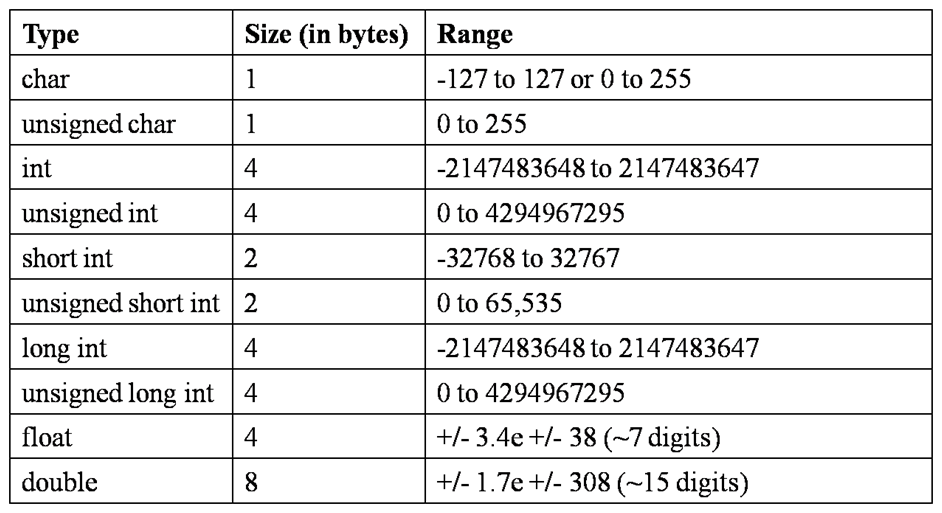
\includegraphics[width=1\textwidth, height=1\textheight, keepaspectratio]{./imgs/data_types_table.png}
	\caption{Tabelle dei tipi}
	\label{fig:data_types}
\end{figure}

\textsf{\small E dei wrappers sui tipi \textbf{unsigned} (ovvero senza segno, ovvero sempre e solo positivi), come: }\\

\begin{tabular}{cc}
	\color{myblue2}size\_t & corrisponde ad unsigned int \\
	\color{myblue2}uint8\_t & unsigned char \\
	\color{myblue2}uint16\_t & unsigned int  \\
	\color{myblue2}uint32\_t & unsigned long \\ 
\end{tabular} \\

\textsf{\small E altri tipi di dati per lavorare sui caratteri e sulle stringhe: }\\

\begin{tabular}{cc}
	\color{myblue2}string & (includere string) \\
	\color{myblue2}wchar\_t & wide char (per caratteri più grandi di 255) \\
\end{tabular}

\break

\textsf{\small Altri tipi di dati: } \\

\begin{tabular}{cc} %TODO: aggiungerne altri volendo.
	\color{myblue2}bool & Un booleano : o 0, ovvero FALSO/OFF o 1, ovvero TRUE/ON \\
	\color{myblue2}std::byte & 8 bit (definito in <cstddef> header file) \\
	\color{myblue2}register &  un registro\\ 
	\color{myblue2} auto &  trova la tipologia automaticamente\\
\end{tabular}\\

\textsf{\small Esistono anche altri tipi, ma quelli qui riportati sono tra i più comuni.}\\

\subsection{Cast}

\textsf{\small \textbf{Definizione: } Il \textbf{Cast} è un'operazione che permette di cambiare la tipologia di una variabile o di una determinata operazione matematica.} 

\textsf{\small Ovviamente, questa operazione potrebbe portare ad una perdita di dati, in particolare, quando facciamo un cast da una tipologia più grande (che occupa più spazio, più bits) ad una più piccola (che occupa meno spazio, meno bits) perché quella piccola non ha lo stesso spazio di immagazzinamento di quella grande.} 

\textsf{\small Per esempio se si fa un cast da una tipologia a 32 bit ad una a 8 bit, ovviamente si perderanno dei dati, perchè quella da 8 non può contenere gli stessi dati di una da 32.} \\

\textsf{\small Per fare un cast bisogna mettere, prima dell'operazione, tra parentesi la tipologia a cui si vuole castare. Esempio: (float) 5 / 2 = 3.5} \\

\begin{lstlisting}
	// Primo esempio:
	
	int a = 7, b = 2;
	float c;
	
	c = a / b; // Output : 3
	
	c = (float) a / b; // Output : 3.5
	
	// Secondo esempio:
	
	double d = 36.9;
	float f = 22.2;
	int x;
	
	x = (int) d; // Output : 36
	x = (int) f; // Output : 22
	
	// Ovviamente una variabile intera non può contenere i dati delle variabili con la virgola e quindi le informazioni sulla virgola vengono perse.
\end{lstlisting}

\textsf{\small Questo è un cast semplice, ci sono altre forme di cast un po' più complesse che vedremo in un altro capitolo.} \\

% -------------------------- SECTION: COSTANTI ---------------------------------------

\newpage

\section{Costanti}

\textsf{\small Una costante è un valore che non cambia mai.}\\

\textsf{\small Ci sono diversi tipi di costanti e con significato diverso, per esempio \color{myblue2} cost \normalcolor e \color{myblue2} constexpr. \normalcolor}\\

\subsection{const vs constexpr}

\begin{tabular}{|c|c|}
	\hline
	\textbf{const} & \textbf{constexpr} \\
	\hline
	\textsf{\small può essere composta da altre variabili a run-time} & \textsf{\small deve essere conosciuta a compile-time} \\
	%\hline
	\textsf{\small può essere usata solo per } & \textsf{\small può essere usata sia per member } \\
	\textsf{\small non-static member functions} & \textsf{\small e non-member functions} \\
	\textsf{\small } & \textsf{\small e anche costruttori} \\
	\hline
\end{tabular}\break

\subsection{static}

\subsubsection{Variabili statiche}

\textsf{\small Viene allocata per l'intera durata del programma. Anche se la funzione è chiamata molteplici volte, lo spazio allocato per la variabile statica è allocato una volta sola.} \\

\subsubsection{Membri statici delle classi} %TODO: sistemare questa parte.

\centering\textbf{Istanze delle classi come statiche} \\

\textsf{\small I distruttori (funzioni che rimuovo l'allocazione di memoria di un oggetto classe) vengono invocati soltanto dopo la fine del main (funzione principale da cui parte tutto il programma).} \break

\centering\textbf{Funzioni statiche in una classe} \\

\textsf{\small Queste possono soltanto accedere a dati statici o altre funzioni statiche.} \\

\subsection{static const}

\textsf{\small Per quanto riguarda \color{myblue2} static const \normalcolor possono ottenere un valore a compile time o a runtime, proprio come \color{myblue2} const, \normalcolor ma solo accessibili nella data funzione/classe.}\\

\subsection{static constexpr}

%TODO: scrivere qualcosa su static constexpr

\begin{figure}[ht]
	\centering
	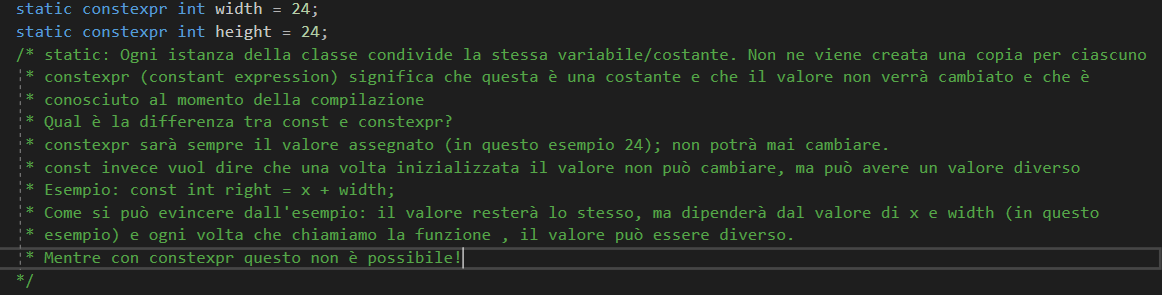
\includegraphics[width=1.2\textwidth, height=1.2\textheight, keepaspectratio]{./imgs/constexpr_e_const_differenze.png}
	\caption{Tipi di costanti}
	\label{fig:constants}
\end{figure}

% -------------------------- SECTION: ARRAYS E MATRICI -------------------------------

\section{Arrays e Matrici}

\subsection{Arrays}

\textsf{\small \textbf{Definizione: } Gli array sono dei contenitori di dati, una collezione di dati dello stesso tipo.} \\

\textsf{\small Il primo elemento di un array, come qualsiasi altra cosa in informatica è l'elemento 0, non l'elemento 1.}\\

\textsf{\small Quindi l'elemento di indice 0 è il primo elemento, quello di indice 1 è il secondo, quello di indice 2 è il terzo e cosi via..} \\

\begin{lstlisting}[language=C++]
	// tipologia nomeDelArray[ spazioOccupato ];
	
	double dArray[3];
	
	// Qui potremmo usare un loop per definire questi elementi, 
	// ma li vedremo dopo.
	dArray[0] = 12.4;
	dArray[1] = 37.9;
	dArray[2] = 19.1;
	
	// Possiamo assegnarli anche quando definiamo l'array.
	int array[5] = {7, 9, 12, 4, 11};
	
	// Potremmo anche non definire il size (spazio dell'array).
	int array2[] = {3, 6, 9};
	
	// Ma è raccomandabile usare dei contenitori come: std::vector 
	// oppure una lista.
	// Oppure dei puntatori.
	// Oppure dei smart pointers.
\end{lstlisting}

\subsection{Matrici}

\textsf{\small \textbf{Definizione: } Le matrici sono degli arrays organizzati su righe e colonne. Questo concetto è per una matrice di 2-dimensioni. La si può pensare proprio come una tabella, formata da righe e da colonne.} \\

\begin{lstlisting}
	#include <iostream> 
	
	// <iostream> è un file di intestazione (header file) della libreria standard per poter lavorare sull'input e sull'output.
	
	// tipologia nome\_matrice [righe][colonne];
	
	int matrix[3][3] = {{1,2,3}, {4,5,6}, {7,8,9}}
	
	for(int i = 0; i < 3; i++){
		for(int j = 0; j < 3; j++){
			std::cout << "elemento di riga " << i << " e colonna " << j << matrix[i][j] << std::endl;
		}
	}
\end{lstlisting}

\textsf{\small Ovviamente, come in matematica, è possibile eseguire varie operazioni sulle matrici, come: trasposizione, moltiplicazione, somma, sottrazione, ecc..(ma che qui non mostrerò).} \\ 

% -------------------------- SECTION: OPERATORI ARITMETICI ---------------------------

\section{Operatori Aritmetici}

\textsf{\small \textbf{Definizione: } Gli operatori aritmetici permettono di eseguire qualsiasi operazione aritmetica.} \\

\begin{itemize}
	\item \textsf{\small \textbf{+} : somma.}
	\item \textsf{\small \textbf{-} : sottrazione.}
	\item \textsf{\small \textbf{*} : moltiplicazione.}
	\item \textsf{\small \textbf{/} : divisione.}
	\item \textsf{\small \textbf{\%} : modulo, restituisce il resto della divisione.}
\end{itemize}

\begin{lstlisting}
	int a = 8, b = 3;
	
	a + b; // Output : 11
	
	a - b; // Output : 5
	
	a * b; // Output : 24
	
	a / b; // Output : 2
	
	a % b; // Output : 2 (resto della divisione)
	
\end{lstlisting}

% -------------------------- SECTION: OPERATORI RELAZIONALI --------------------------

\section{Operatori Relazionali}

\textsf{\small \textbf{Definizione: } Gli operatori relazionali servono per controllare la relazione tra due operandi. } \\

\begin{itemize}
	\item \textsf{\small \textbf{==} : per l'equivalenza; controllare se due operandi sono uguali.}
	\item \textsf{\small \textbf{!=} : per controllare se due operandi non sono equivalenti.}
	\item \textsf{\small \textbf{>} : per controllare se un operando è maggiore dell'altro}
	\item \textsf{\small \textbf{>=} : per controllare se un operando è maggiore o uguale all'altro.}
	\item \textsf{\small \textbf{<} : per controllare se un operando è minore di dell'altro.}
	\item \textsf{\small \textbf{<=} : per controllare se un operando è minore o uguale all'altro.}
\end{itemize}

\begin{lstlisting}
	int x = 5, y = 3;
	x == y // Output : FALSE
	x != y // Output : TRUE
	x > y // Output : TRUE
	x >= y // Output : TRUE
	x < y // Output : FALSE
	x <= y // Output : FALSE
	
\end{lstlisting}

% -------------------------- SECTION: OPERATORI BITWISE ------------------------------

\section{Operatori Bitwise}

\textsf{\small \textbf{Definizione: } Gli operatori bitwise servono per lavorare sui singolo bits di dati.} \\

\begin{itemize}
	\item \textsf{\small \textbf{\& (bitwise AND)} : permette di fare un AND bit a bit sui due operandi. Il risultato è 1 soltanto se entrambi sono 1.}
	\item \textsf{\small \textbf{| (bitwise OR)} : permette di fare un OR bit a bit su ogni bit dei due operandi. Il risultato è 1 se almeno uno dei due bits è a 1.}
	\item \textsf{\small \textbf{\^  (bitwise XOR)} : permette di fare uno XOR bit a bit su ogni bit dei due operandi. Il risultato è 1 se i due bits sono differenti.}
	\item \textsf{\small \textbf{$<<$ (left shift)} : prende due numeri. Shifta a sinistra i bits del primo operando, il secondo operando decide di quanti bits si deve shiftare il primo.}
	\item \textsf{\small \textbf{$>>$ (right shift)} : prende due numeri. Shifta a destra i bits del primo operando, il secondo operando decide di quanti bits si deve shiftare il primo.}
	\item \textsf{\small \textbf{\~ (bitwise NOT)} : prende un numero ed inverte tutti i bits.}
\end{itemize}

\begin{lstlisting}
	// a = 5 in binario è 00000101, b = 9 in binario è 00001001
	int a = 5, b = 9;
	
	a & b; // Output : 00000001
	
	a | b; // Output : 00001101
	
	a ^ b; // Output : 00001100
	
	~a; // Output : 11111010
	
	b << 1; // Output : 00010010
	
	b >> 1; // Output : 00000100
	
	
\end{lstlisting}

% ---------- SECTION: OPERATORI DI ASSEGNAMENTO E OPERATORI UNARI --------------------

\section{Operatori di Assegnamento e Operatori Unari}

\subsection{Operatori di Assegnamento}

\textsf{\small \textbf{Definizione: } Gli operatori di assegnamento sono usati per assegnare un valore alle variabili.} \\

\begin{itemize}
	\item \textsf{\small \textbf{=} : Operatore di assegnamento di un valore ad una variabile.}
	\item \textsf{\small \textbf{+=} : Combinazione di = e +, aggiunge l'operando di destra a quello di sinistra e lo assegna a quello di sinistra.}
	\item \textsf{\small \textbf{-=} : Combinazione di = e -, sottrae l'operando di destra a quello di sinistra e lo assegna a quello di sinistra.}
	\item \textsf{\small \textbf{*=} : Combinazione di = e *, moltiplica l'operando di destra a quello di sinistra e lo assegna a quello di sinistra.}
	\item \textsf{\small \textbf{/=} : Combinazione di = e /, divide l'operando di destra a quello di sinistra e lo assegna a quello di sinistra.}
	\item \textsf{\small \textbf{\%=} : Combinazione di = e \%, ottiene il resto dall'operando di destra a quello di sinistra e lo assegna a quello di sinistra.}
	\item \textsf{\small \textbf{$<<$=} : Combinazione di = e $<<$, left shifta l'operando di destra a quello di sinistra e lo assegna a quello di sinistra.}
	\item \textsf{\small \textbf{$>>$=} : Combinazione di = e $>>$, right shifta l'operando di destra a quello di sinistra e lo assegna a quello di sinistra.}
	\item \textsf{\small \textbf{\&=} : Combinazione di = e \&, bitwise AND sull'operando di destra a quello di sinistra e lo assegna a quello di sinistra.}
	\item \textsf{\small \textbf{\^ =} : Combinazione di = e \^, bitwise XOR sull'operando di destra a quello di sinistra e lo assegna a quello di sinistra.}
	\item \textsf{\small \textbf{|=} : Combinazione di = e |, bitwise OR sull'operando di destra a quello di sinistra e lo assegna a quello di sinistra.}
	\item \textsf{\small \textbf{$<>$=} : Bitwise shift left/right assignment} 
\end{itemize}

\begin{lstlisting}
	int x = 5; // = è un operatore di assegnamento.
	int y;
	
	y += 3; // += è un operatore di assegnamento ed è la combinazione dell'operatore = e l'operatore +. Scrivere y += 3; è identico a scrivere y = y + 3; (ovvero y è uguale a se stesso + 3).
	
	y -= 2; // identico a y = y - 2;
	
	y *= 4; // identico a y = y * 4; (* è un per, oppure viene usato nei puntatori)
	
	y /= 6; // identico a y = y / 6;
	
\end{lstlisting}

\subsection{Operatori Unari}

\textsf{\small \textbf{Definizione: } Gli operatori unari operano su un operando per produrre un nuovo valore.} \\

\begin{itemize}
	\item \textsf{\small \textbf{-} : nega il valore dell'operando.}
	\item \textsf{\small \textbf{++nome\_variabile} : Incremento di 1 prefix, prima incrementa l'operando prima che venga eseguito.}
	\item \textsf{\small \textbf{nome\_variabile++} : Incremento postfix, il valore verrà incrementato dopo che è stato usato.}
	\item \textsf{\small \textbf{- -nome\_variabile} : Decremento di 1 prefix, decrementa l'operando prima che venga usato. }
	\item \textsf{\small \textbf{nome\_variabile- -} : Decremento postfix, il valore verrà decrementato dopo che è stato usato.}
	\item \textsf{\small \textbf{\&nome\_variabile} : prima di una variabile, restituisce l'indirizzo di memoria della variabile in questione. In questo caso, NON è l'operatore bitwise AND \&.}
	\item \textsf{\small \textbf{!nome\_variabile} : operatore not, inverte lo stato logico dell'operando. Se è TRUE allora lo modifica in FALSE, se è FALSE allora diventa TRUE.}
\end{itemize}

\begin{lstlisting}
	int x = 3;
	
	-x; // l'operatore - nega il valore dell'operando.
	
	++x; // identico a scrivere x = x + 1; Questo è chiamato incremento prefisso, perché: in questo modo il valore dell'operando verrà alterato prima che venga usato.
	
	x++; // identico a scrivere x = x + 1; L'operatore ++ incrementa di 1 il valore della variabile in questione. Questo è chiamato incremento postfisso perché: in questo modo il valore verrà modificato dopo che è stato usato.
	
	--x; // identico a scrivere x = x - 1; Come per il ++ questo è un decremento prefisso.
	
	x--; // identico a scrivere x = x - 1; Decrementa di 1 il valore della variabile in questione. Decremento post fisso.
	
	&x; // l'operatore \&, prima di una variabile, restituisce l'indirizzo di memoria in cui la variabile risiede.
	
	bool y = true;
	
	!y; // Output : y è false;  l'operatore ! (not) inverte lo stato logico dell'operando.
	
\end{lstlisting}

% -------------------------- SECTION: OPERATORI LOGICI -------------------------------

\section{Operatori Logici}

\textsf{\small \textbf{Definizione: } Gli operatori logici servono per combinare due o più condizioni. Il risultato di un'operazione degli operatori logici è un booleano TRUE (VERO) o FALSE (FALSO).} \\

\begin{itemize}
	\item \textsf{\small \textbf{\&\& (logical AND)} : restituisce vero se tutte le condizioni sono vere.}
	\item \textsf{\small \textbf{|| (logical OR)} : restituisce vero se almeno una delle condizioni è vera.}
	\item \textsf{\small \textbf{! (logical NOT)} : restituisce vero se la condizione è falsa e restituisce falso se la condizione è vera.}
	\item \textsf{\small \textbf{!~} : Logical negation/bitwise complement} 
\end{itemize}

\begin{lstlisting}
	int x = 3, y = 6, z = 9;
	
	(x > y) || (y != z); // Output : TRUE, perché anche se x > y è FALSA, y != z è VERA.
	
	(y > x) && (y < z); // Output : TRUE perché entrambe sono vere.
	
	!(x > 7); // Output : TRUE, perché x non è maggiore di 7, quindi è falsa, ma il not inverte e quindi essendo la condizione falsa, il not la inverte in VERA.
	
\end{lstlisting}

% -------------------------- SECTION: ALTRI OPERATORI --------------------------------

\section{Altri Operatori}

\textsf{\small Ci sono altri operatori come: } \\

\begin{itemize}
	\item \textsf{\small \textbf{sizeof} : è usato per ottenere lo spazio che occupa una variabile.}
	\item \textsf{\small \textbf{,} : la virgola è usata sia come operatore che come separatore. valuta il primo operando e cancella il risultato, valuta il secondo operando e restituisce il suo valore.}
	\item \textsf{\small \textbf{Operatore Condizionale/Ternario} : condizione ? se vero esegui questo : se falso esegui questo.}
\end{itemize}

\begin{lstlisting}
	sizeof(char); // Output : 1
	sizeof(int); // Output : 4
	sizeof(float); // Output : 4
	sizeof(double); // Output : 8
	
	int a = 0;
	double d = 3.69;
	
	sizeof(a); // Output : 4
	sizeof(d); // Output : 4
	
	sizeof(a + d); // Output : 8
	
	int y = 2, x = 3; // Output : equivalente a int y = 2; int x = 3;
	
	x >= 0 ? "x è maggiore o uguale a 0" : "x è minore di 0"; // Output : "x è maggiore o uguale a 0".
\end{lstlisting}

% -------------------------- SECTION: IF STATEMENTS ----------------------------------

\newpage

\section{Condizione If}

\subsection{If|else if|else}

\textsf{\small \textbf{Definizione:} L'If statement permette di decidere se un certo blocco di codice verrà eseguito o no.} \\

\textsf{\small L'else statement permette di eseguire un altro blocco di codice, casomai la condizione sia falsa.} \\

\textsf{\small else if(condizione) statement permette di fare un'ulteriore controllo dopo al primo if statement. } \\

\subsection{Operatore Ternario}

\textsf{\small Un altro modo per valutare una condizione ed eseguire un codice è attraverso l'operatore ternario: condizione ? se è vera esegui questo : altrimenti esegui questo.} \\

\textsf{\small L'unica differenza con l'if è che si può eseguire una sola riga di codice sia nel caso la condizione sia vera sia falsa.} \\

\begin{lstlisting}
	if(condizione)
	{
		// Se (if) la condizione è vera esegui questo blocco di codide.
	} else {
		// Altrimenti (else) esegui questo blocco di codice.
	}

	// Esempio: Cerchiamo il valore maggiore.
	int x = 5, y = 3;
	
	if(x > y)
	{
		std::cout << "x è maggiore di y" << std::endl;
	} 
	else if(x == y){
		std::cout << "x ed y sono uguali" << std::endl;
	}
	else {
		std::cout << "x è minore di y" << std::endl;
	}

	// Qui invece cerchiamo il valore minore.
	int a = 8, b = 7;
	int min;
	
	min = a < b ? a : b;
	
	std::cout << "Il valore minimo è: " << min << std::endl;
\end{lstlisting}

\textsf{\small Se la riga da eseguire è 1 sola, allora si possono anche omettere le parentesi graffe.} \\

% -------------------------- SECTION: SWITCH -----------------------------------------

\section{Switch}

\subsection{Switch|Cases|Break}

\textsf{\small \textbf{Definizione: } Gli switch statements valutano una data espressione ed in base al valore di quella espressione, eseguono un determinato blocco di codice.} \\

\textsf{\small Le possibili espressioni che si possono mettere nello switch sono: }

\begin{itemize}
	\item \textsf{\small Un numero intero, \color{myblue2}int}
	\item \textsf{\small Un enumeratore, \color{myblue2}enum}
	\item \textsf{\small Un carattere, \color{myblue2}char \normalcolor che è un piccolo intero tra -128 e + 127.}
\end{itemize}

\textsf{\small Le varie scelte sono indicate nel \textbf{case}.} \\

\textsf{\small I cases son tutti collegati fra loro e quindi per far si che solo un blocco di codice venga eseguito utilizziamo la keyword \textbf{break} per poter uscire dallo switch una volta che il codice è stato eseguito.} 

\textsf{\small Se non mettessimo il \textbf{break} allora una volta eseguito un case, il codice che è sequenziale, eseguirebbe il case sotto. Possiamo evitare di metterlo se vogliamo che alcuni case eseguino lo stesso codice.} \\

\subsection{Default Case}

\textsf{\small Infine c'è un case \textbf{default} nel caso che il valore valutato non sia presente tra i case. Questo case è opzionale, quindi si può anche non includere.}

\textsf{\small Per il \textbf{default} non serve il \textbf{break} perchè è comunque l'ultimo case, però volendo lo si può sempre mettere.} \\

\begin{lstlisting}
	int scelta = 3;
	
	switch(scelta){
		case 1:
			std::cout << "Scelta: 1" << std::endl;
			// Blocco di codice per il case 1.
			break;
		case 2:
			std::cout << "Scelta: 2" << std::endl;
			// Blocco di codice per il case 2.
			break;
		case 3:
			std::cout << "Scelta: 3" << std::endl;
			// Blocco di codice per il case 3.
			break;
		default:
			std::cout << "Nessuna scelta o scelta non prevista." << std::endl;
			// Blocco di codice per il default case.
			break;
	}
\end{lstlisting}

% -------------------------- SECTION: LOOPS ------------------------------------------

\newpage

\section{Loops}

\textsf{\small \textbf{Definizione: } I loops (cicli) ci permettono di ripetere un dato blocco di codice per un determinato o indeterminato numero di volte.} \\

\subsection{While}

\textsf{\small I while loops ci permettono di eseguire un ciclo quando non conosciamo esattamente il numero di iterazioni. } \\

\textsf{\small La condizione del while viene valutata, se possibile entra dentro al loop altrimenti lo salta ed esegue il codice dopo.}

\textsf{\small Ad ogni iterazione la condizione viene controllata, se vera il ciclo continua, se falsa il ciclo viene interrotto.} \\

\begin{lstlisting}
	while(condizione){
		// Blocco di codice da eseguire.
	}

	int x = 3;
	
	while(x < 5){
		std::cout << "Ciao per la " << x << "a volta" << std::endl;
		x++; // indentico a x = x + 1
	}
\end{lstlisting}

\subsection{Do-While}

\textsf{\small Nel Do while rispetto al singolo while, si entra almeno una volta all'interno del ciclo, poi come nel while viene controllata la condizione e se vera il ciclo continua altrimenti verrà interrotto.} \\

\begin{lstlisting}
	do{
		// Blocco di codice da eseguire.
	}while(condizione); // da notare il ; dopo il while.

	int x = 2;
	
	do{
		std::cout << "Hello World!" << std::endl;
		x++;
	}while(x < 1);
\end{lstlisting}

\subsection{Continue}

\textsf{\small La keyword \textbf{continue} è simile alla keyword \textbf{break}, ma invece di terminare l'esecuzione (del loop, dello switch, ecc..) , passa alla prossima iterazione del loop.}\\

\begin{lstlisting}
	int a = 5;
	do {
		if(a == 10){
			a++;
			continue;
		}
		std::cout << "Valore di a: " << a << std::endl;
		a++;
	} while( a < 20);
\end{lstlisting}

\subsection{goto}

\textsf{\small La keyword \textbf{goto} permette di fare un salto incondizionato verso una label (etichetta).}

\textsf{\small Potrebbe essere utile per uscire dai cicli annidati (nested loops).}

\textsf{\small L'uso del \textbf{goto} è scoraggiato ed è considerato una \emph{bad practice} perché porta a quello che è definito \emph{spaghetti code}, ovvero ad un codice destrutturato e difficile da mantenere.} \\

\begin{lstlisting}
	int a = 10;
	
	LOOP:do {
		if( a == 15) {
			// skip the iteration.
			a = a + 1;
			goto LOOP;
		}
		cout << "value of a: " << a << endl;
		a = a + 1;
	} 
	while( a < 20 );
\end{lstlisting}

\subsection{For}

\textsf{\small Il for loop è composto da tre parti: l'inizializzazione della variabile contatore, la condizione, ed aggiornamento della variabile contatore. }

\textsf{\small A differenza del while loop, in questo conosciamo già a priori quanti cicli faremo.}

\textsf{\small Ad ogni iterazione del ciclo, la variabile contatore viene aggiornata.} \\

\begin{lstlisting}
	for(inizializzazione; condizione; aggiornamento variabile){
		// Codice da eseguire.
	}

	int n = 4;
	
	for(int i = 0; i < n; i++){
		// Codice da eseguire
	}
\end{lstlisting}

\subsection{Foreach}

%TODO: aggiungere la ref ai for each

\textsf{\small Questo loop è un po' più complicato e si avvale degli iteratori che verrano spiegati più avanti in un altro capitolo.} %\ref{}}

\textsf{\small È definito nel file di intestazione \textbf{\#include <algorithm>}.} \\

\subsection{Cicli annidati}

\textsf{\small Si può inserire un loop dentro ad un altro loop (cicli annidati o nested loops).} \\

\subsection{Cicli Infiniti}

\textsf{\small Bisogna fare attenzione a non creare cicli infiniti, che come dice la parola vanno ad oltranza, rallentano e bloccano il programma.}\\

\begin{lstlisting}
	for( ; ; ){
		std::cout << "Loop Infinito" << std::endl;
	}
\end{lstlisting}

% -------------------------- SECTION: ENUMS ------------------------------------------

\section{Enumeratori}

\textsf{\small \textbf{Definizione: } Gli enumeratori sono dei tipi di dati definiti dagli utenti ed usati per assegnare nomi a delle costati intere, il che rende il codice semplice da leggere.}

\textsf{\small Il primo elemento di un enum è di indice 0, ammeno che non lo si cambi, se lo si cambia, di conseguenza, cambiano anche tutti gli altri sotto.} \\

\begin{lstlisting}
	enum Days {Lunedi, Martedi, Mercoledi, Giovedi, Venerdi, Sabato, Domenica};
	Days day = Venerdi;
	
	if(day == Venerdi){
		std::cout << "Oggi è venerdi!" << std::endl;
	}
	
	enum Year {
		GENNAIO = 1,
		FEBBRAIO,
		MARZO,
		APRILE,
		MAGGIO,
		GIUGNO,
		LUGLIO,
		AGOSTO,
		SETTEMBRE,
		OTTOBRE,
		NOVEMBRE,
		DICEMBRE
	};

	Year mese = FEBBRAIO;
	std::cout << "Siamo nel " << mese << "o mese dell'anno" << std::endl;

	enum Colors {
		ROSSO,
		BLU,
		VERDE,
		GIALLO,
		ARANCIONE,
		GRIGIO,
		VIOLA,
		ROSA,
		NERO,
		BIANCO
	};	

	Colors colore = Colors.ARANCIONE;
	std::cout << "Colore di indice: " << colore << std::endl;
	
	// Per poter vedere il nome dell'enum e non il suo valore, bisogna utilizzare una mappa o uno switch o altro.
\end{lstlisting}

% -------------------------- SECTION: VECTORS ----------------------------------------

%\section{Vectors}

% I vectors potrei anche metterli nel secondo capitolo.

%TODO: definizione dei vettori
%TODO: a cosa servono.

% -------------------------- SECTION: PUNTATORI --------------------------------------

\newpage

\section{Puntatori}

\textsf{\small \textbf{Definizione: } Un puntatore è una variabile che contiene l'indirizzo di memoria di un' altra variabile. Si può dire che questa variabile punta ad un' altra.} \\

\textsf{\small Per creare un puntatore usiamo l'operatore \textbf{*} che è lo stesso usato anche per la moltiplicazione.}

\textsf{\small Usiamo l'operatore \textbf{\&} (indirizzo) per ottenere l'indirizzo di una variabile.} 

\textsf{\small Per ottenere il valore della variabile a cui il puntatore punta usiamo l'operatore \textbf{*} (dereferenza).}\\

\begin{lstlisting}
	int x = 5;
	int* ptr; // puntatore ad intero
	
	ptr = &x; // il puntatore ptr punta alla variabile x
	
	std::cout << var << std::endl; // Output : 5
	std::cout << ptr << std::endl; // Output : indirizzo di x
	std::cout << *ptr << std::endl; // Output : 5
\end{lstlisting}

\subsection{Aritmetica dei puntatori}

\textsf{\small Sui puntatori è possibile eseguire delle operazioni aritmetiche:} \\

\begin{itemize}
	\item \textsf{\small Icremento|Decremento di un puntatore.}
	\item \textsf{\small Addizione di un intero ad un puntatore.}
	\item \textsf{\small Sottrazione di un intero ad un puntatore.}
	\item \textsf{\small Sottrazione di due puntatori dello stesso tipo.}
\end{itemize}

\begin{lstlisting}
	// Primo esempio
	#define MAX 3
	int var[MAX] = {3, 6, 9};
	int *ptr1, *ptr2;
	
	ptr1 = &var[MAX - 1];
	
	while ( ptr <= &var[MAX - 1] ) {
		std::cout << "Address of var[" << i << "] = ";
		std::cout << ptr << endl;
		
		std::cout << "Value of var[" << i << "] = ";
		std::cout << *ptr << endl;
		
		// point to the previous location
		ptr++;
		i++;
	}
	
	// Secondo esempio
	
	int x[10];
	int *p1, *p2;
	int i;
	
	p1 = &x[3]; // P1 punta a x[3]
	p2 = p1 + 2; // P2 punta a x[5]
	
	p1 += 6; // P1 punta ad x[9];
	
	p2 = p1 - 3; // P2 punta ad x[6];
	p1 -= 7; // P1 punta ad x[2];
	
	i = p2 - p1; // i : 6 - 2 = 4
	i = p1 - p2; // i : 2 - 6 = -4
\end{lstlisting}

\subsection{Puntatori a puntatori}

\textsf{\small Come esistono i puntatori ad una variabile, esistono anche dei puntatori ad altri puntatori.} \\

\textsf{\small Creiamo un puntatore ad un puntatore semplicemente aggiungendo un ulteriore * al singolo puntatore.}

\begin{lstlisting}
	int var = 369;
	int *ptr;
	int **pptr;
	
	ptr = &var;
	
	pptr = &ptr;
	
	std::cout << "Valore di var: " << var << std::endl; // Output: Valore di var: 369
	std::cout << "Valore di *ptr: " << var << std::endl; // Output: Valore di *ptr: 369
	std::cout << "Valore di **pptr: " << var << std::endl; // Output: Valore di **pptr: 369
\end{lstlisting}

%TODO: volendo puntatori ad array.
%TODO: volendo puntatori a matrici.

% -------------------------- SECTION: REFERENCE --------------------------------------

\section{References}

\textsf{\small \textbf{Definizione: } Una reference è come un alias, ovvero un altro nome per una variabile che già esiste. Come i puntatori è implementata attraverso la memorizzazione dell'indirizzo di memoria della suddetta variabile.} \\

\textsf{\small Definiamo una reference attraverso l'operatore \textbf{\&} prima del nome della variabile.}

\textsf{\small Se facciamo qualcosa alla reference, all'alias, di conseguenza lo facciamo anche alla variabile a cui si riferisce.} \\

\begin{lstlisting}
	int x = 10;
	
	int& ref = x; // Questa è una reference alla variabile x.
	
	ref = 20;
	std::cout << "x: " << x << std::endl; // Output : 20
	
	x = 30;
	std::cout << "ref: " << ref << std::endl; // Output : 30
\end{lstlisting}

\begin{figure}[ht]
	\centering
	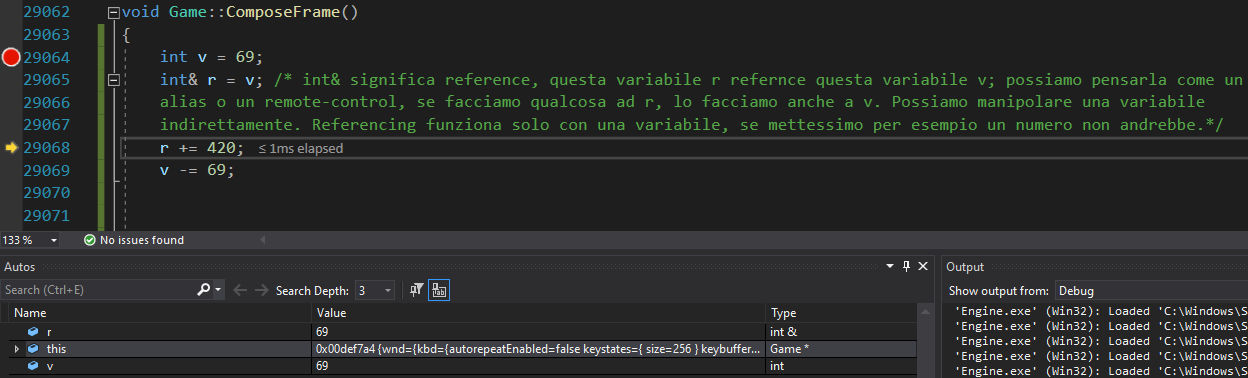
\includegraphics[width=1.2\textwidth, height=1.2\textheight, keepaspectratio]{./imgs/References.png}
	\caption{Reference}
	\label{fig:references1}
\end{figure}

\begin{figure}[ht]
	\centering
	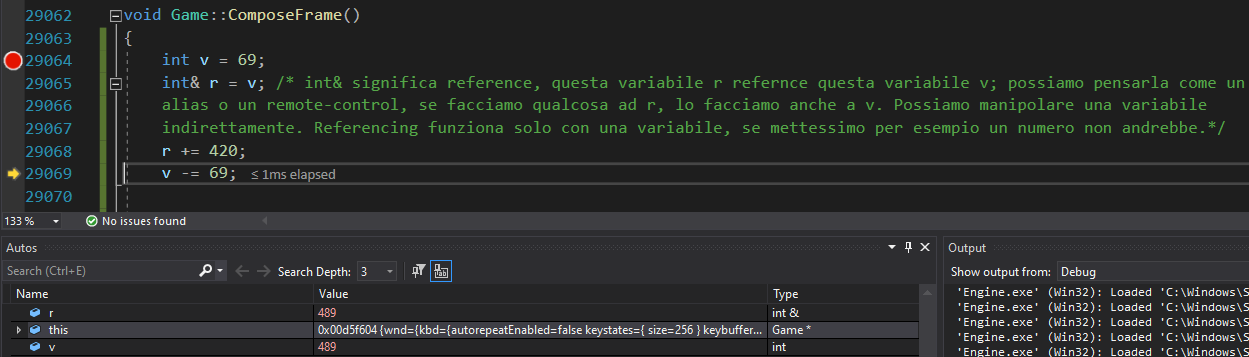
\includegraphics[width=1.2\textwidth, height=1.2\textheight, keepaspectratio]{./imgs/References2.png}
	\caption{Reference}
	\label{fig:references2}
\end{figure}

\subsection{References vs Puntatori}

\begin{tabular}{|c|c|}
	\hline
	\textbf{Reference} & \textbf{Pointers} \\
	\hline
	\textsf{\small Riferiscono ad una variabile } & \textsf{\small Memorizzano un indirizzo } \\
	\textsf{\small con un altro nome} & \textsf{\small di una variabile} \\
	\hline
	\textsf{\small Non possono avere un valore \color{myblue2}NULL \normalcolor.} & \textsf{\small Possono avere un valore \color{myblue2}NULL \normalcolor.} \\
	\hline
	\textsf{\small Deve essere inizializzata } & \textsf{\small Può anche non essere inizializzata } \\
	\textsf{\small alla dichiarazione} & \textsf{\small alla dichiarazione} \\
	\hline
	\textsf{\small Condivide la stessa memoria  } & \textsf{\small Ha un proprio spazio e } \\
	\textsf{\small con la variabile originale, } & \textsf{\small indirizzo di memoria } \\
	\textsf{\small ma prende anche dello spazio nello stack.} & \textsf{\small sullo stack.} \\
	\hline
	\textsf{\small Non può essere riassegnato.} & \textsf{\small Può essere riassegnato.} \\
	\hline
	\textsf{\small Hanno un solo livello di indirezione.} & \textsf{\small Si possono avere puntatori } \\
	\textsf{\small } & \textsf{\small a puntatori per livelli extra } \\
	\textsf{\small } & \textsf{\small di indirezione.} \\
	\hline
	\textsf{\small Non c'è la aritmetica delle references} & \textsf{\small C'è l'aritmetica dei puntatori.} \\
	\hline
	%\textsf{\small } & \textsf{\small } \\
	%\hline
\end{tabular}

\subsection{NULL vs nullptr}

\textsf{\small \textbf{NULL} portato dal C corrisponde semplicemente a 0 (è una macro) e non necessariamente ad un puntatore. Mentre \textbf{nullptr} (è un \emph{pointer literal}), specifico del C++ è sempre un puntatore, di tipo \emph{std::nullptr\_t} (è un prvalue di tipo nullptr\_t), un puntatore a tutti gli effetti. Se lo si cerca di adottare ad un'altra variabile, tipo ad un int darà errore.} \\

\textsf{\small \textbf{nullptr} è implicitamente convertibile a qualsiasi tipo di puntatore.} \\

\begin{lstlisting}
	#include <iostream>
	
	int main()
	{
		int ptr = nullptr; // Errore.
		
		int *ptr = nullptr; // Va bene.
		return 0;
	}
\end{lstlisting}

\begin{lstlisting}
	#include <iostream>
	
	void func(int n);
	void func(char *s);
	
	func ( NULL ); // Quale delle due funzioni verrà chiamata? La prima, perché NULL è 0 e quindi un int.
\end{lstlisting}

\textsf{\small \textbf{nullptr} è definito nell'header \textbf{<cstddef>}, ma non serve includerlo perché è una \emph{built-in} keyword.} \\ 

% -------------------------- SECTION: STRINGHE ---------------------------------------

\newpage

\section{Stringhe}

%TODO: mettere std::string qui? E anche char? e c-strings? anche la Tabella ASCII?
%Prima questa parte dei char, C-string, std::string stava nella sezione Tipi di Dati

\subsection{Char}

\textsf{\small \textbf{Definizione: } Un \textbf{char} è usato per memorizzare un singolo carattere} \\

\textsf{\small Alternativamente, si possono usare i valori ASCII per indentificare le lettere} \\

\begin{lstlisting}
	char linguaggio = 'C';
	
	char linguaggio = 67; // 67 corrisponde a C nella tabella ASCII.
\end{lstlisting}

\subsection{C-string}

\textsf{\small Per creare una stringa in C facciamo un array (contenitore di dati dello stesso tipo) di char.}

\textsf{\small Il \textbf{'\textbackslash0'} è il \textbf{NUL terminator} che denota la fine di una C-stringa. } \\

\begin{lstlisting}
	char s[] = "prova";
	
	// Oppure possiamo scriverlo:
	char s[] = { 'p', 'r', 'o', 'v', 'a', '\0'};
	
	// '\textbackslash0' è il NUL terminator, denota la fine di una stringa.
\end{lstlisting}

\subsection{char*}

\textsf{\small Un puntatore a char memorizza la locazione iniziale di una C-string (una stringa in C). } \\

\begin{lstlisting}
	char s = "prova";
	
	// Possiamo far puntatore al puntatore la prima cella dell'array così..
	char* p = &(s[0]);
	
	// ..oppure in maniera più coincisa così:
	char *p = s;
\end{lstlisting}

\subsection{Tabella ASCII}

\textsf{\small \textbf{Definizione: } La tabella \textbf{ASCII} (\emph{American Standard Code for Information Interchange}) è un codice per la codifica di caratteri.} \\

\textsf{\small Inizialmente era basata su codici di 7 bit, quindi per un totale di $2^7 = 128$ caratteri. Venne poi estesa ad 8 bit, per un totale di $2^8 = 256$ caratteri.} \\

\begin{figure}[ht]
	\centering
	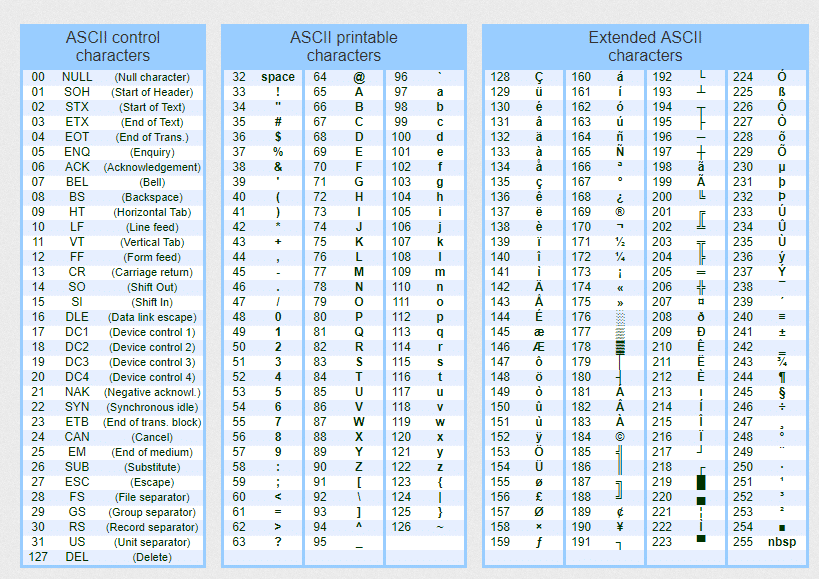
\includegraphics[width=1.2\textwidth, height=1.2\textheight, keepaspectratio]{./imgs/ascii_table2.png}
	\caption{Tabella ASCII}
	\label{fig:ascii_table}
\end{figure}

\subsection{std::string}

\textsf{\small \textbf{Definizione: } Il C++ ha una propria definizione per rappresentare una sequenza di caratteri come un oggetto di una classe. Questa classe è chiamata std::string. Questa memorizza i caratteri come una sequenza di bytes con la funzionalità di poter accedere al singolo carattere byte.} \\

\textsf{\small La classe std::string ha diverse funzioni, come: } 

\begin{tabular}{|c|c|}
	\hline
	\textbf{Funzione} & \textbf{Definizione} \\
	\hline
	\textbf{length()} & \textsf{\small restituisce la lunghezza della stringa.} \\
	\hline
	\textbf{capacity()} & \textsf{\small restituisce la capacità allocata alla stringa che } \\
	\textbf{} & \textsf{\small può essere più o meno la lunghezza.} \\
	\hline
	\textbf{resize()} & \textsf{\small cambia la grandezza della stringa che può essere aumentata o diminuita.} \\
	\hline
	\textbf{shrink\_to\_fit()} & \textsf{\small diminuisce la grandezza della stringa e la rende uguale } \\
	\textbf{} & \textsf{\small al minimo della capacità della stringa.} \\
	\textbf{} & \textsf{\small Utile per salvare ulteriore memoria se siamo sicuri } \\
	\textbf{} & \textsf{\small di non dover aggiungere altri caratteri.} \\
	\hline
	%\textbf{} & \textsf{\small } \\
\end{tabular} 

\textsf{\small Queste sono solo alcune delle funzioni della classe string.} \\

\begin{lstlisting}
	std::string str = "Ciao a tutti";
	
	str.resize(4); 
	
	std::cout << "Stringa dopo resize: " << str << std::endl; // Output : Stringa dopo resize: Ciao
	
	std::cout << "Capacità della stringa: " << str.capacity() << std::endl; // Output : Capacità della stringa: 12
	
	std::cout << "Lunghezza della stringa: " << str.length() << std::endl; // Output : Lunghezza della stringa: 4
	
\end{lstlisting}

\subsection{char* vs std::string vs char[]}

\subsubsection{Usare char*}

\begin{lstlisting}
	char *str = "prova";
\end{lstlisting}

\begin{tabular}{|c|c|}
	\hline
	\color{red} CONS & \color{Green} PROS \\
	\hline
	\textsf{\small In C va bene, ma in C++ è deprecato,  } & \textsf{\small Basta un singolo puntatore per  } \\
	\textsf{\small perché in C le stringhe sono array di char,} & \textsf{\small l'intera stringa. È efficiente } \\
	\textsf{\small mentre in C++ sono array di char costanti.} & \textsf{\small a livello di memoria.} \\
	\hline
	\textsf{\small Non possiamo modificare la stringa dopo, } & \textsf{\small Non c'è bisogno  } \\
	\textsf{\small possiamo semplicemente far puntare ad un'altra stringa.} & \textsf{\small di dichiarare la lunghezza } \\
	\textsf{\small } & \textsf{\small della stringa all' inizializzazione.} \\
	\hline
\end{tabular}

\subsubsection{Usare std::string}

\begin{lstlisting}
	std::string s = "prova";
\end{lstlisting}

\begin{tabular}{|c|c|}
	\hline
	\color{red} CONS & \color{Green} PROS \\
	\hline
	\textsf{\small } & \textsf{\small Con C++ std::string è la migliore via,  } \\
	\textsf{\small } & \textsf{\small perché ha delle funzioni di ricerca,} \\
	\textsf{\small } & \textsf{\small rimpiazzo e manipolazione migliori.} \\
	%\textsf{\small } & \textsf{\small } \\
	\hline
\end{tabular}

\subsubsection{Casi in cui preferire char* ad std::string}

\begin{itemize}
	\item \textsf{\small Quando si ha a che fare con livelli bassi di accesso, come interagire con il sitema operativo. Anche se std::string::c\_str dovrebbe occuparsi di quello.}
	\item \textsf{\small Compatibilità con del vecchio codice in C (Anche se la funzione std::string::c\_str dovrebbe già in largo modo occuparsi di questo).}
	\item \textsf{\small Per risparmiare memoria (std::string sicuramente occupa di più).}
\end{itemize}

\subsubsection{Usare char[]}

\begin{lstlisting}
	// In realtà ci bastano 5 spazi nell'array, però se poi dopo vogliamo fare
	// concatenazioni o manipolazioni sulle altre stringhe, ci servirà altro spazio.
	char stringa[128] = "prova";
\end{lstlisting}

\begin{tabular}{|c|c|}
	\hline
	\color{red} CONS & \color{Green} PROS \\
	\hline
	\textsf{\small È un array allocato staticamente che } & \textsf{\small Possiamo modificare la stringa } \\
	\textsf{\small consuma spazio nello stack.} & \textsf{\small anche in un altro stage del programma.} \\
	\hline
	\textsf{\small Dobbiamo utilizzare array di grandi dimensioni  } & \textsf{\small } \\
	\textsf{\small per poter concatenare o manipolare le altre stringhe,} & \textsf{\small } \\
	\textsf{\small visto che lo spazio dell'array è fissato dall'inizio.} & \textsf{\small } \\
	\hline
\end{tabular}

\subsection{Escape characters}

\textsf{\small \textbf{Definizione: } Le sequenze di fuga sono usate per rappresentare certi caratteri speciali nelle stringhe e nei caratteri. } \\

\textbf{Caratteri di controllo: } \\

\textsf{\small Compatibili con l'encoding ASCII.} \\

%TODO: magari da tradurre in italiano il resto e o lasciare qui o all'inizio dopo il cast.

\begin{tabular}{|c|c|}
	\hline
	\textbf{Escape sequence} & \textbf{Definizione} \\
	\hline
	\textsf{\small \textbf{$\backslash$a} : \textbf{$\backslash$x07}} & \textsf{\small alert (bell)} \\
	\hline
	\textsf{\small \textbf{$\backslash$b} : \textbf{$\backslash$x08}} & \textsf{\small backspace} \\
	\hline
	\textsf{\small \textbf{$\backslash$t} : \textbf{$\backslash$x09}} & \textsf{\small horizontal tab} \\
	\hline
	\textsf{\small \textbf{$\backslash$n} : \textbf{$\backslash$x0A}} & \textsf{\small newline (or line feed)} \\
	\hline
	\textsf{\small \textbf{$\backslash$v} : \textbf{$\backslash$x0B}} & \textsf{\small vertical tab} \\
	\hline
	\textsf{\small \textbf{$\backslash$f} : \textbf{$\backslash$x0C}} & \textsf{\small form feed} \\
	\hline
	\textsf{\small \textbf{$\backslash$r} : \textbf{$\backslash$x0D}} & \textsf{\small carriage return} \\
	\hline
	\textsf{\small \textbf{$\backslash$e} : \textbf{$\backslash$x1B}} & \textsf{\small escape (non-standard GCC extension)} \\
	\hline
\end{tabular} \break

\textbf{Caratteri di punteggiatura: } \\

\begin{tabular}{|c|c|}
	\hline
	\textbf{Escape sequence} & \textbf{Definizione} \\
	\hline
	\textsf{\small \textbf{$\backslash$"}} & \textsf{\small quotation mark} \\
	\hline
	\textsf{\small \textbf{$\backslash$'}} & \textsf{\small apostrophe} \\
	\hline
	\textsf{\small \textbf{$\backslash$?}} & \textsf{\small question mark (used to avoid trigraphs)} \\
	\hline
	\textsf{\small \textbf{$\backslash\backslash$}} & \textsf{\small backslash} \\
	\hline
\end{tabular} \break

\textbf{Caratteri di referenze numeriche: } \\

\begin{tabular}{|c|c|}
	\hline
	\textbf{Escape sequence} & \textbf{Definizione} \\
	\hline
	\textsf{\small \textbf{$\backslash$}} & \textsf{\small + 3 cifre in ottale} \\
	\hline
	\textsf{\small \textbf{$\backslash$x}} & \textsf{\small + qualsiasi cifra in esadecimale} \\
	\hline
	\textsf{\small \textbf{$\backslash$u}} & \textsf{\small + 4 cifre esadecimali} \\
	\hline
	\textsf{\small \textbf{$\backslash$U}} & \textsf{\small + 8 cifre esadecimali} \\
	\hline
	\textsf{\small \textbf{$\backslash$0} = \textbf{$\backslash$00} = $\backslash$000} & \textsf{\small octal escape for null character} \\
	\hline
\end{tabular}

% -------------------------- SECTION: FUNZIONI ---------------------------------------

\newpage

\section{Funzioni}

\textsf{\small \textbf{Definizione: } Una funzione è un blocco di codice che esegue una specifico compito e può essere richiamato quando si vuole.} \\

\textsf{\small Le funzioni sono composte da: un tipo di dato di ritorno che è ciò che la funzione restituisce dopo esser stata eseguita, un nome, degli eventuali parametri ed racchiusa tra due parentesi graffe il corpo, il blocco di codice.}

\textsf{\small Per eseguire la funzione basta richiamarla col suo nome e passare gli eventuali parametri.} \\

\subsection{return}

\textsf{\small La keyword \textbf{return} permette di restituire un valore/oggetto dalla funzione.} \\

\begin{lstlisting}
	// tipologia nome\_funzione(parametri)
	{
		// Blocco di codice della funzione.
	}
	
	// Questa funzione restituisce un intero, si chiama somma, prende due parametri interi a e b e restituisce la somma tra a e b. 
	int somma(int a, int b){
		return a + b;
	}
	
	// Fuori dalla funzione
	int x = 3, y = 5;
	// chiamiamo la funzione somma, gli passiamo i parametri e il valore di ritorno lo assegniamo alla variabile intera z.
	int z = somma(x, y); // Output z : 8
\end{lstlisting}

\textsf{\small Tutto ciò che è creato all'interno della funzione è locale alla funzione e quindi non accessibile da fuori.} \\

\textsf{\small I nomi dei parametri sono soltanto dei placeholders. Potremmo anche non metterli e lasciare solo le tipologie, ma poi per poterli referenziare nella funzione non sapremmo come fare.}

\textsf{\small I parametri che vengono passati alla funzione sono anch'essi locali, a meno che non li si passano attraverso dei puntatori.} \\

\textsf{\small I parametri passati, a meno che con puntatori, sono delle copie delle variabili passate come parametro, e qualsiasi modifiche di queste copie non ha un effetto sui parametri passati.} \\

\begin{lstlisting}
	// Questa è una funzione che restituisce un boolean (0 o 1 (VERO o FALSO)), chiamata isGreater che prende due variabili intere a e b come parametri e restituisce se true se la variabile a è maggiore della variabile b, altrimenti false.
	
	// Questa funzione si potrebbe scrivere così..
	bool isGreater(int a, int b)
	{
		if(a > b){
			return a;
		} else {
			return b;
		}
	}

	//.. Oppure si potrebbe anche scrivere così.
	bool isGreater(int a, int b)
	{
		return a > b;
	}

	// Detto questo, per questo tipo di operazioni, ci sono già delle funzioni della libreria Standard ben più ottimizzate. Per questo esempio si potrebbe usare std::max.
\end{lstlisting}

\subsection{void}

\textsf{\small Se non volessimo ritornare niente dovremmo usare la tipologia \textbf{void}, questo tipo di funzione (che non ritorna niente) è chiamata \textbf{procedura}.} \\

\subsection{main}

\textsf{\small Il \textbf{main} è la funzione principale di qualsiasi programma in C/C++, da esso parte il tutto, ha origine tutto.} \\

\begin{lstlisting}
	int main(){
		return 0;
	}
\end{lstlisting}

\subsection{Funzioni ricorsive}

\textsf{\small Le funzioni ricorsive sono delle funzioni che richiamano se stesse per raggiungere un risultato.} \\

%TODO: fixare funzioni
\begin{lstlisting}
	// Il fattoriale di un numero, o anche scritto n! è n * (n - 1)
	// 4! = 4 * 3 * 2 * 1 = 24
	int fattoriale(int n)
	{
		if((n == 0) || (n == 1))
			return 1;
		else
			return n * fattoriale(n - 1);
	}

	// Questa funzione si potrebbe anche scrivere
	int fattoriale(int n)
	{
		// Le parentesi nella condizione non servirebbero, le lascio per chiarezza
		return ((n == 0) || (n == 1)) ? 1 : n * fattoriale(n - 1);
	}

	// Fibonacci è una serie in cui i due primi elementi sono 1 e dove ogni elemento è uguale alla somma dei due termini precedenti. 
	
	int fibonacci(int x)
	{
		// Le parentesi nella condizione non servirebbero, le lascio per chiarezza
		return ((x == 1) || (x == 0)) ? x : fibonacci(x - 1) + fibonacci(x - 2);
	}

	int main()
	{
		int x = 4;
		std::cout << "Fattoriale di " << x << " e\': " << fattoriale(x) << std::endl; // Output : Fattoriale di 4 è 24.
		
		int y = 15;
		std::cout << "Fibonacci di " << y << " e\' " << fibonacci(15) << std::endl; // Output : Fibonacci di 15 è 610.
		return 0;
	}
\end{lstlisting}

%TODO: funzioni e i vari casi dei const e dove viene posizionato.

%TODO: funzioni pass by value, by reference, ecc..

\subsection{Argomenti passati per valore}

\textsf{\small Quindi, quando passiamo dei valori (e non degli indirizzi di memoria alle variabili), si dice che passiamo gli argomenti \textbf{per valore}, quindi una copia delle variabili passate viene creata ed usata nelle funzioni. }

\textsf{\small Quindi noi non operiamo direttamente sulle variabili passate, ma sulle loro copie. Questo non ci permette di poter modificare le variabili passate.} \\

\begin{lstlisting}
	int sottrazione(int a, int b)
	{
		return a - b;
	}

	// Fuori dalla funzione
	int x = 5, y = 3;
	int z = sottrazione(x, y); // Output: 2
\end{lstlisting}

\subsection{Argomenti passati per referenza}

\textsf{\small Per poter effettivamente modificare le variabili che abbiamo passato per argomento, dobbiamo passarle con i puntatori, dobbiamo passare i loro indirizzi di memoria. Questo si chiama passare argomenti \textbf{per referenza}.} \\

\textsf{\small Se, per esempio, volessimo sostituire i valori di due variabili e li passassimo per valore, non riusciremmo.} \\

\begin{lstlisting}
	// Parte 1: Usare argomenti passati per valore.
	void swap(int a, int b)
	{
		int temp = a;
		a = b;
		b = temp;
	}

	// Fuori dalla funzione
	int x = 5, y = 3;
	swap(x, y); 
	std::cout << "Valore di x dopo lo swap: " << x << std::endl; // Output : 5
	std::cout << "Valore di y dopo lo swap: " << y << std::endl; // Output : 3
	// Non funziona, noi vorremmo cambiare i valori di x ed y, ma così non funziona, perchè stiamo lavorando sulle copie delle variabili, non sulle variabili stesse.
	
	// Parte 2: Usare argomneti passati per referenza
	void swap(int *a, int *b)
	{
		int temp = *a;
		*a = *b;
		*b = temp;
	}

	// Fuori dalla funzione
	int x = 5, y = 3;
	swap(x, y);
	std::cout << "Valore di x dopo lo swap: " << x << std::endl; // Output : 3
	std::cout << "Valore di y dopo lo swap: " << y << std::endl; // Output : 5
	
	// Ha funzionato, perché abbiamo agito sulle variabili passate e non sulle loro copie.
	
	// Quello visto prima ero un modo per poter fare la funzione swap in C che funziona anche in C++, ma c'è anche un altro modo ovvero utilizzando le references.
	
	void swap(int &a, int &b)
	{
		int temp = a;
		a = b;
		b = temp;
	}

	// Fuori dalla funzione
	int x = 5, y = 3;
	swap(x, y);
	std::cout << "Valore di x dopo lo swap: " << x << std::endl; // Output : 3
	std::cout << "Valore di y dopo lo swap: " << y << std::endl; // Output : 5
	
	// Comunque c'è una funzione della libreria Standard std::swap() per questo.
\end{lstlisting}

\subsection{Funzioni che ritornano puntatori}

\textsf{\small Si possono, naturalmente, ritornare i puntatori dalle funzioni.}

\begin{lstlisting}
	int* func()
	{
		static int a = 11; // static così rimane sempre in memoria anche quando non si chiama la funzione
		return &a;
	}

	int *p;
	
	p = func();
	
	std::cout << p << std::endl; // Output : indirizzo di p
	std::cout << *p << std::endl; // Output : 11
\end{lstlisting}

%TODO: magari scrivere a cosa possa essere utile ritornare i puntatori dalle funzioni.
%TODO: Puntatori a funzioni nel capitolo advanced.

% -------------------------- SECTION: VARIABLES SCOPE --------------------------------

\section{Variables Scope}

\textsf{\small Variables Scopes, o in italiano, la portata delle variabili, significa fino a dove una variabile può essere utilizzata, fino a dove esiste, vale, la possiamo usare.} \\

\textsf{\small La portata è una regione del programma, ci sono all'incirca 3 principali posti in cui le variabili possono essere dichiarate ed in base a questo le variabili assumono diversi nomi: }

\begin{itemize}
	\item \textsf{\small \textbf{Locali} : dentro ad una funzione o ad un blocco di codice (racchiuso tra le graffe).}
	\item \textsf{\small \textbf{Parametri formali} : ovvero nella definizione della funzione, nei suoi parametri.}
	\item \textsf{\small \textbf{Globale} : fuori dalle funzioni.}
\end{itemize}

\subsection{Variabili Locali}

\textsf{\small Le variabili create all'interno di una funzione o un blocco di codice, sono locali a quella funzione, possono essere utilizzate solo all'interno di quella funzione e non all'esterno. Una volta che la funzione termina, quella variabile cessa di esistere.} \\

\begin{lstlisting}
	void funzione()
	{
		int a = 5;
		std::cout << "Valore variabile locale a: " << a << std::endl;
	}
	
	// Fuori dalla funzione
	funzione(); // Output : Valore variabile locale a: 5
	
	std::cout << "Valore variabile locale a: " << a << std::endl; // Errore la variabile a non esiste!
\end{lstlisting}

\subsection{Parametri formali}

\textsf{\small Sono i parametri della funzione, esistono soltanto finchè la funzione esiste.} \\

\begin{lstlisting}
	void funzione(int a)
	{
		std::cout << "Valore variabile a: " << a << std::endl;
	}
	
	int main()
	{
		int x = 8;
		funzione(x); // Output Valore variabile a: 8
		
		std::cout << "Valore variabile a: " << a << std::endl; // Errore non esiste in questo scope.
		
		return 0;
	}
\end{lstlisting}

\subsection{Variabili Globali}

\textsf{\small Esistono per tutta la durata del programma, posso essere utilizzate anche all'interno delle funzioni e il loro valore non viene perso una volta che la funzione smette.} \\

\begin{lstlisting}
	int x = 10;
	
	void funzione()
	{
		std::cout << "Valore variabile x: " << x << std::endl;
	}
	
	int main()
	{
		funzione(); // Output Valore variabile x: 10
		return 0;
	}
\end{lstlisting}

% -------------------------- SECTION: HEADERS ----------------------------------------

\newpage

\section{Header files}

\textsf{\small \textbf{Definizione: } Gli header files, o file di intestazione in italiano, sono dei files con l'estensione \textbf{.h} o \textbf{.hpp} che contengono le dichiarazioni delle funzioni e definizione di macro e tipi.}\\

\textsf{\small Sono un modo per organizzare il codice, possiamo includere gli elementi di questi files nel nostro codice attraverso la direttiva \textbf{\#include} che informa il preprocessore di cercare questo file prima di continuare ad eseguire il codice. } 

\textsf{\small Esistono due tipi di header files: quelli standard del linguaggio/compilatore e quelli creati dall'utente programmatore.}

\textsf{\small Per includere le librerie standard usiamo \textbf{\#include <nomelibreria>} perché il compilatore sa dove si trovano queste librerie, mentre per le librerie definite dall'utente usiamo \textbf{\#include "nomelibreria.h"} e passiamo anche il percorso di dove si trova. (ammeno che non si trova nella stessa cartella in cui si trova il nostro codice, in quel caso basta mettere il nome della libreria)} \\

% \texorpdfstring % per inserire caratteri speciali nelle section, subsection, ecc..
\subsection{Only Once Headers | pragma once | ifndef}

\textsf{\small \textbf{Definizione: } Se un file header viene incluso due volte, il compilatore lo processerà il suo contenuto due volte, il che risulterà in un errore. Per evitare questo c'è una procedura standard da scrivere all'interno del file di intestazione.}

\begin{lstlisting}
	#ifndef NOME_HEADER_FILE_H
	#define NOME_HEADER_FILE_H
	
	// Tra queste c'è il codice dell'header file.
	
	#endif
\end{lstlisting}

\textsf{\small La direttiva \textbf{\#ifndef} controlla che il file non sia già stato aggiunto, se non è mai stato aggiunto, allora lo aggiunge, altrimenti salta il contenuto così che non verrà aggiunto due volte.} \\

\textsf{\small Inoltre, per fare questa stessa operazione, ma più semplice e corta esiste una direttiva non-standard: \textbf{\#pragma once}. } 

\begin{lstlisting}
	#pragma once
	
	// Contenuto dell'header.
\end{lstlisting}

\subsection{Cosa sono le librerie?}

\textsf{\small Le librerie sono collezioni di risorse non volatili usate dai programmi. La libreria Standard è una collezione di classi, funzioni, macros, costanti, ecc.. che sono state scritte in C++ stesso. Ci sono una grande lista di header files che contengono i contenuti della libreria Standard.} \\

\subsection{Header files libreria Standard}

\textsf{\small Qui, una lista degli header files della libreria standard più comuni (alcuni anche del C): } \break

\begin{comment}
\begin{itemize}
	\item \textsf{\small \textbf{\#include <stdio.h>} : per l'input ed output (dal C).}
	\item \textsf{\small \textbf{\#include <iostream>} : input ed output fondamentali.}
	\item \textsf{\small \textbf{\#include <string>} : fornisce le standard classi string e template.}
	\item \textsf{\small \textbf{\#include <math.h>} : per operazioni matematiche (dal C).}
	\item \textsf{\small \textbf{\#include <limits>} : usata per descrivere proprietà di tipi numerici fondamentali.}
	\item \textsf{\small \textbf{\#include <time.h>} : per funzioni legate al tempo (dal C).}
	\item \textsf{\small \textbf{\#include <chrono>} : fornisce elementi di tempo, come std::chrono::duration e std::chrono::time\_point ed altri.}
	\item \textsf{\small \textbf{\#include <algorithm>} : fornisce la definzione di molti container algoritmici.}
	\item \textsf{\small \textbf{\#include <iterator>} : fornisce templates e classi per lavorare con gli iteratori.}
	\item \textsf{\small \textbf{\#include <sstream>} : fornisce delle classi per la manipolazione di stringhe.}
	\item \textsf{\small \textbf{\#include <vector>} : fornisce la classe di template container std::vector, un array dinamico.}
	\item \textsf{\small \textbf{\#include <random>} : facilita la generazione di numeri (pseudo-)casuali e distribuzioni.}
	\item \textsf{\small \textbf{\#include <numeric>} : operazioni numeriche generalizzate.}
	\item \textsf{\small \textbf{\#include <functional>} : fornisce diverse oggetti funzionali da usare con gli standard algorithm.}
	\item \textsf{\small \textbf{\#include <stdexcept>} : classi per le eccezioni.}
	\item \textsf{\small \textbf{\#include <memory>} : per la gestione della memoria.}
	\item \textsf{\small \textbf{\#include <optional>} : per gli opzionali.}
	\item \textsf{\small \textbf{\#include <ranges>} : per i ranges e per i lazy evaluated adaptors. (C++20)}
	\item \textsf{\small \textbf{\#include <concepts>} : fornisce la libreria fondamentale concepts. (C++20)}
	\item \textsf{\small \textbf{\#include <thread>} : fornisce classi e namespaces per lavorare sui threads.}
	%\item \textsf{\small \textbf{\#include <>} : }
\end{itemize}
\end{comment}

\begin{tabular}{cc}
	\textbf{\#include <stdio.h>} : & \textsf{\small per l'input ed output (dal C).} \\
	\textbf{\#include <iostream>} : & \textsf{\small input ed output fondamentali.} \\
	\textbf{\#include <string>} : & \textsf{\small fornisce le standard classi string e template.} \\
	\textbf{\#include <math.h>} : & \textsf{\small per operazioni matematiche (dal C).} \\
	\textbf{\#include <limits>} : & \textsf{\small usata per descrivere proprietà di tipi numerici fondamentali.} \\
	\textbf{\#include <time.h>} : & \textsf{\small per funzioni legate al tempo (dal C).} \\
	\textbf{\#include <chrono>} : & \textsf{\small fornisce elementi di tempo, come std::chrono::duration e } \\
	\textbf{} & \textsf{\small std::chrono::time\_point ed altri.} \\
	\textbf{\#include <algorithm>} : & \textsf{\small fornisce la definzione di molti container algoritmici.} \\
	\textbf{\#include <iterator>} : & \textsf{\small fornisce templates e classi per lavorare con gli iteratori.} \\
	\textbf{\#include <sstream>} : & \textsf{\small fornisce delle classi per la manipolazione di stringhe.} \\
	\textbf{\#include <vector>} : & \textsf{\small fornisce la classe di template container std::vector, } \\
	\textbf{} & \textsf{\small un array dinamico.} \\
	\textbf{\#include <random>} : & \textsf{\small facilita la generazione di numeri (pseudo-)casuali } \\
	\textbf{} & \textsf{\small e distribuzioni.} \\
	\textbf{\#include <numeric>} : & \textsf{\small operazioni numeriche generalizzate.} \\
	\textbf{\#include <functional>} : & \textsf{\small fornisce diverse oggetti funzionali da usare } \\
	\textbf{} & \textsf{\small con gli standard algorithm.} \\
	\textbf{\#include <stdexcept>} : & \textsf{\small classi per le eccezioni.} \\
	\textbf{\#include <memory>} : & \textsf{\small per la gestione della memoria.} \\
	\textbf{\#include <optional>} : & \textsf{\small per gli opzionali.} \\
	\textbf{\#include <ranges>} : & \textsf{\small per i ranges e per i lazy evaluated adaptors. (C++20)} \\
	\textbf{\#include <concepts>} : & \textsf{\small fornisce la libreria fondamentale concepts. (C++20)} \\
	\textbf{\#include <thread>} : & \textsf{\small fornisce classi e namespaces per lavorare sui threads.} \\
\end{tabular} \break

\textsf{\small Inoltre, tutti gli headers dalla libreria standard del C sono inclusi nella libreria standard del C++}

\textsf{\small Ci sono tanti altri headers file e ognuno usato per qualcosa..} \\

\subsection{Librerie create dagli utenti}

\textsf{\small Gli utenti si possono creare le proprie librerie, creando un file \textbf{.h} con le sole definizioni di funzioni e un file chiamato come l'header file, con le implementazioni di queste, ma con l'estensione \textbf{.cpp}.}

\textsf{\small Per includere queste librerie, usiamo \textbf{\#include "nome\_libreria.h"}, al posto di \textbf{\#include <nomelibreria.h>}, perché non una libreria standard e quindi il compilatore non sa dove cercarla e quindi gli dobbiamo specificare noi dove si trova la nostra libreria.} \\

\begin{lstlisting}
	// Nel file header nomelibreria.h
	int somma(int a, int b);
	
	// Nel file .cpp nomelibreria.cpp
	#include "nomelibreria.h"
	
	int somma(int a, int b){
		return a + b;
	}
\end{lstlisting}

\subsection{Differenza tra .h vs .hpp}

\textsf{\small In C++ l'estensione del file non è importante. L'uso di .h , .hpp, .hxx, .hh, .tpp o nessuna estensione sono tutte convenzioni.} \\

\begin{tabular}{|c|c|}
	\hline
	\textbf{.h} & \textbf{.hpp} \\
	\hline
	\textsf{\small Sia per il C che per il C++} & \textsf{\small È solo per C++} \\
	\textsf{\small Dal punto di vista del C++, } & \textsf{\small Non funzionerà con il C.} \\
	\textsf{\small il codice C verrà definito come \emph{extern "C"}} & \textsf{\small } \\
	\textsf{\small Esprime l'intento che si usa il C } & \textsf{\small Esprime l'intento che si usi C++} \\
	\textsf{\small (o perlomeno si può pensare così)} & \textsf{\small (o perlomeno si può pensare così)} \\
	\textsf{\small Dal punto di vista del C, il codice C sarà visibile, } & \textsf{\small } \\
	\textsf{\small mentre quello del C++ sarà invisibile.} & \textsf{\small } \\
	\hline
\end{tabular}

%TODO: cosa sono le librerie? Questi sono solo file di intestazioni.

% -------------------------- SECTION: NAMESPACES -------------------------------------

\newpage

\section{Namespaces}

\textsf{\small \textbf{Definizione: } Gli \textbf{namespaces} ci permettono di raggruppare varie entità che altrimenti si troverebbero nello scope globale. Permettono una migliore organizzazione e strutturazione del codice.} \\

\textsf{\small Se avessimo per esempio due funzioni con lo stesso nome, sarebbe difficile differenziarle e quindi i namespaces ci permettono di separarle.}

\textsf{\small Per creare una namespace adoperiamo la keyword \textbf{namespace}.} \\

\begin{lstlisting}
	namespace primo_spazio {
		void func()
		{
			std::cout << "Dentro al namespace: primo_spazio" << std::endl;
		}
	}

	namespace secondo_spazio {
		void func()
		{
			std::cout << "Dentro al namespace: secondo_spazio" << std::endl;
		}
	}

	int main()
	{
		// Chiamo la funzione func del primo spazio.
		primo_spazio::func();
		// Output: Dentro al namespace: primo\_spazio
		
		// Chiamo la funzione func del secondo spazio.
		secondo_spazio::func();
		// Output: Dentro al namespace: secondo\_spazio
		return 0;
	}
\end{lstlisting}

\textsf{\small Il namespace più usato è quello della libreria Standard del linguaggio, ovvero il namespace std che raggruppa tutte le funzioni e classi della libreria Standard. } \\

\textsf{\small Ogni qualvolta che usiamo una funzione, classe della libreria Standard ci riferiamo a quel namespace. Usiamo il nome del namespace e i due punti :: per indicare che quello che stiamo usando fa parte di quel namespace. C'è un modo, però per evitare ogni volta di scrivere std::, ed è attraverso la riga \textbf{using namespace std;}. Con questo non abbiamo più bisogno di scrivere std::, perché lo da già per scontato, o meglio, li prende direttamente dalla libreria Standard.} \\

\begin{lstlisting}
	// Accediamo al namespace std.
	std::string s = "Hello World!";
	
	// Qui invece facciamo la stessa cosa, ma senza dover riscrivere ogni volta std::
	using namespace std;
	
	string s = "Hello World!";
\end{lstlisting}


\subsection{std:: vs using namespace std}

\textsf{\small Usare \textbf{using namespace std} è considerato una \textbf{\color{red}bad practice}, probabilmente ci sono diversi motivi per questo, ma qui ne elenco alcuni: } \\

\begin{itemize}
	\item \textsf{\small Come abbiamo detto prima, se noi per esempio abbiamo due namespaces con due funzioni con lo stesso nome, se noi usiamo \emph{using namespace nome\_del\_namespace} allora avremmo un conflitto, o meglio, avremmo due namespaces con una funzione con lo stesso nome, il che creerebbe confusione. (e questo non vale solo per le funzioni, ma anche per le classi, costanti, ecc..). Il programma ancora compilerebbe, ma potrebbe chiamare la funzione sbagliata.}
	\item \textsf{\small Usare \emph{using namespace std} importerebbe nel nostro programma l'intero namespace std anche quando a noi serve solo una parte del namespace. \textbf{Non} è un problema di performance, ma solo di chiarezza del codice e di evitare ambiguità.}
	\item \textsf{\small Scrivere invece \textbf{std::} ogni volta rende chiaro il codice, perchè si capisce subito da quale namespace stai prendendo quella data funzione e/o altro.}
	%\item \textsf{\small }
\end{itemize}

\textsf{\small Quindi, per rendere il codice più chiaro è meglio usare \textbf{std::} al posto del using namespace std;} \\

\begin{lstlisting}
	// Se rimostrassimo il codice di prima
	
	namespace primo_spazio {
		void func()
		{
			std::cout << "Dentro al namespace: primo_spazio" << std::endl;
		}
	}
	
	namespace secondo_spazio {
		void func()
		{
			std::cout << "Dentro al namespace: secondo_spazio" << std::endl;
		}
	}

	using namespace primo_spazio;
	using namespace secondo_spazio;
	
	int main()
	{
		// Il codice diventa ambiguo!
		func();
		func();
		return 0;
	}
\end{lstlisting}

\textsf{\small Un modo per evitare questa ambiguità sarebbe usando la keyword \textbf{typedef} che permette essenzialmente di rinominare una keyword.}

\begin{lstlisting}
	// Questo eviterebbe in parte l'ambiguità, ma comunque rimane meglio mettere nome\_del\_namespace::funzione.
	typedef primo_spazio::func() primo_func();
	typedef secondo_spazio::func() secondo_func();
	
	int main()
	{
		// Chiamo la funzione func del primo spazio.
		primo_func();
		// Output: Dentro al namespace: primo\_spazio
		
		// Chiamo la funzione func del secondo spazio.
		secondo_func();
		// Output: Dentro al namespace: secondo\_spazio
		return 0;
	}
\end{lstlisting}

\textsf{\small Al posto di importare l'intero namespace std, si potrebbe troncare e portare solo una parte del namespace std.} \\

\begin{lstlisting}
	using std::cout;
	
	std::string s = "Hello World!"
	
	cout << s << std::endl;
\end{lstlisting}

\textsf{\small Comunque, in generale è meglio usare \textbf{std::}.} \\

\subsection{Mai mettere using namespace in un header file!}

\textsf{\small Un altro importante problema che può capitare con \textbf{using namespace std} è quello di includerlo in un header file. È DA \textbf{NON} FARE!} \\

\textsf{\small Mettere lo \textbf{using namespace} in un header file costringe chiunque voglia utilizzare la tua libreria ad usare anche \textbf{using namespace}, il che crea un problema quando per esempio l'utente crea una funzione che si trova anche nel namespace.}

\begin{figure}[ht]
	\centering
	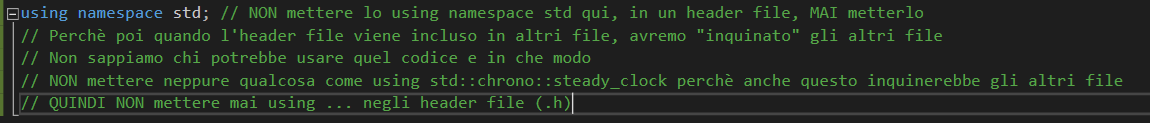
\includegraphics[width=1.2\textwidth, height=1.2\textheight, keepaspectratio]{./imgs/MAI_mettere_USING_negli_header_files.png}
	\caption{Mai mettere using in un header file}
	\label{fig:never_using_in_header}
\end{figure}

\textsf{\small Quindi, meglio mettere \textbf{using namespace} nei files \textbf{.cpp}, ma in generale, come abbiamo detto prima è meglio \textbf{non} utilizzarli.} \\

\textsf{\small Quindi \textbf{non} mettere \textbf{using namespace} in un header file, neanche \textbf{using namespace std}.} \\

% -------------------------- SECTION: STRUTTURE --------------------------------------

\newpage

\section{Strutture}

\textsf{\small \textbf{Definizione: } Le strutture sono dei tipi di dati definiti dall'utente per raggruppare oggetti di tipi diversi.} 

\textsf{\small Sono usati per rappresentare un record.}

\textsf{\small La keyword \textbf{struct} è usata per creare una struttura.}

\textsf{\small In questo modo semplicemente creiamo la struttura, ma non instanziamo nessun oggetto, per creare una istanza servirà richiamare il nome della struttura e poi il nome dell'istanza.}

\textsf{\small Per accedere ai campi della struttura si potrà usare l'operatore \textbf{.} (punto).}

\begin{lstlisting}
	struct nome_struttura{
		// campi della struttura
		int x;
		double d;
		char stringa[128];
	}; // Da notare il ; alla fine

	// Esempio una struttura per immagazzinare le coordinate di un punto.
	struct Point {
		int x;
		int y;
	};

	// In realtà in C++ non è necessario usare la keyword struct per creare un'istanza, a differenza del C.
	struct Point p1;
	p1.x = 0;
	p1.y = 1;
\end{lstlisting}

\textsf{\small In realtà in C++ non è necessario usare la keyword struct per creare un'istanza, a differenza del C.}

\textsf{\small Inoltre è anche possibile assegnare dei valori di default ai campi della struttura.} \\

\begin{lstlisting}
	struct Point{
		int x = 0;
		int y = 1;
	};

	struct Point p1;
	std::cout << p1.x << std::endl; // Output : 0
	std::cout << p1.y << std::endl; // Output : 1
\end{lstlisting}

\subsection{typedef}

\textsf{\small \textbf{Definizione: } La keyword \textbf{typedef} è usata essenzialmente per rinominare una tipologia.}

\textsf{\small Possiamo usare la parola chiave \textbf{typedef} per evitare di scrivere ogni volta struct nome\_della\_struttura per instanziare:} \\

\begin{lstlisting}
	typedef struct Point Punto;
	// Ora possiamo semplicemente scrivere Punto nome\_della\_istanza per creare una nuova istanza, al posto di dover scrivere struct Point nome\_della\_istanza.
	// In questo caso, potrebbe non sembrare molto, ma per strutture con nomi più lunghi è una manna dal cielo.
	
	Punto p1;
	p1.x = 3;
	p1.y = 2;
\end{lstlisting}

\textsf{\small Inoltre, ci sono diversi modi per creare una struttura apparte il modo visto prima, due di questi è attraverso il \textbf{typedef}: } \\

\begin{lstlisting}
	// Altro modo 1
	typedef struct Point {
		int x;
		int y;
	} Point;

	Point p1;
	p1.x = 1;
	p1.y = 0;
	
	// Altro modo 2
	struct Point {
		int x;
		int y;
	} typedef Point;

	Point p1;
	p1.x = 4;
	p1.y = 5;
\end{lstlisting}

\subsection{Funzioni nelle strutture} %TODO: oppure come subsection delle differenze C e C++

\textsf{\small A differenza del C, nelle strutture del C++ è possibile inserire delle funzioni.} \\

\begin{lstlisting}
	struct Rettangolo{
		int x;
		int y;
		int area(){
			return x * y;
		}
	};

	int main()
	{
		typedef struct Rettangolo Rettangolo;
		Rettangolo r1;
		r1.x = 3;
		r1.y = 2;
		std::cout << "Area rettangolo: " << r1.area() << std::endl; // Output : Area rettangolo: 6
		return 0;
	}
\end{lstlisting}

\subsection{Strutture nelle strutture}

\textsf{\small È possibile includere delle strutture all'interno di una struttura, come una matriosca.} \\

\begin{lstlisting}
	struct Point {
		int x;
		int y;
	};

	// Ovviamente la definizione della struttura Point deve essere fatta prima della struttura Rettangolo se la vogliamo includere in Rettangolo.
	struct Rettangolo{
		Point p;
		int area(){
			return p.x * p.y;
		}
	};

	typedef struct Rettangolo Rettangolo;
	Rettangolo r1;
	r1.p.x = 3;
	r1.p.y = 2;
	std::cout << "Area rettangolo: " << r1.area() << std::endl; // Output : Area rettangolo: 6
\end{lstlisting}

\subsection{Puntatore ad una struttura}

\textsf{\small È possibile far puntare un puntatore ad una struttura.} \\

\textsf{\small Per assegnare un valore ad uno specifico campo della struttura possiamo sia avvalerci dell'operatore \textbf{.} sia dell'operatore \textbf{->} che in questo caso fa esattamente la stessa cosa.} \\

\begin{lstlisting}
	struct Book {
		char  title[50];
		char  author[50];
		char  subject[100];
		int   book_id;
	};

	typedef struct Book Book;
	Book *pBook;
	
	// Possiamo sia fare così..
	(*pBook).title = "Learn C++";
	
	//.. sia fare così
	pBook->title = "Learn C++";
\end{lstlisting}

\subsection{Array di Strutture}

\textsf{\small Ovviamente è possibile creare un array di strutture, dove ogni elemento dell'array è una struttura.} \\

\begin{lstlisting}
	struct Cliente{
		int id;
		char nome[128];
	};

	typedef struct Cliente Cliente;
	
	Cliente clienti[2] = {{0, "Gigi"}, {1, "Pippo"}};
	// Oppure
	clienti[0].id = 0;
	clienti[0].nome = "Gigi";
	
	clienti[1].id = 1;
	clienti[1].nome = "Pippo";
	
	// Oppure si potrebbe anche fare così
	struct Cliente{
		int id;
		char nome[128];
	}cliente1, cliente2;

	cliente1.id = 0;
	cliente1.nome = "Gigi";
	
	cliente2.id = 1;
	cliente2.nome = "Pippo";
	
\end{lstlisting}

\subsection{Strutture come parametri e come ritorno}

\textsf{\small Ovviamente, si possono passare anche le strutture come parametri. Da fare attenzione che se non serve, meglio non copiare un'intera struttura quando la si passa come parametro.}

\begin{lstlisting}
	struct Book {
		char  title[50];
		char  author[50];
		char  subject[100];
		int   book_id;
	};
	
	void stampaLibro(struct Book* book){
		std::cout << "Titolo: " << book->title << std::endl;
		std::cout << "Autore: " << book->author << std::endl;
		std::cout << "Soggetto: " << book->subject << std::endl;
		std::cout << "Id: " << book->book_id << std::endl;
	}

	struct Book book1;
	std::strcpy( book1.title, "Learn C++ Programming");
	std::strcpy( book1.author, "Chand Miyan"); 
	std::strcpy( book1.subject, "C++ Programming");
	book1.book_id = 3;
	
	stampa(&book1);
	// Output : Titolo: Learn C++ Programming
	// Output : Autore: Chand Miyan
	// Output : Soggetto: C++ Programming
	// Output : Id: 3
\end{lstlisting}

\textsf{\small Al tempo stesso, si possono restituire strutture dalle funzioni.} \\

\begin{lstlisting}
	#define MATERIE 3
	
	struct studente{
		int matricola;
		char nome[128];
		char cognome[128];
		int voti[MATERIE];
		int media;
	};

	typedef struct studente Studente;
	
	// std::cin serve per l'input dell'utente.

	Studente createStudente(){
		Studente s;
		std:: cout << "Inserisci matricola: \n";
		std::cin >> s.matricola;
		
		std:: cout << "Inserisci nome: \n";
		std::cin >> s.nome;
		
		std:: cout << "Inserisci cognome: \n";
		std::cin >> s.cognome;
		
		int sum = 0;
		
		for(int i = 0; i < MATERIE; i++){
			std:: cout << "Inserisci voto: \n";
			std::cin >> s.voti[i];
			sum += s.voti[i];
		}
	
		s.media = sum / MATERIE;
		
		return s;
	}

	int main()
	{
		Studente s = createStudente();
		// Output : quelli inseriti
		std::cout << "Nome: " << s.nome << std::endl;
		std::cout << "Cognome: " << s.cognome << std::endl;
		std::cout << "Voto1: " << s.voti[0] << std::endl;
		std::cout << "Voto2: " << s.voti[1] << std::endl;
		std::cout << "Voto3: " << s.voti[2] << std::endl;
		std::cout << "Media: " << s.media << std::endl;
		return 0;
	}
\end{lstlisting}

\subsection{Strutture in C vs in C++}

\begin{tabular}{|c|c|}
	\hline
	\textbf{Strutture in C} & \textbf{Strutture in C++} \\
	\hline
	\textsf{\small Sono permessi solo membri dati, non funzioni.} & \textsf{\small Sono permessi sia dati sia funzioni membri.} \\
	\hline
	\textsf{\small Non può avere membri statici.} & \textsf{\small Può avere membri statici.} \\
	\hline
	\textsf{\small Non possiamo avere un costruttore.} & \textsf{\small Possiamo avere un costruttore.} \\
	\hline
	\textsf{\small L'inizializzazione diretta dei membri non è possibile.} & \textsf{\small L'inizializzazione diretta dei membri è possibile.} \\
	\hline
	\textsf{\small È necessario usare la keyword struct } & \textsf{\small Non è necessario usare la keyword struct.} \\
	\textsf{\small per dichiarare una variabile di tipo struct.} & \textsf{\small } \\
	\hline
	\textsf{\small Non supporta access modifiers.} & \textsf{\small Supporta gli access modifiers. } \\
	\textsf{\small } & \textsf{\small (public, private, protected, ecc..)} \\
	\hline
	\textsf{\small Sono permessi soltanto i puntatori alle strutture.} & \textsf{\small Sono permessi sia i puntatori sia le references.} \\
	\hline
	\textsf{\small L'operatore sizeof() genererà 0 } & \textsf{\small L'operatore sizeof() genererà 1 } \\
	\textsf{\small per una struttura vuota.} & \textsf{\small per una struttura vuota.} \\
	\hline
	\textsf{\small Il Data Hiding non è possibile.} & \textsf{\small Il Data Hiding è possibile.} \\
	\hline
\end{tabular}

% -------------------------- SECTION: UNION ------------------------------------------

\section{Union}

\textsf{\small \textbf{Definizione: } La \textbf{union} è un tipo di struttura dove l'ammontare di memoria è una fattore chiave.} \\

\begin{itemize}
	\item \textsf{\small Come le strutture, le union possono contenere diversi tipologie di variabili.}
	\item \textsf{\small Ogni qualvolta che una nuova variabile è inizializzata dall'union in C sovrascrive quella vecchia, ma in C++ usiamo quella locazione di memoria e non abbiamo bisogno di quella parola chiave.}
	\item \textsf{\small È utile quando i dati passati ad una funzione sono sconosciuti, utilizzare una \textbf{union} che contiene tutti i possibili tipi può essere il rimedio a questo problema.}
	\item \textsf{\small Utilizziamo la keyword \textbf{union} per crearne una.}
\end{itemize}

\begin{lstlisting}
	union nome_della_union {
		// tipi di dati
	}; // Da notare il ; proprio come nelle strutture.

	union var {
		int iVar;
		char cVar;
		float fVar;
	};

	int main()
	{
		// In C++ non serve la keyword union.
		union var V1, V2, V3;
		
		V1.iVar = 33;
		V2.cVar = 33;
		V3.fVar = 33.33;
		
		std::cout << "V1 var: " << V1.iVar << std::endl; // Output : V1 var: 33
		std::cout << "V2 var: " << V2.cVar << std::endl; // Output : V2 var: !
		std::cout << "V3 var: " << V3.fVar << std::endl; // Output : V3 var: 33.33
		
		return 0;
	}
\end{lstlisting}

\subsection{structure vs union}

\begin{tabular}{|c|c|}
	\hline
	\textbf{Structure} & \textbf{Union} \\
	\hline
	\textsf{\small Usa la keyword \textbf{struct}} & \textsf{\small Usa la keyword \textbf{union}}\\
	\hline
	\textsf{\small Quando una variabile è associata con una struttura} & \textsf{\small Quando una variabile è associata con } \\
	\textsf{\small il compilatore alloca la memoria } & \textsf{\small una union il compilatore alloca memoria } \\
	\textsf{\small per ogni membro.} & \textsf{\small considerando lo spazio occupato } \\
	\textsf{\small Lo spazio occupato dalla struttura} & \textsf{\small dal membro più grande.} \\
	\textsf{\small è maggiore o uguale alla somma} & \textsf{\small } \\
	\textsf{\small dello spazio dei suoi membri.} & \textsf{\small } \\
	\hline
	\textsf{\small Per ogni membro della struttura} & \textsf{\small La memoria allocata} \\
	\textsf{\small è assegnato uno spazio di allocazione unico.} & \textsf{\small è condivisa con i membri individuali dalla union.} \\
	\hline
	\textsf{\small Modificare un membro della struttura} & \textsf{\small Modificare un membro della union} \\
	\textsf{\small non modificherà gli altri membri.} & \textsf{\small modificherà gli altri membri.} \\
	\hline
	\textsf{\small I membri individuali possono essere} & \textsf{\small Solo un membro alla volta} \\
	\textsf{\small acceduti ad ogni momento.} & \textsf{\small può essere acceduto.} \\
	\hline
	\textsf{\small Si possono inizializzare } & \textsf{\small Solo il primo membro} \\
	\textsf{\small diversi membri alla volta.} & \textsf{\small della union può essere inizializzato.} \\
	\hline
\end{tabular}

% -------------------------- SECTION: CLASSI -----------------------------------------

\newpage

\section{Classi}

\textsf{\small \textbf{Definizione: } La \textbf{classe} è il concetto fondamentale, il muro portante, la pietra miliare della programmazione ad oggetti. È un tipo di dato definito dall'utente che contiene i propri membri dati e membri funzioni che possono essere acceduti creando un'istanza.} \\ %TODO: Non mi sembra si dica il muro portante.

\textsf{\small Una classe è come uno stampino, un modello per creare oggetti. } \\

\textsf{\small È la differenza sostanziale del C++ con il C, l'avere le classi rendendo il linguaggio: un linguaggio a programmazione di oggetti. } \\ %TODO: questa la portrei riscrivere meglio.

\textsf{\small Ogni classe rappresenta un oggetto che possiede degli attributi, delle caratteristiche (dati) e dei comportamenti stabiliti dalle funzioni che possiede. } \\

\begin{figure}[ht]
	\centering
	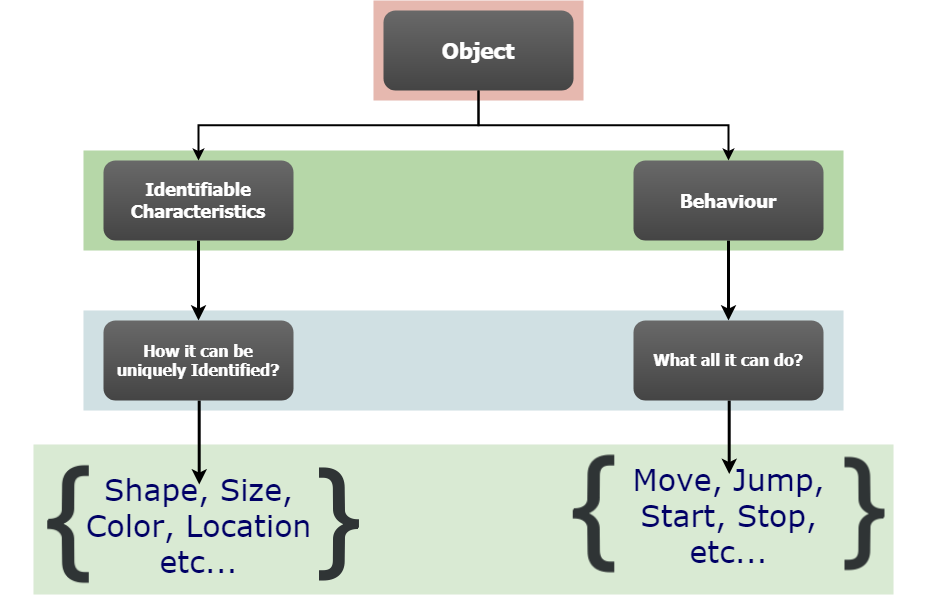
\includegraphics[width=1\textwidth, height=1\textheight, keepaspectratio]{./imgs/class_data_and_behaviour.png}
	\caption{Dati e comportamenti di una classe}
	\label{fig:class_data_and_behaviour}
\end{figure}

\textsf{\small Per creare una classe si utilizza la keyword \textbf{class}. Lo spazio di memoria non è allocata quando la classe viene definita, ma quando viene istanziata. } \\

\textsf{\small Per creare un'istanza della classe, si chiama il nome della classe e poi il nome dell'istanza.} \\

\subsection{Costruttori e Distruttori}

\subsubsection{Costruttori}

\textsf{\small \textbf{Definizione: } Il \textbf{costruttore} è una speciale funzione membro (della classe) che inizializza gli oggetti di una classe. Il costruttore è chiamato automaticamente quando un'istanza della classe viene creata. È una funzione speciale perché non tipi di ritorno, o meglio il tipo di ritorno è la classe stessa. } \\ %Funzione membro o membra?

\textsf{\small Il nome di questa funzione \textbf{costruttore} è identico al nome della classe stessa.} \\

\textsf{\small Se non specifichiamo un \textbf{costruttore}, uno di default verrà creato dal compilatore (senza parametri e con il corpo della funzione vuoto).} \\

\subsubsection{Initialization List}

\textsf{\small \textbf{Definizione: } La \textbf{Initialization List} è usata per inizializzare i dati membri della classe. Per fare questo aggiungiamo un \textbf{:} (due punti) dopo il costruttore e inizializziamo le variabili e le separiamo da delle virgole.} \\

\textsf{\small Può essere utile per:}

\begin{itemize}
	\item \textsf{\small Chiamare il costruttore della classe base.}
	\item \textsf{\small Inizializzare i membri prima che il costruttore venga eseguito.}
	\item \textsf{\small Per inizializzare i membri const non statici.}
	\item \textsf{\small Per inizializzare dei membri referenze}
	\item \textsf{\small Per inizializzare gli oggetti membri che non hanno un default constructor.}
	\item \textsf{\small Per inizializzare i membri della classe base.}
	\item \textsf{\small Quando il nome del costruttore è lo stesso del dato.}
	\item \textsf{\small Per questioni di performance.}
	%\item \textsf{\small }
\end{itemize}

\begin{lstlisting}
	// Questo codice non andrebbe, perché mVal è const. Non possiamo cambiare il valore di una const nel costruttore perché è segnato come const.
	class Demo {
			// Costruttore
			Demo(int& val)
			{
				mVal = val;
			}
		
			const int& mVal;
	};

	// Questo invece è possibile:
	class Demo {
			// Quindi puoi usare la lista di inizializzazione per fare questo.
			// Costruttore : inizialization list
			Demo(int& val) : mVal(val)
			{
			}
		
			const int& mVal;	
	};
\end{lstlisting}

\subsubsection{Distruttori}

\textsf{\small \textbf{Definizione: } Il \textbf{distruttore}, come dice la parola, è una funzione membro della classe che viene invocata automaticamente quando un oggetto (istanza della classe) viene distrutto/eliminato. Il che significa che il distruttore è l'ultima funzione ad essere chiamata. } \\

\textsf{\small Per definire un \textbf{distruttore} si crea una funzione con lo stesso nome della classe, ma prima del nome deve essere accompagnata dal simbolo \textbf{~} (tilde).} \\

\subsubsection{Proprietà del distruttore}

\begin{itemize}
	\item \textsf{\small Il distruttore è invocato automaticamente quando gli oggetti sono distrutti.}
	\item \textsf{\small Non può essere dichiarato \textbf{static} o \textbf{const}.}
	\item \textsf{\small Il \textbf{distruttore} non ha argomenti.}
	\item \textsf{\small Non ha tipi di ritorno, nemmeno \textbf{void}.}
	\item \textsf{\small Un oggetto della classe con un distruttore non può diventare membro di una \textbf{union}.}
	\item \textsf{\small Un distruttore dovrebbe essere dichiarato nella sezione \textbf{public}.}
	\item \textsf{\small Il programmatore non può accedere all'indirizzo del \textbf{distruttore}.}
	%\item \textsf{\small }
\end{itemize}

\subsubsection{Quando viene chiamato il distruttore?}

\begin{itemize}
	\item \textsf{\small La funzione finisce.}
	\item \textsf{\small Il programma termina.}
	\item \textsf{\small Un blocco contenente le variabili cessa.}
	\item \textsf{\small Un operatore \textbf{delete} viene chiamato.}
\end{itemize}

\begin{lstlisting}
	class MyClass {
		// Costruttore
		MyClass(){
			// Corpo del costruttore.
		}
		// Distruttore
		~MyClass(){
			// Corpo del distruttore.
		}
	}
\end{lstlisting}

\subsection{Access modifiers}

\textsf{\small \textbf{Definizione: } Gli \textbf{Access Modifiers} in una classe sono usati per assegnare l'accessibilità ai membri della classe. Questo permette una importante feature della programmazione ad oggetti, ovvero la \textbf{Data Hiding} che permette di prevenire l'accesso diretto dei dati da parte delle funzioni del programma.} \\

\textsf{\small Ci sono 3 tipi di \textbf{access modifiers}:} \break

\begin{tabular}{|c|c|}
	\hline
	\textbf{Access Modifier} & \textbf{Definizione} \\
	\hline
	\textsf{\small \textbf{public}} & \textsf{\small accessibile a tutti.} \\
	\hline
	\textsf{\small \textbf{private}} & \textsf{\small accessibile solo all'interno della classe stessa.} \\
	\hline
	\textsf{\small \textbf{protected}} & \textsf{\small accessibile solo alla classe, alle sue sottoclassi (ereditarietà)} \\
	\textsf{\small } & \textsf{\small ed alle classi amiche (friend class).} \\
	\hline
\end{tabular}

\subsubsection{Incapsulamento}

\textsf{\small \textbf{Definizione: } L'\textbf{incapsulamento} è un concetto di programmazione ad oggetti che mette assieme i dati e le funzioni che manipolano i dati per mantenerli sicuri da interferenze esterne e da un uso improprio.} \\

\textsf{\small L'\textbf{incapsulamento} dei dati è un meccanismo di impacchetamento di dati e delle funzioni che li usano. } \\

\textsf{\small La \textbf{Data abstraction} è un meccanismo che espone solo le interfacce e nasconde  i dettagli dell'implementazione dall'utente.} \break

%TODO: qui fare un esempio concreto.

\begin{lstlisting}
	class Sommatore {
		// con public sono accessibili da tutti.
	  public:
		// Costruttore.
		Sommatore(int i = 0){ // i = 0 vuol dire che assegniamo un valore di default, casomai l'utente non voglia inserirne uno.
			totale = i;
		}
	
		// Interfaccia al mondo esterno.
		void aggiungiNumero(int numero){
			totale += numero;
		}
	
		// Interfaccia al mondo esterno.
		int getTotale(){
			return totale;
		}
	
	private:
		// Dati nascosti al mondo esterno.
		int totale;
	};

	int main(){
		Sommatore s;
		
		s.aggiungiNumero(3);
		s.aggiungiNumero(6);
		s.aggiungiNumero(9);
		
		std::cout << "Totale: " << s.getTotale() << std::endl; // Output: Totale: 18
		return 0;
	}
\end{lstlisting}

%TODO: operatore :: (due punti)

\subsection{scope resolution operator ::}

\textsf{\small L'operatore \textbf{scope resolution} indicato con i \textbf{::} (doppi due punti) può essere usato per definire delle funzioni della classe fuori dalla stessa.} \\

\textsf{\small Può essere usato per accedere ad una variabile globale quando c'è anche una variabile locale con lo stesso nome.} \\

\textsf{\small Può essere usato quando si ha la definizione di una classe all'interno di un'altra classe.} \\

\begin{lstlisting}
#include <iostream>
int weight = 33;
	
class MyClass {
	public:
		MyClass(){
			num = 66;
		}	
	
		void display();
		
		int get_num(){
			return num;
		}
	
	private:
		int num;
};

void MyClass::display(){
	std::cout << "Il valore di num e\': " << get_num() << std::endl;
}

int main(){
	int weight = 99;
	MyClass istanza;
	istanza.display(); // Output: Il valore di num è: 66
	
	std::cout << "Valore della variabile weight locale: " << weight << std::endl;
	std::cout << "Valore della variabile globale: " << ::weight << std::endl; 
	return 0;
}
\end{lstlisting}

\subsection{Getters \& Setters}

\textsf{\small Per via dell'incapsulamento, per poter recuperare (getter) o impostare (settare) le variabili private usufruiamo dei \textbf{getters \& setters} che sono due funzioni, una per recuperare il dato (getter) e l'altro per impostarlo (setter).} \\

\begin{lstlisting}
	class MyClass {
	public:
		MyClass(){
			// Costruttore
		}
	
		// Recupera il valore della variabile number.
		int get_number(){
			return number;
		}
		
		// Imposta un nuovo valore alla variabile number.
		void set_number(int number_t){
			number = number_t;
		}
	
	private:
		int number;
	};
\end{lstlisting}

\subsection{Ereditarietà}

\textsf{\small \textbf{Definizione: } L'\textbf{ereditarietà} è la capacità di derivare le proprietà e le caratteristiche da un'altra classe. È una delle feature più importanti della programmazione ad oggetti.} \\

\textsf{\small La classe che deriva è chiamata \textbf{derived class} o \textbf{sub class}, mentre quella che viene derivata è chiamata \textbf{base class} o \textbf{super class}.} \\

\textsf{\small Per implementare l'ereditarietà usiamo l'operatore \textbf{:} quando andiamo a definire la classe derivata. Questa è chiamata la \textbf{initialization list} serve per chiamare la classe base e per inizializzare le variabili membri prima che il costruttore venga eseguito.} \\

\begin{lstlisting}
	class nome_classe_derivata : modalità_di_accesso nome_classe_base {
		// Corpo della subclass/ derived class
	}
\end{lstlisting}

\begin{figure}[ht]
	\centering
	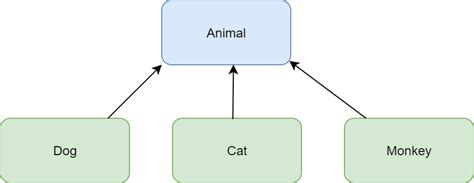
\includegraphics[width=1\textwidth, height=1\textheight, keepaspectratio]{./imgs/animal_class_uml.jpg}
	\caption{Concetto dell'ereditarietà}
	\label{fig:ereditarietà2}
\end{figure}

%TODO: aggiungere classe Monkey
\begin{lstlisting} 
	class Animal {
	public:
		Animal(){
			std::cout << "Animal Constructor" << std::endl;
		}
	
		void eat(){
			std::cout << "gnam gnam.." << std::endl;
		}
	
		void sleep(){
			std::cout << "Sleeping zzz.." << std::endl;
		}
	};

	class Dog : public Animal {
	public:
		Dog(std::string name, int weight){
			std::cout << "Dog Constructor" << std::endl;
			// Qui stiamo assegnando i valori dei parametri alle nostre variabili nella classe (quelle in private).
			// Per evitare confusioni potremmo anche chiamare i parametri del costruttore in maniera diversa (tipo: nomeparametro\_t per differenziarlo oppure \_nomeparametro) oppure per differenziare le variabili della classe potremmo aggiungerci la keyword this.
			name = name;
			weight = weight;
		}
	
		void bark(){
			std::cout << "Wuuf Wuuf" << std::endl;
		}
	
		std::string get_name(){
			return name;
		}
	
		int get_weight(){
			return weight;
		}
	
	private:
		std::string name;
		int weight;
	};

	class Cat : public Animal {
		public:
		Cat(std::string name, int weight){
			std::cout << "Cat Constructor" << std::endl;
			// Qui usiamo il puntatore this per far riferimento alle variabili membre della classe al posto di quelle passate come parametro al costruttore.
			this->name = name;
			this->weight = weight;
		}
		
		void meow(){
			std::cout << "Meow Meow" << std::endl;
		}
	
		std::string get_name(){
			return name;
		}
		
		int get_weight(){
			return weight;
		}
		
		private:
		std::string name;
		int weight;
	};

	int main(){
		Dog floki {"floki", 36};
		std::cout << floki.bark() << std::endl;
		std::cout << floki.get_name() << std::endl;
		std::cout << floki.get_weight() << std::endl;
		
		// Output: Animal Constructor
		// Output: Dog Constructor
		// Output: floki
		// Output: 36
		return 0;
	}
\end{lstlisting}

\begin{figure}[ht]
	\centering
	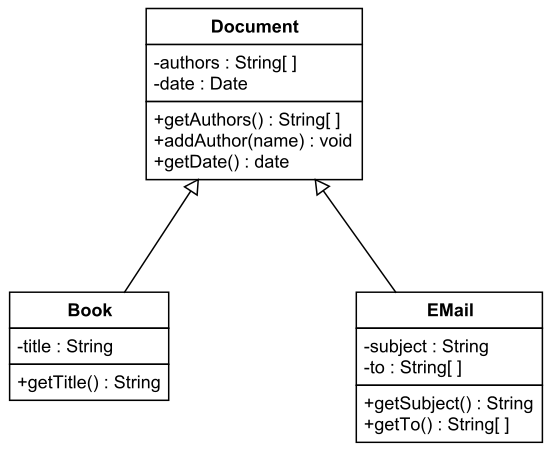
\includegraphics[width=1\textwidth, height=1\textheight, keepaspectratio]{./imgs/inheritance_class_uml2.jpg}
	\caption{Ereditarietà in un diagramma UML}
	\label{fig:ereditarietà}
\end{figure}

\subsubsection{this pointer}

\textsf{\small \textbf{Definizione: } La keyword \textbf{this} serve per riferirsi all'oggetto in cui ci troviamo.} \\ %TODO: da rivedere, aggiungere esempio, ecc..

\subsection{Multi-Ereditarietà}

%TODO: diamond problem: ambiguity, classe che deriva da due classi che entrambe derivano dalla stessa base class?

\textsf{\small Il c++ permette l'\textbf{ereditarietà multipla}, quindi una classe può derivare da più classi base. Non è presente invece l'implementazione di interfacce.} \\

\begin{lstlisting}
	class A
	{
		public:
		A()  { cout << "A's constructor called" << endl; }
	};
	
	class B
	{
		public:
		B()  { cout << "B's constructor called" << endl; }
	};
	
	class C: public B, public A  // Da notare l'ordine.
	{
		public:
		C()  { cout << "C's constructor called" << endl; }
	};
	
	int main()
	{
		C c;
		// Output: B's constructor called
		// Output: A's constructor called
		// Output: C's constructor called
		return 0;
	}
\end{lstlisting}

\subsection{Forward Declaration}

\textsf{\small \textbf{Definizione: } La \textbf{forward declaration} è quando prima dichiariamo una funzione, una classe, eccetera.. con la premessa che da qualche parte nel codice più in là ci sarà una definizione di questa funzione, classe, eccetera..} \\

\textsf{\small Può essere utile per aiutare il compilatore per assicurarsi che non ci sono stati errori di spelling o di numero sbagliato di argomenti da passare.} 

\textsf{\small Può essere utile per ridurre il tempo di \emph{build} del programma.}

\textsf{\small Può essere utile per rompere il ciclo delle referenze dove due definizioni si usano a vicenda.} \\

\begin{figure}[H]
	\centering
	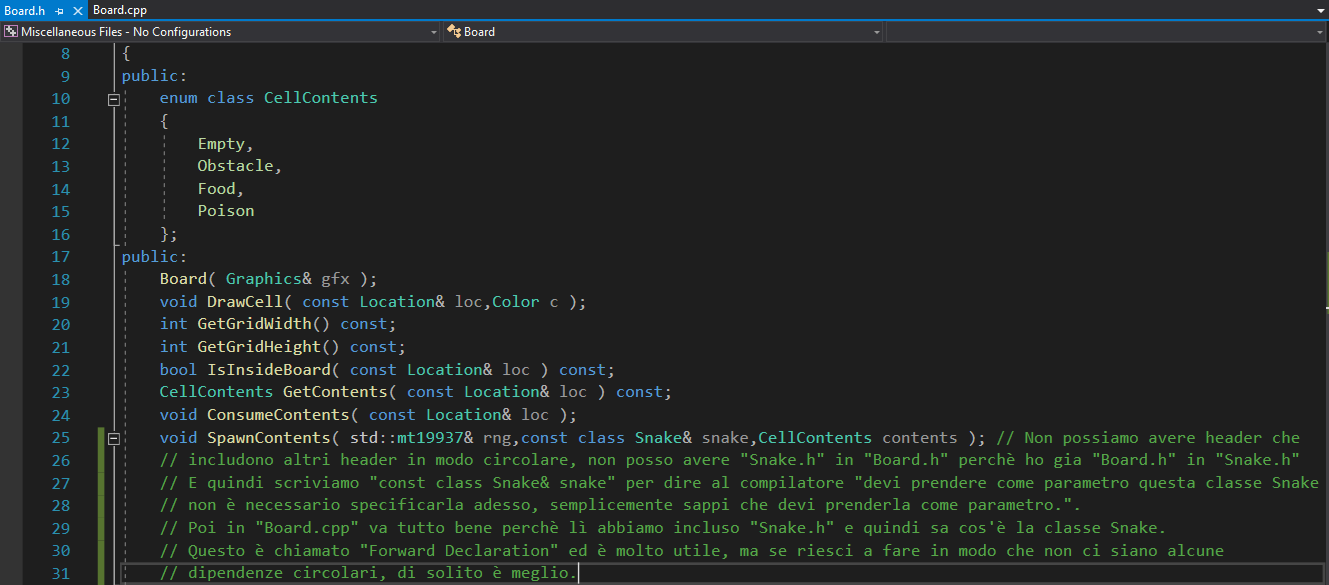
\includegraphics[width=1.2\textwidth, height=1.2\textheight, keepaspectratio]{./imgs/Forward_declaration.png}
	\caption{Forward Declaration}
	\label{fig:forward_declaration}
\end{figure}

%TODO: aggiungere il resto del codice dell'immagine potrebbe essere utile

\subsection{Chiamata a funzione statica e a membro} 

\subsubsection{Static nelle Classi}

\textsf{\small \textbf{Definizione: } Possiamo definire un membro della classe statica attraverso la keyword \textbf{static}. Questo significa che non importa quante istanze della classe vengano create, c'è una sola copia del membro statico.}

\textsf{\small Un membro statico è condiviso da tutti gli oggetti della classe. Se non è presente un'inizializzazione al membro statico, il suo valore di default sarà 0.} \\ 

\textsf{\small Per accedere a questa funzione statica o membro o altro \textbf{non} possiamo utilizzare l'operatore \textbf{.}, ma dobbiamo usufruire dell'operatore \textbf{::}.} \\

\begin{lstlisting}
class MyClass {
	public:
		MyClass(){
			// Costruttore
		}	
	
		// Questo è un esempio, non ho messo l'implementazione della funzione.
		static int calcola_qualcosa() {};
};

int main(){
	MyClass oggetto;
	// Non posso fare oggetto.calcolaQualcosa();
	// Devo fare MyClass::calcola\_qualcosa();
	MyClass::calcola_qualcosa();
	return 0;
}
\end{lstlisting}

\begin{figure}[H]
	\centering
	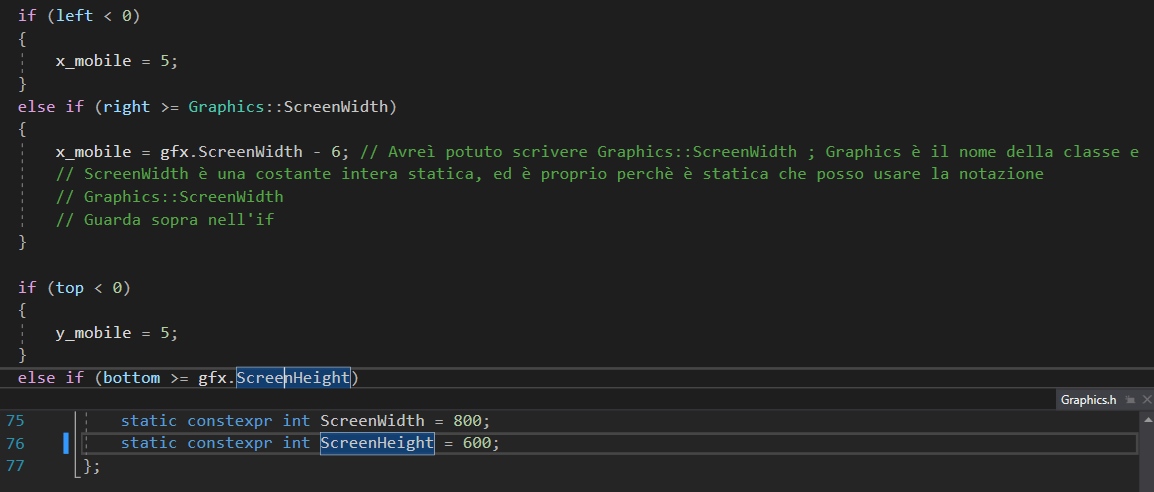
\includegraphics[width=1.2\textwidth, height=1.2\textheight, keepaspectratio]{./imgs/Class__static_type2.png}
	\caption{Chiamata a membro statico}
	\label{fig:class_static_type}
\end{figure}

\subsection{Funzioni e la keyword const}

\textsf{\small Ci sono vari significati che la keyword \textbf{const} assume e fa assumere alla funzione quando si trova in essa.} \\

\textsf{\small Mettendo \textbf{const} nei parametri della funzione, ciò significa che i parametri di quella funzione non possono essere cambiati, perché sono costanti.}

%TODO: esempio

%TODO: const come return type.

\begin{figure}[H]
	\centering
	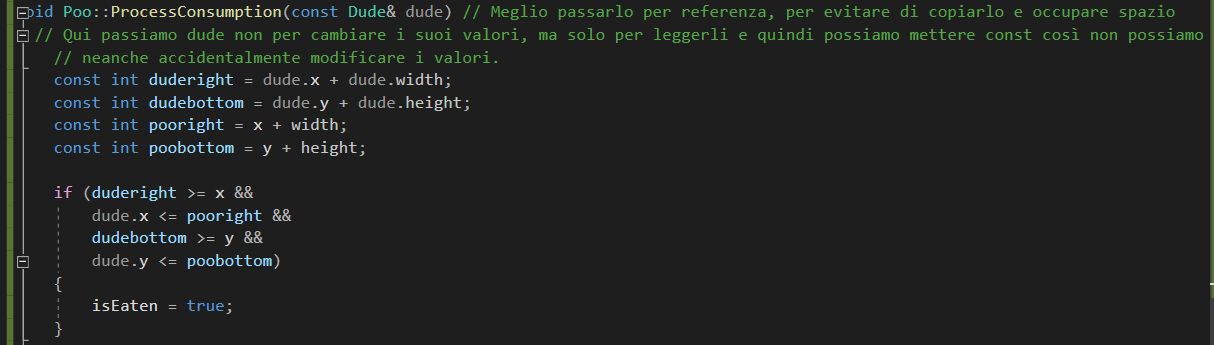
\includegraphics[width=1.2\textwidth, height=1.2\textheight, keepaspectratio]{./imgs/const_as_parameter.png}
	\caption{Const come parametro}
	\label{fig:const_as_parameter}
\end{figure}

\textsf{\small Mentre, la keyword \textbf{const} alla fine della funzione (Const member function in inglese) significa che l'oggetto chiamato da questa funzione non può essere modificato, questo previene modifiche accidentali all'oggetto. } \\

\begin{lstlisting}
	int val = 5;
	
	// Se aggiungessimo una riga per modificare il valore, otterremmo un errore.
	// Inoltre mettere quel const lì esprime l'intento di non cambiare l'oggetto 
	// della funzione.
	int getValue() const
	{
		return val;
	}
\end{lstlisting}

\begin{figure}[H]
	\centering
	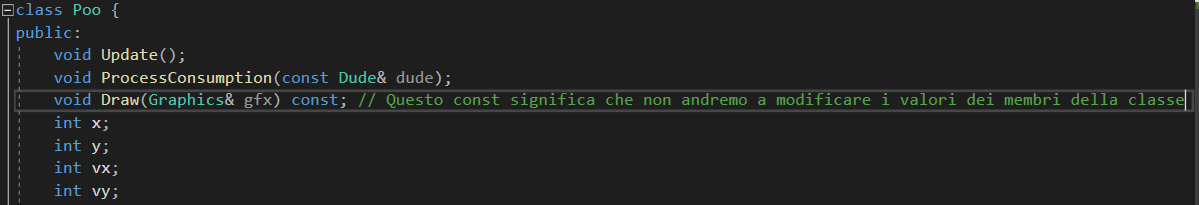
\includegraphics[width=1.2\textwidth, height=1.2\textheight, keepaspectratio]{./imgs/const_function_class_members.png}
	\caption{Const function class members}
	\label{fig:const_function_class_members}
\end{figure}

\textsf{\small Infine, c'è restituire \textbf{const} come valore di ritorno di una funzione, ma non sembra di molta utilità, tranne per le move-semantics, per lo meno se lo si ritorna per valore, mentre ritornarlo per reference protegge il valore di ritorno dall'essere modificato.} \\

\subsection{Class vs Struct}

\textsf{\small In C++ le classi e le strutture sono simili, ma con alcune differenze:} \break

\begin{tabular}{|c|c|}
	\hline
	\textbf{Class} & \textbf{Struct} \\
	\hline
	\textsf{\small I membri della classe sono privati da default.} & \textsf{\small I membri di una struttura sono pubblici da default.} \\
	\hline
	\textsf{\small L'allocazione della memoria avviene nell'heap.} & \textsf{\small L'allocazione della memoria avviene sullo stack.} \\
	\hline
	\textsf{\small È un tipo di dato per referenza.} & \textsf{\small È un tipo di dato per valore.} \\
	\hline
	\textsf{\small Si dichiara usando la keyword \textbf{class}.} & \textsf{\small Si dichiara usando la keyword \textbf{struct}.} \\
	\hline
	%\textsf{\small } & \textsf{\small } \\
\end{tabular}

%TODO: costruttori, distruttori, copy, move, rule of 3, rule of 5. (rule of 7?); Forse alcune cose in un altro capitolo. (queste assieme al polimorfismo nel secondo capitolo).

%TODO: non usare la keyword new per istanziare?! e delete, magari subsections sulla new e la delete.

% -------------------------- SECTION: OPERATORS --------------------------------------

%\section{Operators}

%TODO: come creare operatori, però questo potrei metterlo in un altro capitolo, non qui nelle basi del linguaggio.

%TODO: aggiungere le Convenzioni del linguaggio.

% -------------------------- SECTION: CONVENZIONI ------------------------------------

\newpage

\section{Convenzioni del linguaggio}

\textsf{\small \textbf{Definizione: } Le \textbf{convenzioni} sono delle linee guida di un linguaggio che raccomandano un certo stile di programmazione. Queste permettono un codice più chiaro, più leggibile e rende il codice di un software più semplice da mantenere.} \\

\textsf{\small Inoltre, sia il codice che i commenti dovrebbero essere in inglese a differenza di come ho fatto io in questa guida.} \\

\textsf{\small Potete trovare tutte le convenzioni del linguaggio nelle \textbf{C++ Core Guidelines} : \href{https://github.com/isocpp/CppCoreGuidelines}{CppCoreGuidelines}} \\

\textsf{\small Qui anche una versione più corta (non ufficiale): \href{https://github.com/openbmc/docs/blob/master/cpp-style-and-conventions.md}{CppStyleAndConventions}} \\

\textsf{\small Comunque ne elencherò qualche d'una: } \break

\subsection{Generale}

\begin{itemize}
	\item \textsf{\small Lunghezza della riga limitata a 80 caratteri}
	\item \textsf{\small Indentazione con 4 spazi.}
	\item \textsf{\small I files dovrebbero usare le newlines stile Unix $\backslash n$.}
\end{itemize}

\subsection{Parentesi Graffe}

\textsf{\small Utilizzare \emph{Allman Style} brackets (parentesi). Le parentesi graffe sono sulla loro linea allo stesso livello con lo statement sopra.} \\

\begin{lstlisting}
	if (condition)
	{
	
	}
\end{lstlisting}

\textsf{\small Anche gli if con una sola linea dovrebbero avere le parentesi graffe.} \\

\subsection{Indentazione}

\textsf{\small Il contenuto in un \textbf{namespace} dovrebbe essere allo stesso livello di indentazione del namespace stesso. } \\

\textsf{\small Il contenuto in una \textbf{classe}, \textbf{struct}, \textbf{funzioni}, \textbf{if}, \textbf{loop}, \textbf{switch}, \textbf{cases} e \textbf{labels} (dei goto) dovrebbe essere indentato.} \\

\subsection{Convenzioni sui nomi}

\begin{itemize}
	\item \textsf{\small Non c'è nè prefisso nè suffisso a nessun nome.}
	\item \textsf{\small Gli acronimi dovrebbero essere dello stesso case.}
\end{itemize}

\begin{lstlisting}
	// Correct.
	SomeBMCType someBMCVariable = bmcFunction();
\end{lstlisting}

\subsection{Ordine Inclusione Header files}

\textsf{\small Inclusione degli headers in un header file:} \\

\begin{itemize}
	\item \textsf{\small headers locali}
	\item \textsf{\small librerie c}
	\item \textsf{\small librerie cpp}
\end{itemize}

\textsf{\small Inclusione degli headers in un source file (.cpp):} \\

\begin{itemize}
	\item \textsf{\small source.hpp (se applicabile)}
	\item \textsf{\small headers locali}
	\item \textsf{\small librerie c}
	\item \textsf{\small librerie cpp}
\end{itemize}

\textsf{\small In ordine alfabetico.} \\

\subsubsection{Files}

\begin{itemize}
	\item \textsf{\small Gli headers C++ dovrebbero finire in \emph{.hpp}. Gli headers C dovrebbero finire in \emph{.h}.}
	\item \textsf{\small I files dovrebbero essere chiamati nel modo (case) lower\_snake\_case.}
\end{itemize}

\subsection{Types}

\begin{itemize}
	\item \textsf{\small Preferire \emph{using} a \emph{typedef}.}
	\item \textsf{\small Le strutture, classi, enums dovrebbero essere tutti in UpperCamelCase.}
	\item \textsf{\small Preferire gli scope namespaces al posto di nomi con lunghi prefissi.}
	\item \textsf{\small Un alias di una singola parola con una struct / class dovrebbe essere in minuscolo, ma un alias a più parole dovrebbe essere UpperCamelCase.}
	\item \textsf{\small Eccezioni: Una libreria API potrebbe usare il modo lower\_snake\_case per accordarsi alle convenzioni STL o ad una libreria C. Application APIs dovrebbero tutte essere UpperCamelCase.}
	\item \textsf{\small Eccezione: Per convenienza un tipo di una classe template potrebbe finire in \_t per accordarsi alle convenzioni STL.}
	%\item \textsf{\small }
\end{itemize}

\subsection{Variabili}

\textsf{\small Le variabili dovrebbero tutte essere lowerCamelCase, inclusi i membri delle classi, senza underscore (trattini bassi).} \\

\subsection{Funzioni}

\begin{itemize}
	\item \textsf{\small Le funzioni dovrebbero essere lowerCamelCase.}
	\item \textsf{\small Eccezione: Una libreria API potrebbe usare lower\_snake\_case in accordo con le convenzioni STL o di una sottostante libreria in C che sta astraendo. Application API dovrebbero tutte essere lowerCamelCase.}
	%\item \textsf{\small }
\end{itemize}

\subsection{Costanti}

\begin{itemize}
	\item \textsf{\small Costanti e i membri delle enums dovrebbero essere chiamati come le variabili in lowerCamelCase.}
\end{itemize}

\subsection{Namespaces}

\begin{itemize}
	\item \textsf{\small I namespaces dovrebbero essere lower\_snake\_case.}
	\item \textsf{\small Top-level namespace dovrebbe essere chiamato sulla base della repository che lo contiene.}
	\item \textsf{\small Favorisci un namespace chiamato 'details' o 'internal' per indicare l'equivalente di un namespace 'private' in un header file e namespaces anonimi in un file C++.}
\end{itemize}

\subsection{Header Guards}

\textsf{\small Preferire \textbf{\#pragma} allo stile \textbf{\#ifndef}.}\\

\subsection{Spazi bianchi addizionali}

\begin{itemize}
	\item \textsf{\small Segui lo stile di dichiarazione del C++}
\end{itemize}

\begin{lstlisting}
	foo(T& bar, const S* baz); // Correct.
	foo(T &bar, const S *baz); // Incorrect.
\end{lstlisting}

\begin{itemize}
	\item \textsf{\small Usa gli spazi bianchi moderatamente.}
	\item \textsf{\small Inserisci uno spazio bianco prima e dopo if e loops.}
\end{itemize}

\begin{lstlisting}
	if (...)
	while (...)
	for (...)
\end{lstlisting}

\begin{itemize}
	\item \textsf{\small Aggiungi spazio bianco attorno agli operatori binari per leggibilità}
\end{itemize}

\begin{lstlisting}
	foo((a-1)/b,c-2); /// Incorrect.
	foo((a - 1) / b, c - 2); /// Correct.
\end{lstlisting}

\begin{itemize}
	\item \textsf{\small Non inserire spazi bianchi dopo gli operatori unari.}
\end{itemize}

\begin{lstlisting}
	a = * b;  /// Incorrect.
	a = & b;  /// Incorrect.
	a = b -> c;  /// Incorrect.
	if (! a)  /// Incorrect.
\end{lstlisting}

\begin{itemize}
	\item \textsf{\small Non inserire spazi bianchi nè prima nè dopo una chiamata a funzione e ai parametri.}
\end{itemize}

\begin{lstlisting}
	foo(x, y); /// Correct.
	foo ( x , y ); /// Incorrect.
	
	do (...)
	{
	} while(0); /// 'while' qui è strutturato come una chiamata a funzione.
\end{lstlisting}

\begin{itemize}
	\item \textsf{\small Preferire una linea a capo dopo gli operatori per mostrare la continuazione.}
\end{itemize}

\begin{lstlisting}
	if (this1 == that1 &&
	this2 == that2) /// Correct.
	
	if (this1 == that1
	&& this2 == that2) /// Incorrect.
\end{lstlisting}

\begin{itemize}
	\item \textsf{\small Le linee lunghe dovrebbero avere la continuazione che inizi allo stesso livello delle parentesi o tutti gli oggetti all'interno delle parentesi dovrebbero essere al secondo livello di indentazione.}
\end{itemize}

\begin{lstlisting}
	reallyLongFunctionCall(foo,
	bar,
	baz); // Correct.
	
	reallyLongFunctionCall(
	foo,
	bar,
	baz); // Also correct.
	
	reallyLongFunctionCall(
	foo, bar, baz); // Similarly correct.
	
	reallyLongFunctionCall(foo,
	bar,
	baz); // Incorrect.
\end{lstlisting}

\subsection{Linee Guida Miste}

\begin{itemize}
	\item \textsf{\small  Usare sempre size\_t o ssize\_t per cose come contatori, pesi, ecc.. C'è bisogno di un forte motivo razionale per usare un tipo come uint8\_t quando size\_t può fare lo stesso lavoro.}
	\item \textsf{\small Usa uint8\_t, int16\_t, uint32\_t, int64\_t quando è importante per l'interazione coll'hardware. Non usarli senza una buona motivazione, quando le interazioni coll'hardware non sono coinvolte; preferire size\_t o int piuttosto.}
\end{itemize}

% ------------------------------ FINE CAPITOLO ---------------------------------------
	
	% ----------------------------- CONCETTI INTERMEDI -----------------------------------

\chapter{Concetti Intermedi}

%Possibili argomenti aggiuntivi di questo capitolo: 

%TODO: inline functions.

%TODO: NULL (o null) vs nullptr

%TODO: explicit keyword, converting constructor.

%TODO: Private Destructor.

%TODO: copy elision.

%TODO: pure virtual destructors.

%TODO: SFINAE (Substitution Failure is Not An Error). nel chapter sugli algoritmi.

%TODO: sttrutture dati cosa sono? Strutture dati: array, linked list, stack, queue. E anche Abstract Data Types (ADT): list, stack, queue. map usa Red Black Tree.

%TODO: <functional>?

% -------------------------- SECTION: INTRODUZIONE -----------------------------------

\section{Introduzione}

\textsf{\small In questo capitolo, tratterò argomenti non necessariamente più complicati, ma che non considererei basi. } \\

\textsf{\small In questo capitolo vedremo ulteriori concetti riguardo le classi, il polimorfismo, le varie tipologie di costruttori, la programmazione generale, le lambdas, la programmazione funzionale e molto altro ancora..} \break

% -------------------------- SECTION: STL --------------------------------------------

%TODO: forse è quasi da mettere dopo i templates visto che bisogna sapere cosa sono i templates.

\section{STL | Standard Template Library}

\textsf{\small \textbf{Definizione: } La \textbf{Standard Template Library} (\emph{STL}) è un insieme di classi template che forniscono le classiche strutture dati e funzioni come: liste, stacks, arrays, eccetera..} \break

\textsf{\small È una libreria di contenitori (containers) di classi, algoritmi e iteratori. È una libreria generalizzata, i suoi componenti sono parametrizzati.} \\

\textsf{\small È stata sviluppata separatamente e poi sottoposta al \textbf{C++ standard commitee} per essere considerata e per dare loro la possibilità di adottarla nel linguaggio.} \break

\textsf{\small \textbf{L'STL ha quattro componenti: } } \\

\begin{itemize}
	\item \textsf{\small Algoritmi}
	\item \textsf{\small Contenitori}
	\item \textsf{\small Funzioni}
	\item \textsf{\small Iteratori}
\end{itemize}

\subsection{Che cos'è \#include <bits/stdc++.h>?}

\textsf{\small \textbf{Definizione: } È un header file che include tutti gli header files della \textbf{STL}.} \\

\textsf{\small \textbf{Non} dovrebbe essere usato perché: } \\

\begin{itemize}
	\item \textsf{\small è \emph{lazy} (pigro).}
	\item \textsf{\small è un header del compilatore \emph{GCC} e quindi \textbf{non} è portabile, ovvero potrebbe \textbf{non} andare in altri.}
	\item \textsf{\small non sai che cosa fa perché i suoi contenuti \textbf{non} sono standard.}
	\item \textsf{\small ogni header file dovrebbe essere \emph{parsato} il che renderebbe tutto più lento.}
	\item \textsf{\small rende il codice \textbf{non} portabile.}
\end{itemize}

% -------------------------- SECTION: TEMPLATES --------------------------------------

\newpage

\section{Templates}

\textsf{\small Immaginiamo di avere un codice, esempio questo:} \\

\begin{lstlisting}
	const int& max(const int& a, const int& b)
	{
		return a > b ? a : b;
	}
\end{lstlisting}

\textsf{\small Però ora se noi volessimo utilizzare questa funzione per i double, dovremmo copiarla e cambiare la tipologia da int a double.} \\

\begin{lstlisting}
	const int& max(const int& a, const int& b)
	{
		return a > b ? a : b;
	}

	const double& max(const double& a, const double& b)
	{
		return a > b ? a : b;
	}
\end{lstlisting}

\textsf{\small C'è un problema, se ora volessimo usare la stessa funzione, ma con i float? o con i char? Certo potremmo fare dei casts, ma così perderemmo dei dati, ma sopratutto ripeteremmo lo stesso codice più e più volte semplicemente per avere la stessa identica funzione, ma per tipologie diverse.} \\

\textsf{\small Inoltre, fare questo, continuare a ripetere lo stesso codice, violerebbe un'importante principio in programmazione, ovvero \textbf{DRY}: \emph{Don't repeat yourself}, in italiano, non ripeterti.} \break 

\textsf{\small Vogliamo cercare di ripetere lo stesso codice \textbf{il meno possibile} e \textbf{cercare di riutilizzare} codice che già abbiamo per altre funzionalità.} \\

\textsf{\small Quindi, c'è un modo migliore? Possiamo evitare di ripetere di scrivere lo stesso codice più e più volte? Si e Si! E facciamo questo attraverso i \textbf{templates}!} \break

\textsf{\small \textbf{Definizione:} I \textbf{templates} sono la fondazione della programmazione generale che riguarda lo scrivere codice che è indipendente dalla tipologia. } \\

\textsf{\small Quindi un \textbf{template} ti permette di creare uno stampino che funziona con qualsiasi tipo di variabile.} \\

\textsf{\small Come facciamo a dire al compilatore che vogliamo usare una variabile generica? Usiamo \textbf{typename} per dire che l'identificatore che segue è una tipologia e lo mettiamo all'interno del "diamantino", ovvero <>.} \\

\textsf{\small }

\begin{lstlisting}
	template <tipologia> tipoDiRitorno nomeDellaFunzione(lista dei parametri)
	{
		// corpo della funzione.
	}

	// Quindi usiamo una tipologia generica e la indichiamo con T, ma avremmo potuto usare qualsiasi altra lettera.
	template<typename T>
	const T& max(const T& a, const T& b)
	{
		return a > b ? a : b;
	}

	int x = 5, y = 3;
	std::cout << "Max tra due int: " << max(a, b) << std::endl; // Output: Max tra due int: 5
	
	double d1 = 3.69, d2 = 7.89;
	std::cout << "Max tra due double: " << max(a, b) << std::endl; // Output: Max tra due double: 7.89
	
	// Fate attenzione che se state usando 'using namespace std', avrete due funzioni chiamate max, una della libreria standard e l'altra questa in questo esempio.
	// In quel caso vi conviene rinominare la vostra funzione in qualcos'altro o semplicemente con la m MAIUSCOLA (Max).
\end{lstlisting}

\textsf{\small Questo, può naturalmente essere fatto anche con le classi ed altro..} \\

\textsf{\small Questa è una funzionalità, come abbiamo potuto vedere in questo semplice esempio, di quanto possono essere utili i templates.} \\

\begin{figure}[ht]
	\centering
	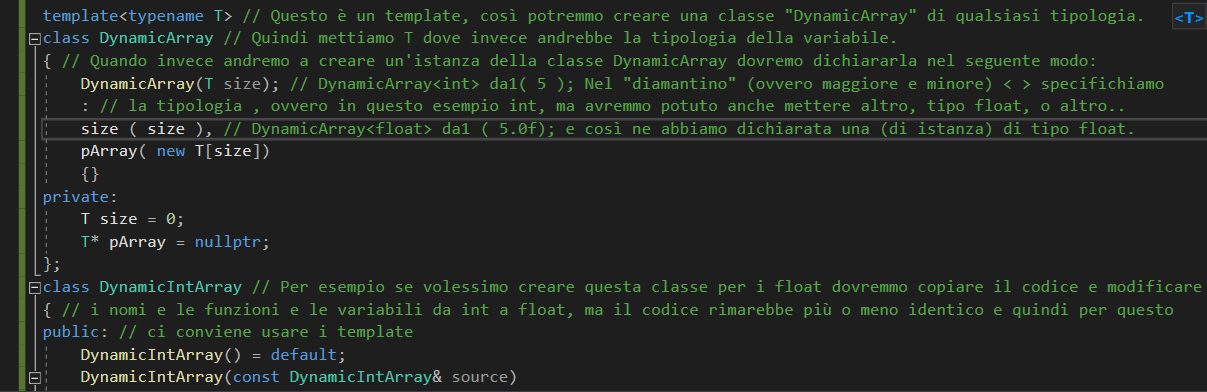
\includegraphics[width=1.2\textwidth, height=1.2\textheight, keepaspectratio]{./imgs/template.png}
	\caption{Template}
	\label{fig:template}
\end{figure}

%TODO: typename

% -------------------------- SECTION: VECTOR -----------------------------------------

%TODO: emplace_back

\section{std::vector<>}

\textsf{\small \textbf{Definizione:} I \textbf{vectors} sono un contenitore rappresentante una array che può cambiare in size (spazio). Sono degli array dinamici.} \\

\textsf{\small I vectors memorizzano i dati in locazioni contigue di memoria e permettono l'accesso diretto a qualsiasi elemento usando l'operatore []. Supportano la riduzione e l'ampiamento dello spazio a runtime (ovvero eseguite mentre il tuo programma è in esecuzione).} \\

\textsf{\small La classe vector fa uso dei template così che possiamo eseguirla con qualsiasi tipo. Per poterla usare avremo bisogno di importare \textbf{\#include <vector>}.} \\

\begin{lstlisting}
	#include <iostream>
	#include <vector>
	
	std::vector<int> v{ 1, 3, 7, 8};
	std::vector<int> v2 = v; // Oppure potevamo scrivere std::vector<int> v2(v);
	
	v2.push_back(9); // Aggiungiamo un elemento.
	
	std::cout << "v size: " << v.size() << std::endl; //Output: v size: 4
	std::cout << "v2 size: " << v2.size() << std::endl; //Output: v2 size: 5
\end{lstlisting}

\textsf{\small Inoltre, la classe vector mette a disposizione tante altre funzioni per la loro manipolazione.} \\

\textsf{\small P.S.: Da non confondere con i vettori in matematica|fisica.} \break

% -------------------------- SECTION: ITERATORI --------------------------------------

\newpage

\section{Iteratori}

\textsf{\small \textbf{Definizione: } Gli \textbf{iteratori} sono degli oggetti (come puntatori) che puntano ad un elemento all'interno di un contenitore. Usiamo gli \textbf{iteratori} per muoverci nel contenitore } \break

\textsf{\small Ci sono diversi tipi di iteratori: } \\

\begin{itemize}
	\item \textsf{\small \textbf{Input Iterators} : Sono i più deboli fra tutti per via delle loro limitate funzionalità. Può essere usato solo in algoritmi single-pass ovvero quelli che processano il contenitore in modo sequenziale.}
	\item \textsf{\small \textbf{Output Iterators} : Anch'essi sono molto limitati. Possono essere usati negli algoritmi single-pass, ma non per accedere agli elementi, ma per essere assegnati agli elementi.}
	\item \textsf{\small \textbf{Forward Iterator} : Sono più in alto nella gerarchia rispetto agli input ed output e possiedono tutte le funzionalità di questi ultimi due, ma possono anche muoversi in avanti ed anch'essi di una posizione alla volta.}
	\item \textsf{\small \textbf{Bidirectional Iterators} : Possiedono tutte le funzionalità degli forward iterators, ma possono muoversi in entrambe le direzioni.}
	\item \textsf{\small \textbf{Random-Access Iterators} : Sono gli iteratori più potenti. Non sono limitati dal solo poter muoversi in modo sequenziale, ma possono accedere in maniera casuale a qualsiasi elemento dentro ad un contenitore. Sono quelli che hanno le stesse funzionalità dei puntatori.}
\end{itemize}

\pagebreak

\begin{figure}[H]
	\centering
	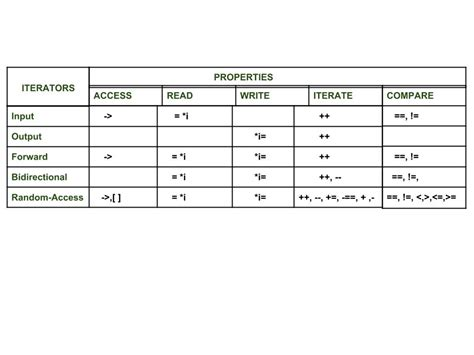
\includegraphics[width=1.2\textwidth, height=1.2\textheight, keepaspectratio]{./imgs/iterators.jpg}
	%\caption{Iteratori}
	\label{fig:iterators}
\end{figure}

\vspace{-3.69cm}

\textsf{\small È sempre meglio usare gli \textbf{iteratori} per iterare tra i contenuti di un contenitore così da evitare di usare l'operatore \textbf{[]} per accedere agli elementi. Inoltre per ottenere la fine di un contenitore con gli \textbf{iteratori} possiamo semplicemente usare la funzione \textbf{end()} al posto di utilizzare lo spazio occupato. } \break

\textsf{\small Possono essere utili per la riusabilità del codice, visto che anche se cambiamo vettore, il codice riguardante gli \textbf{iteratori} non dovrebbe cambiare.} \\

\textsf{\small Gli \textbf{iteratori} ci permettono una manipolazione dinamica dei contenitori, permettendoci di aggiungere e rimuovere elementi in modo dinamico a nostro piacimento.} \break

\textsf{\small Per poter usare gli iteratori è necessario includere \textbf{\#include <iterator>}.} \\

\begin{itemize}
	\item \textsf{\small \textbf{begin()} : Restituisce la posizione iniziale del contenitore.}
	\item \textsf{\small \textbf{end()} : Restituisce la posizione finale del contenitore.}
	%\item \textsf{\small \textbf{} :}
\end{itemize}

\begin{lstlisting}
	#include <iostream>
	#include <iterator>
	
	std::vector<int> v = { 9, 6, 3};
	
	// Dichiaro un iteratore.
	std::vector<int>::iterator it;
	for(it = v.begin(); it < v.end(); it++)
	{
		std::cout << "Elemento: " << *it << std::endl;
	}

	// Output: stampa uno ad uno gli elementi del vettore.
\end{lstlisting}

\begin{itemize}
	\item \textsf{\small \textbf{advance()} : Incrementa la posizione dell'iteratore fino all'argomento passato come parametro.}
	\item \textsf{\small \textbf{next()} : Restituisce un nuovo iteratore dopo aver avanzato di tot posizioni menzionate nell'argomento.}
	\item \textsf{\small \textbf{prev()} : Restituisce un nuovo iteratore dopo essere retrocesso di tot posizioni menzionate nell'argomento.}
	\item \textsf{\small \textbf{inserter()} : Per inserire elementi ad qualsiasi posizione nel contenitore. Prende due argomenti: il contenitore e l'iteratore alla posizione in cui l'elemento deve essere inserito.}
\end{itemize}

\begin{lstlisting}
	#include <iostream>
	#include <iterator>
	
	std::vector<int> v = { 9, 6, 3};
	std::vector<int> v2(2, 5, 8);
	
	std::vector<int>::iterator it = v.begin();
	
	std::advance(it, 2);
	
	std::cout << "Elemento dell'iteratore dopo advance: " << *it << std::endl; // Output: Elemento dell'iteratore dopo advance: 3
	
	std::prev(it, 2);
	std::cout << "Elemento dell'iteratore dopo prec: " << *it << std::endl; // Output: Elemento dell'iteratore dopo prec: 9
	
	std::next(it, 1);
	std::cout << "Elemento dell'iteratore dopo next: " << *it << std::endl; // Output: Elemento dell'iteratore dopo next: 6
	
	// Copio gli elementi di 1 vettore nell'altro usando inserter
	// Inserisco gli elementi di v2 in v alla posizione a cui puntava l'iteratore it.
	std::copy(v2.begin(), v2.end(), std::inserter(v, it));
	
	for(int &x : v)
	{
		std::cout << "Elemento: " << x << std::endl;
	}

	// Output: Gli elementi del vettore con gli elementi aggiunti.
\end{lstlisting}

%TODO: Iterable Interface?

% -------------------------- SECTION: VIRTUAL ----------------------------------------

\newpage

\section{Virtual}

\subsection{Virtual functions}

\textsf{\small \textbf{Definizione:} Una funzione \textbf{virtuale} è una funzione dichiarata in una classe base che può essere ri-definita (\emph{overridden}) da una classe derivata. Le funzioni \textbf{virtuali} ci assicurano che la corretta versione della funzione venga eseguita.} \\

\textsf{\small Alcune regole per le \textbf{funzioni virtuali}: }

\begin{itemize}
	\item \textsf{\small Non possono essere statiche.}
	\item \textsf{\small Può essere una \textbf{friend function} di un'altra classe.}
	\item \textsf{\small Bisognerebbe accedergli attraverso un puntatore o referenza di un tipo alla classe base per ottenere \emph{runtime polymorphism}.}
	\item \textsf{\small Il prototipo della funzione dovrebbe essere lo stesso sia nella classe base sia nella classe derivata.}
	\item \textsf{\small Sono sempre definiti nella classe base e ridefiniti nella classe derivata. Non è obbligatorio che la classe derivata ri-definisca la funzione, può anche soltanto utilizzare quella della classe base.}
	\item \textsf{\small Una classe può avere un \textbf{virtual destructor}, ma non un \textbf{virtual constructor}.}
\end{itemize}

\begin{lstlisting}
	#include <iostream>
	
	class Base {
		public:
			virtual void print()
			{
				std::cout << "print in base class" << std::endl;
			}
		
			void show()
			{
				std::cout << "show in base class" << std::endl;
			}
	};

	class Derived : public Base {
		public:
			void print() override // override non servirebbe, ma aiuta per la manutenzione del codice ed indica che la funzione è stata "overridata".
			{
				std::cout << "print in derived class" << std::endl;
			}
		
			void show()
			{
				std::cout << "show in derived class" << std::endl;
			}
	};

	int main()
	{
		Base* bPtr;
		Derived d;
		bPtr = &d;
		
		// Chiamo la funzione virtuale.
		bPtr->print(); // Output: print in derived class
		
		// Chiamo la funzione non virtuale.
		bPtr->show(); // Output: show in base class
		
		return 0;
	}
\end{lstlisting}

\subsection{Virtual Destructors}

\textsf{\small \textbf{Definizione:} Per rimuovere una classe derivata, la classe base dovrebbe essere definita con un \textbf{distruttore virtuale}. Cancellare una classe derivata usando un puntatore alla classe base senza un distruttore virtuale risulta in un comportamento indefinito (\emph{undefined behaviour}).} \\

\begin{lstlisting}
	#include <iostream>
	
	class A {
		public:
			A()
			{
				std::cout << "Constructor in base class" << std::endl;
			}	
		
			virtual ~A()
			{
				std::cout << "Destructor in base class" << std::endl;
			}
	};

	class B : public A {
		public:
			B()
			{
				std::cout << "Constructor in derived class" << std::endl;
			}
		
			~B()
			{
				std::cout << "Destructor in derived class" << std::endl;
			}
	};

	int main()
	{
		B* bPtr = new B();
		A* aPtr = bPtr;
		
		delete aPtr;
		
		// Output: 
		// Constructor in base class
		// Constructor in derived class
		// Destructor in derived class
		// Destructor in base class
		return 0;
	}
\end{lstlisting}

\textsf{\small In linea di massima, se si ha una funzione virtuale, allora è da mettere anche il distruttore virtuale.} \break

\subsection{Virtual Inheritance}

\textsf{\small \textbf{Definizione:} La \textbf{Ereditarietà virtuale} è usata per risolvere il problema del \textbf{DDD} (\emph{Dreadful Diamond on Derivation}), ovvero quando una classe deriva molteplici classi che derivano dalla stessa classe.} \\

\begin{figure}[H]
	\centering
	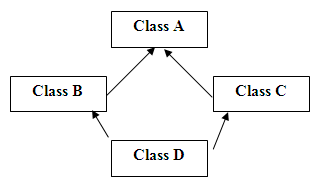
\includegraphics[width=1\textwidth, height=1\textheight, keepaspectratio]{./imgs/diamond_problem2.png}
	\caption{Problema del diamante}
	\label{fig:diamond_problem}
\end{figure}

\textsf{\small Come possiamo notare i dati e le funzioni della \textbf{classe A} è ereditata due volte dalla \textbf{classe D}, una volta per via della \textbf{classe B} e una volta per via della \textbf{classe C}.} \\

\textsf{\small Quando qualsiasi dato o funzione della \textbf{classe A} viene acceduto dalla \textbf{classe D}, nasce dell'ambiguità su quale dato/funzione chiamare. Quella ereditata da \textbf{B} o da \textbf{C}? Questo confonde i compilatori e mostrano errori.}

\textsf{\small Per risolvere questa ambiguità quando la \textbf{classe A} è ereditata sia dalla \textbf{classe B} sia dalla \textbf{classe C}, è dichiarata come \textbf{classe base virtuale} (Fare riferimento all'immagine: \textbf{\ref{fig:diamond_problem}} a \textbf{pag.\pageref{fig:diamond_problem}}).}

\begin{lstlisting}
	#include <iostream>
	
	class A {
		public:
			void show()
			{
				std::cout << "Show from A" << std::endl;
			}
	};

	class B : public virtual A {
	};

	class C : public virtual A {
	};

	class D : public B, public C {
	};

	int main()
	{
		D d;
		d.show(); // Output: Show from A
	}
\end{lstlisting}

\textsf{\small La keyword \textbf{virtual} può essere posta sia prima che dopo \textbf{public}.} \\

%TODO: Aggiungere immagini: "virtual_functions_recap_terminology_and_concepts".
%TODO: Aggiungere immagini: "virtual_functions_implementation".

% -------------------------- SECTION: POLYMORPHISM -----------------------------------

\section{Polimorfismo}

\textsf{\small \textbf{Definizione:} La parola \textbf{polimorfismo} significa \emph{avere molte forme}, questo occorre quando c'è una gerarchia di classi e queste sono correlate attraverso l'ereditarietà.} \\

\textsf{\small Ci sono due tipi principali di polimorfismo: }

\begin{itemize}
	\item \textsf{\small \textbf{Compile time Polymorphism} : si ottiene dall'\emph{overloading} di funzioni o di operatori.}
	\item \textsf{\small \textbf{Runtime Polymorphism} : si ottiene dall' \emph{overriding} delle funzioni (con la keyword \textbf{virtual}).}
\end{itemize}

\begin{figure}[H]
	\centering
	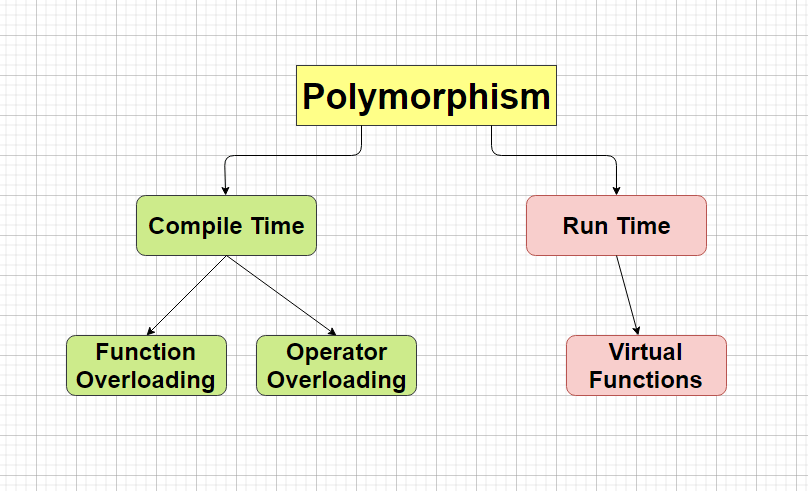
\includegraphics[width=1\textwidth, height=1\textheight, keepaspectratio]{./imgs/polymorphism.png}
	\caption{Polimorfismo}
	\label{fig:polymorphism}
\end{figure}

% -------------------------- SECTION: OVERLOADING ------------------------------------

\section{Overloading}

\textsf{\small \textbf{Definizione:} L'\textbf{overloading} permette di ridefinire una funzione o un operatore con lo stesso nome e nello stesso scope, ma con una differente implementazione.} \\

\subsection{Function Overloading}

\textsf{\small Si può definire una funzione con lo stesso nome di un'altra purchè abbia argomenti diversi.} \\

\begin{lstlisting}
	void func(int x)
	{
		std::cout << "Valore di x: " << x << std::endl;
	}

	void func(double x)
	{
		std::cout << "Valore di x: " << x << std::endl;
	}

	void func(float x)
	{
		std::cout << "Valore di x: " << x << std::endl;
	}
\end{lstlisting}

\subsection{Operator Overloading}

\textsf{\small Possiamo ridefinire degli operatori per eseguire delle operazioni nel modo che vogliamo noi.} \\

\textsf{\small Utilizziamo la keyword \textbf{operator} ed il simbolo dell'operatore per \emph{overloaddarlo}.} \\

\begin{lstlisting}
	class Vec {
		public:
			Vec(){}
		
			Vec(int x, int y)
			{
				this->x = x;
				this->y = y;
			}
		
			Vector operator+(const Vec& v)
			{
				Vec vec;
				vec.x = this->x + v.x;
				vec.y = this->y + v.y;
				return vec;
			}
		
			int getX()
			{
				return this->x;
			}
		
			int getY()
			{
				return this->y;
			}
		
		private:
			int x;
			int y;
	};

	int main()
	{
		Vec v1(3, 2);
		Vec v2(1, 0);
		
		Vec v3 = v1 + v2;
		
		std::cout << "v3.x: " << v3.getX() << "; v3.getY(): " << v3.y << std::endl;
		// Output: v3.x: 4; v3.y: 2
		// perché facciamo la x di v1 che è 3 + la x di v2 che è 1 quindi 4 e 
		// la y di v1, ovvero 2 + la y di v2, ovvero 0 quindi 2
		// quindi v3 ha membri (4,2).
		return 0;
	}
\end{lstlisting}

\textsf{\small Non tutti gli operatori si possono \emph{overloaddare}.} \\

\textsf{\small Gli operatori che non si possono \emph{overloaddare} sono: \textbf{.} (punto), \textbf{::}, \textbf{?:}(operatore ternario), \textbf{sizeof}.} \\

\subsection{Overloading vs Overriding}

\textsf{\small L'\textbf{overloading} è la creazione di molteplici definizioni di una funzione cambiando la \textbf{signature}: il numero di parametri, la tipologia dei parametri. Il tipo di ritorno non gioca alcun ruolo.} \\

\textsf{\small Può essere fatta sia nelle classi basi che in quelle derivate.} \break

\textsf{\small L'\textbf{overriding} è la ridefinizione di una funzione di una classe base in una classe derivata con la stessa \textbf{signature}, stesso tipo di ritorno e parametri.} \\

\textsf{\small Può essere fatta solo nelle classi derivate.} \break

\textsf{\small Differenza tra \textbf{function overloading} e \textbf{function overriding}: } \break

\begin{tabular}{|c|c|} %TODO: questo è da riguardare, perché la fonte forse ha fatto degli errori.
	\hline
	\textbf{Overloading} & \textbf{Overriding} \\
	\hline
	\textsf{\small Nessuna keyword è usata.} & \textsf{\small Keyword \textbf{override}.} \\
	\hline
	\textsf{\small Il prototipo cambia } & \textsf{\small Il prototipo non cambia.} \\
	\textsf{\small in base ai parametri.} & \textsf{\small } \\
	\hline
	\textsf{\small Occorre durante compile time.} & \textsf{\small Occorre durante runtime.} \\
	\hline
	\textsf{\small I costruttori possono } & \textsf{\small } \\
	\textsf{\small essere "overloaddati".} & \textsf{\small } \\
	\hline
	\textsf{\small I distruttori non } & \textsf{\small I distruttori } \\
	\textsf{\small possono essere "overloaddati".} & \textsf{\small possono essere "overridati".} \\
	\hline
	\textsf{\small } & \textsf{\small Le funzioni virtuali } \\
	\textsf{\small } & \textsf{\small non possono essere "overridate".} \\
	\hline
	\textsf{\small Può essere usato per ottenere } & \textsf{\small Overriding è anche conosciuto come } \\
	\textsf{\small \emph{early binding}.} & \textsf{\small \emph{late binding}.} \\
	\hline
	\textsf{\small La funzione chiamata viene } & \textsf{\small La funzione overriden} \\
	\textsf{\small determinata dal numero} & \textsf{\small è preceduta} \\
	\textsf{\small di parametri.} & \textsf{\small dalla keyword virtual nella classe base.} \\
	\hline
	\textsf{\small Le funzioni verrebbero} & \textsf{\small } \\
	\textsf{\small ridefinite} & \textsf{\small } \\
	\textsf{\small con lo stesso nome, ma} & \textsf{\small } \\
	\textsf{\small differente numero o tipo} & \textsf{\small } \\
	\textsf{\small di parametri.} & \textsf{\small } \\
	\hline
	\textsf{\small } & \textsf{\small L'indirizzo dell'oggetto} \\
	\textsf{\small } & \textsf{\small della classe è assegnato al} \\
	\textsf{\small } & \textsf{\small puntatore la cui funzione} \\
	\textsf{\small } & \textsf{\small è chiamata dal puntatore.} \\
	\hline
	\textsf{\small } & \textsf{\small Quando la funzione è definita viene preceduta} \\
	\textsf{\small } & \textsf{\small dalla keyword virtual nel main.} \\
	%\textsf{\small } & \textsf{\small La stessa funzione è ridefinita } \\
	%\textsf{\small } & \textsf{\small nella classe derivata usando} \\
	%\textsf{\small } & \textsf{\small la keyword \textbf{out}.} \\
	%\textsf{\small } & \textsf{\small } \\
	\hline
\end{tabular}

% -------------------------- SECTION: TIPI DI CAST -----------------------------------

\newpage

\section{Tipi di Casts}

\textsf{\small \textbf{Definizione:} Il \textbf{casting} è un'operazione che permette la conversione di un valore in un altro. In C++ ci sono diversi tipi di casting: } \\

\subsection{static\_cast<>}

\begin{itemize}
	\item \textsf{\small \textbf{static\_cast<> :} Quello che fa è un cast implicito tra tipi (come int a float, o puntatore a void*) e può anche chiamare funzioni esplicite per la conversione. }
\end{itemize}

\begin{lstlisting}
	float f = 3.69;
	int x = static_cast<int>(f);
	std::cout << "x: " << x << std::endl; // Output: x: 3 
\end{lstlisting}

\subsection{const\_cast<>}

\begin{itemize}
	\item \textsf{\small \textbf{const\_cast<> :} Serve per aggiungere o rimuovere il \textbf{const} ad una variabile. Se la variabile che stiamo cercando di modificare era già const allora questo produce un valore indefinito. Se lo si usa per qualcosa che non era dichiarato come const allora è safe (sicuro farlo, non ci saranno problemi).  }
\end{itemize}

\begin{lstlisting}
	#include <iostream>
	
	void print( char* str)
	{
		std::cout << str << '\n';
	}

	int main()
	{
		const char* c = "testo";
		// Ci serve per poter passare un puntatore a char const ad una funzione che prende un puntatore a char senza const.
		print(const_cast<char*>(c)); // Output: testo
		return 0;
	}
\end{lstlisting}

\subsection{dynamic\_cast<>}

\begin{itemize}
	\item \textsf{\small \textbf{dynamic\_cast<> :} Serve esclusivamente per i casts riguardanti il polimorfismo. Puoi castare un puntatore o una reference a qualsiasi altro tipo di classe. Non solo si può fare un casting verso il basso, ma anche in alto e a lato. Il dynamic\_cast cercherà di ritorna l'oggetto desiderato se possibile, altrimenti ritornerà \textbf{nullptr} in caso di un puntatore e \textbf{std::bad\_cast} nel caso di una reference.}
	\item \textsf{\small Ha delle limitazioni. Non funzionerà nel caso in cui diversi oggetti ereditano tutti dallo stessa classe. (il famoso problema del \emph{dreaded diamond}.) e non stai usando l'ereditarietà \textbf{virtual}.}
	\item \textsf{\small Inoltre può soltanto funzionare con l'ereditarietà pubblica, fallirà con l'ereditarietà \textbf{protected} o \textbf{private}. Comunque questi tipi di ereditarietà sono rare.}
\end{itemize}

\begin{lstlisting}
	// C++ programma per dimostrare che se non c'è
	// alcuna funzione virtuale nella Base classe.
	#include <iostream>
	
	// Base class declaration
	class Base {
		void print()
		{
			std::cout << "Base" << std::endl;
		}
	};
	
	// Derived Class 1 declaration
	class Derived1 : public Base {
		void print()
		{
			std::cout << "Derived1" << std::endl;
		}
	};
	
	// Derived class 2 declaration
	class Derived2 : public Base {
		void print()
		{
			std::cout << "Derived2" << std::endl;
		}
	};
	
	// Driver Code
	int main()
	{
		Derived1 d1;
		
		// Base class pointer hold Derived1
		// class object
		Base* bp = dynamic_cast<Base*>(&d1);
		
		// Dynamic casting
		Derived2* dp2 = dynamic_cast<Derived2*>(bp);
		if (dp2 == nullptr)
			std::cout << "null" << std::endl;
			
		// Output: null, in realtà errore.
		return 0;
	}
\end{lstlisting}

\subsection{reinterpret\_cast<>}

\begin{itemize}
	\item \textsf{\small \textbf{reinterpret\_cast<> :} È quello più pericoloso di tutti e quindi bisogna utilizzarlo con moderazione. Trasforma un tipo direttamente in un altro come cast da un puntatore ad un altro o memorizzare un puntatore in un int, ecc..}
	\item \textsf{\small L'unica cosa garantita con questo tipo di cast è che se torni indietro al tipo originale riotterrai lo stesso valore (non succederà se il tipo era più piccolo del tipo originale.)}
\end{itemize}

\begin{lstlisting}
	class A {
		public:
			int x;
	};

	class B {
		public:
			int x;
	};

	A *a = new A;
	B *b = reinterpret_cast<*B>(a);
	
	a->x = 5;
	std::cout << "b: " << b->x << std::endl; // Output: b: 5
	std::cout << "a: " << a->x << std::endl; // Output: a: 5
\end{lstlisting}

\subsection{C-style \& function-style cast o Regular Cast}

\begin{itemize}
	\item \textsf{\small Questo tipo di cast chiamato \textbf{Regular Cast} o \textbf{C-style cast} (derivando dal C ovviamente) è molto più potente degli altri tipi di cast, ma allo stesso tempo molto meno sicuro.}
	\item \textsf{\small Ignorano i controlli d'accesso quando si esegue uno static\_cast.}
	\item \textsf{\small Permette di fare un cast sicuro ad una classe privata, mentre il suo "equivalente" static\_cast darebbe un errore a tempo di compilazione (compile-time).}
\end{itemize}

\begin{lstlisting}
	double d = 9.87;
	int x;
	
	x = (int)d;
	std::cout << "x: " << x std::endl; // Output: x: 9
\end{lstlisting}

\subsection{Ricapitolando}

\begin{tabular}{|c|c|}
	\hline
	\textbf{Cast} & \textbf{Definizione} \\
	\hline
	\textbf{dynamic\_cast} & \textsf{\small per convertire puntatori/references in una gerarchia di ereditarietà.} \\
	\hline
	\textbf{static\_cast} & \textsf{\small per le conversioni di tipi ordinari.} \\
	\hline
	\textbf{reinterpret\_cast} & \textsf{\small per reinterpretare bit patterns di basso livello. Usare con cauzione.} \\
	\hline
	\textbf{const\_cast} & \textsf{\small per aggiungere/rimuovere \textbf{const} al cast.} \\
	\hline
\end{tabular}

\begin{figure}[ht]
	\centering
	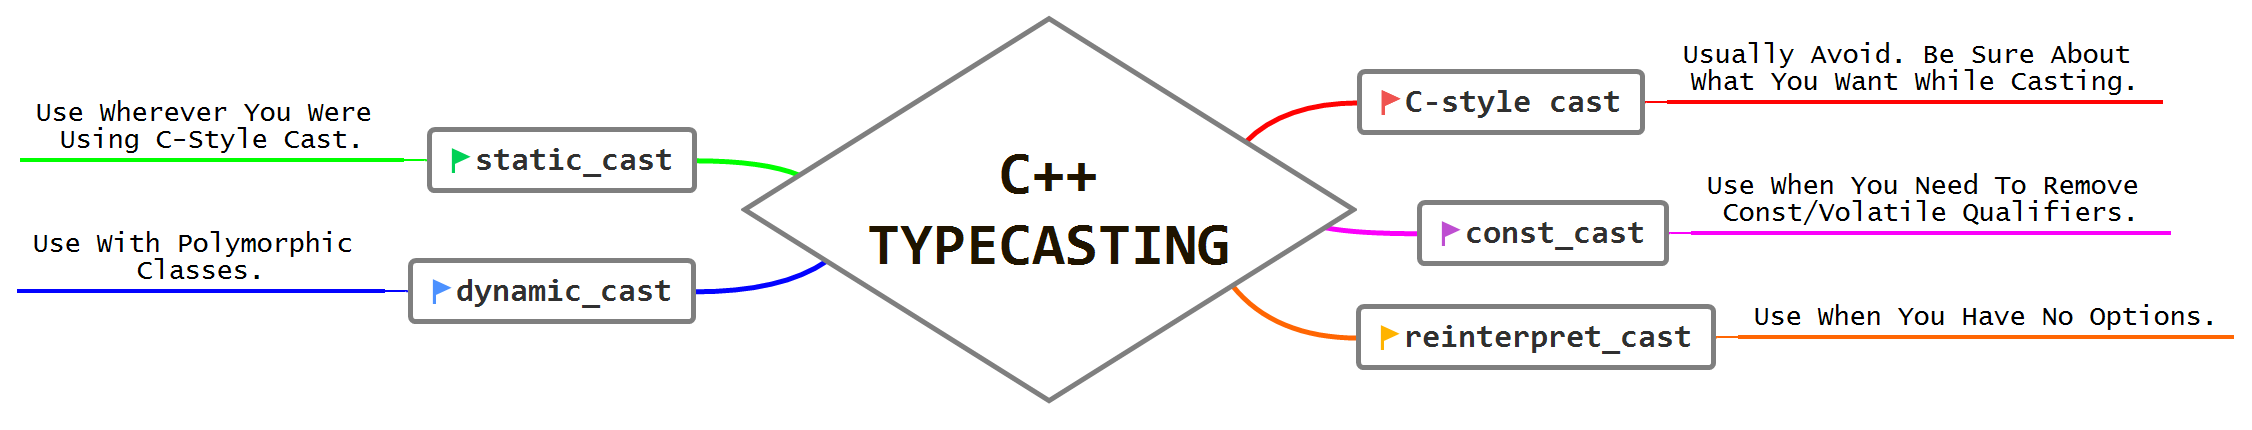
\includegraphics[width=1.2\textwidth, height=1.2\textheight, keepaspectratio]{./imgs/typecasting.png}
	\caption{Typecasting}
	\label{fig:typecasting}
\end{figure}

%TODO: Aggiungere immagine "cast_types_recap_static_dynamic_reinterpret_const_c-style".

%TODO: typeid

% -------------------------- SECTION: LAMBDAS ----------------------------------------

%TODO: potrei mettere le lambbdas subito dopo gli iteratori.

\section{Lambdas}

\textsf{\small \textbf{Definizione:} Dal C++11 sono presenti le \textbf{lambdas} che permettono di creare \textbf{funzioni anonime}.} \\

\textsf{\small Servono per creare delle funzioni, dei piccoli frammenti di codice che non hanno bisogno di un nome e non verranno riutilizzati. } \\ % funzioni inline

\textsf{\small Sono una parte centrale della \textbf{programmazione funzionale}.} \\

\textsf{\small Questa è la struttura di una tipica espressione \textbf{lambda} :} \\

\begin{lstlisting}
	[ clausola di cattura ] ( lista di parametri che è opzionale) -> tipoDiRitorno
	{
		// Definizione della lambda.
	}
\end{lstlisting}

\textsf{\small Se nella clausola della cattura è presente un \textbf{=} (uguale), vuol dire che la lambda può accedere a qualsiasi variabile, se c'è un \textbf{\&} vuol dire che stiamo accedendo alle variabili per reference, se la clausola [] è vuota allora può accedere soltanto alle variabili locali, altrimenti lì saranno presenti i nomi delle variabili che si vogliono utilizzare ("catturate" o per valore o per reference).} \\ %TODO: forse si potrebbe rimuovere questa parte e lasciare solo la tabella.

\begin{tabular}{|c|c|}
	\hline
	\textbf{Cattura} & \textbf{Definizione} \\
	\hline
	\textsf{\small []} & \textsf{\small accedere solo alla variabili locali} \\
	\hline
	\textsf{\small [=]} & \textsf{\small accedere a tutte le variabili per valore.} \\
	\hline
	\textsf{\small [\&]} & \textsf{\small accedere a tutte le variabili per reference.} \\
	\hline
	\textsf{\small [nomeVariabile1, \&nomeVariabile2]} & \textsf{\small "cattura" nomeVariabile per valore } \\
	\textsf{\small } & \textsf{\small e nomeVariabile2 per referenza.} \\
	\hline
\end{tabular} \\

\begin{lstlisting}
	#include <iostream>
	#include <vector>
	
	std::vector<int> v1 = { 5, 8, 9, 1, 7};
	std::vector<int> v2 = {12, 36, 27, 92};
	
	// Lambda.
	auto pushinto = [&](int m)
	{
		v1.push_back(m);
		v2.push_back(m);
	}; // Da notare il ; alla fine.

	// Pusha in entrambi v1 e v2 il numero 24
	pushinto(24);
	
	// Lambda, accediamo a v1 per valore (quindi ne facciamo una copia).
	[v1]()
	{
		for(auto p = v1.begin(); p != v1.end(); p++)
		{
			std::cout << *p << std::endl;
		}
	};

	int n = 7;
	// trova il primo numero maggiore di n.
	// [n] significa che stiamo accedendo e possiamo soltanto accedere ad n (per valore, ovvero una copia di essa).
	std::vector<int>:: iterator p = std::find_if(v1.begin(), v1.end(), [n](int i)
	{
		return i > n;
	});

	std::cout << "Il primo numero maggiore di n e\': " << *p << std::endl; // Output: Il primo numero maggiore di n e\': 8

	// Qui [=] vuol dire che possiamo accedere a tutte le variabili.
	int countN = std::count_if(v1.begin(), v1.end(), [=](int a) 
	{
		return a >= n;
	});

	std::cout << "Il numero di elementi piu' grandi o uguali ad n sono: " << countN << std::endl; // Output: Il numero di elementi più grandi o uguali ad n sono: 4 (perchè abbiamo inserito anche il 24 nell'operazione precedente).
\end{lstlisting}

%TODO: capture.
%TODO: poi trattare anche dei functors.

% -------------------------- SECTION: MEMORIA DINAMICA -------------------------------

\newpage

\section{Memoria dinamica}

\textsf{\small \textbf{Definizione: } Riguarda l'allocazione di memoria manualmente da parte del programmatore. La memoria allocata dinamicamente è allocata nell' \textbf{Heap} mentre le variabili locali e la memoria non statica viene allocata nello \textbf{Stack}.}

\begin{itemize}
	\item \textsf{\small \textbf{Heap} : memoria dinamica.}
	\item \textsf{\small \textbf{Stack} : variabili locali e non-statiche.}
\end{itemize}

\subsection{Memoria Dinamica in C}

\textsf{\small In C per l'allocazione dinamica della memoria usufruivamo di 4 diverse funzioni: \textbf{malloc()} (per allocare), \textbf{calloc()}, \textbf{realloc()} (per riallocare), \textbf{free()} (per liberare la memoria).} \\

\textsf{\small Tutte questi funzioni del C, esistono anche nel C++, ma questo ha un suo modo per l'allocazione dinamica della memoria.} \break

\subsection{new e delete}

\subsubsection{new}

\textsf{\small \textbf{Definizione: } L'operatore \textbf{new} denota una richiesta di allocazione di memoria nello spazio libero. Se sufficiente memoria è disponibile, l'operatore inizializza la memoria e restituisce l'indirizzo della nuova memoria allocata ed inizializzata al puntatore.} \\

\begin{lstlisting}
	// Esempio 1
	int *ptr = nullptr;
	ptr = new int;
	
	// Esempio 2
	double *dPtr = new double;
	
	// Esempio 3
	int *p = new int(22);
	
	// Esempio 4
	int *pArray = new int[12];
\end{lstlisting}

\subsubsection{array normali vs array con la new}

\textsf{\small L'unica differenza è che gli array normali vengono deallocati dal compilatore, mentre quelli creati con la new devono essere deallocati dal programmatore.} \break

\subsubsection{delete}

\textsf{\small \textbf{Definizione: } Utilizziamo la keyword \textbf{delete} per deallocare la memoria precedentemente allocata.} \\

\begin{lstlisting}
	// Esempio 1
	int *ptr = new int;
	
	delele ptr;
	
	// Esempio 2
	int *p = new int[6];
	
	delete[] p;
\end{lstlisting}

\subsection{Evitare di usare new}

\textsf{\small \textbf{Definizione: } Ci sono vari motivi per cui evitare o minimizzare gli utilizzi della keyword \textbf{new}: } \\

\begin{itemize}
	\item \textsf{\small Il C++ non ha un garbage collector, quindi per ogni \textbf{new} ci deve essere una corrispondente \textbf{delete}.}
	\item \textsf{\small Se viene lanciata un'eccezione poi la memoria non viene mai liberata.}
	\item \textsf{\small Dovrebbe essere tutto nel distruttore, concetto del \emph{RAII}.} %TODO: add ref quando ne parlerò.
	\item \textsf{\small Se restituisci per esempio una stringa a qualcuno, ora sono loro a doverla cancellare (con la \textbf{delete}). E se a loro volta la passassero come argomento? Quando dovrebbe essere liberata? (con \textbf{delete}).}
	\item \textsf{\small Può essere un problema nel multi-threading.}
	\item \textsf{\small Potrebbe portare a dei \emph{memory leaks}.}
\end{itemize}

% -------------------------- SECTION: RAII -------------------------------------------

\section{RAII | Resource Acquisition is initialization}

\textsf{\small \textbf{Definizione: } \textbf{RAII} (\emph{Resource Acquisition is Initialization}) è un idioma comune della programmazione e della gestione delle risorse. Ogni allocazione della risorsa è fatta alla creazione dell'oggetto da parte del \textbf{costruttore} mentre la deallocazione (rilascio della memoria) viene fatto dal \textbf{distruttore}. Quindi se non ci sono leaks all'oggetto, non ci sono leaks nemmeno alla risorse. } \\

\begin{figure}[ht]
	\centering
	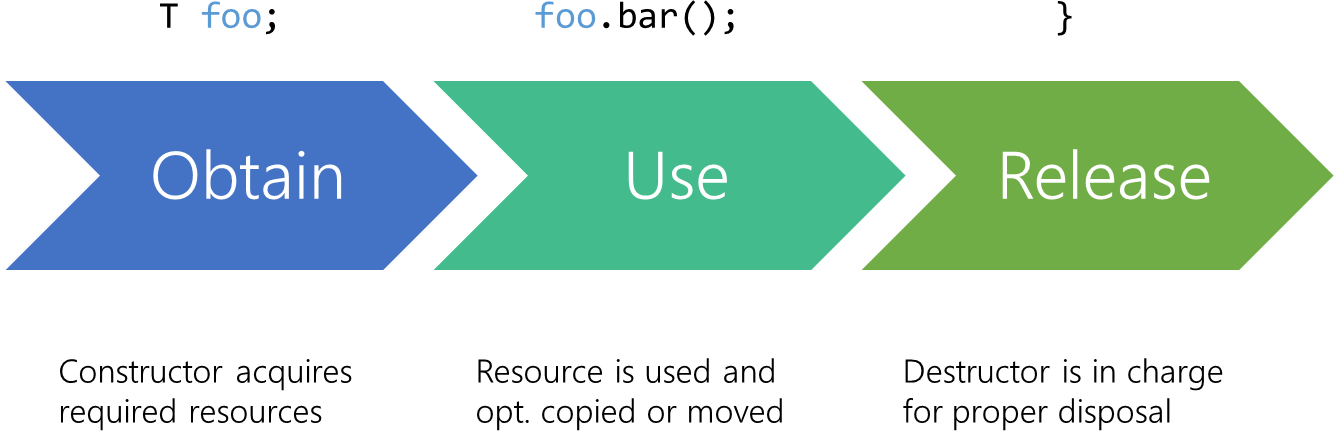
\includegraphics[width=1\textwidth, height=1\textheight, keepaspectratio]{./imgs/RAII.png}
	\caption{RAII}
	\label{fig:RAII}
\end{figure}

%TOOD: magari approfondire l'argomento.

% -------------------------- SECTION: TIPI DI COSTRUTTORI | RULE OF 3 ----------------

\section{Constructor types | Rules of}

%TODO: explicit constructor, converting constructor.
%TODO: Private Destructor

\subsection{Rule of Zero}

\textsf{\small \textbf{Definizione: } La \textbf{regola dello zero} (è una regola generale/un'indicazione) afferma che se non hai bisogno di nessuno di questi, allora non ne devi implementare nessuno: } \\

\begin{itemize}
	\item \textsf{\small \textbf{Distruttore} : libera tutte le risorse precedentemente allocate.}
	\item \textsf{\small \textbf{Copy Constructor} : Fa una copia di un oggetto.}
	\item \textsf{\small \textbf{Copy assign} : overload dell'operatore di assegnamento.}
\end{itemize}

\subsection{Copy Constructor}

\textsf{\small \textbf{Definizione: } Il \textbf{Copy Constructor} è un tipo di costruttore che inizializza un oggetto usando un altro oggetto della stessa classe.} \\

\textsf{\small Un costruttore di copia ha la seguente struttura: } \\

\begin{lstlisting}
	// È un costruttore quindi si chiama con il nome della classe.
	NomeDellaClasse(const NomeDellaClasse &vecchioOggetto);
\end{lstlisting}

\textsf{\small Un copy constructor potrebbe essere chiamato per:}

\begin{enumerate}
	\item \textsf{\small Quando un oggetto della classe è ritornato per valore.}
	\item \textsf{\small Quando un oggetto della classe è passato come argomento ad una funzione per valore.}
	\item \textsf{\small Quando un oggetto è costruito sulla base di un altro oggetto.}
	\item \textsf{\small Quando il compilatore genera un oggetto temporaneo.}
	%\item \textsf{\small }
\end{enumerate}

\begin{lstlisting}
	class Point {
		public:
			// Costruttore normale
			Point(int x, int y)
			{
				this->x = x;
				this->y = y;
			}
			
			// Copy Constructor
			// Assiegnamo i valori di x ed y in base ai valori di un'istanza p della classe Point.
			Point(const Point &p)
			{
				this->x = p.x;
				this->y = p.y;
			}
		
			int getX() { return this->x };
			int getY() { return this->y };
		
		private:
			int x;
			int y;
	};

	int main()
	{
		Point p1(3, 5); // Il costruttore normale viene chiamato qui.
		Point p2 = p1; // Il Copy Constructor viene chiamato qui.
		
		std::cout << "p1.x: " << p1.getX() << ", p1.y: " << p1.getY() << "\n"; // Output: p1.x: 3, p1.y: 5
		std::cout << "p2.x: " << p2.getX() << ", p2.y: " << p2.getY() << "\n"; // Output: p2.x: 3, p2.y: 5
		
		return 0;
	}
\end{lstlisting}

\subsection{Copy Assign}

\textsf{\small \textbf{Definizione: } Il \textbf{copy assignment operator} è ciò che ti permette di assegnare, di copiare un'istanza e di portare i suoi dati in un' altra istanza.} \\

\textsf{\small È usato per rimpiazzare i dati di un oggetto precedentemente inizializzato con i dati di qualche altro oggetto.} \\

\textsf{\small Se non si dichiara un \textbf{assignment operator} allora il compilatore provvederà a fornirtene uno automaticamente.} \\

\textsf{\small In linea di massima, se hai bisogno di un \textbf{copy constructor} allora avrai bisogno anche di un \textbf{copy assignment operator}.} \\

%TODO: da riguardarsi il copy assignment operator nel codice.
\begin{lstlisting}
	class Point {
		public:
			// Normal Constructor
			Point(int x, int y)
			{
				this->x = x;
				this->y = y;
			}
		
			// Copy Constructor
			Point(const Point& p)
			{
				this->x = p.x;
				this->y = p.y;
			}
		
			// Copy Assignment
			Point& operator=(const Point& p)
			{
				this->x = p.x;
				this->y = p.y;
				return *this;
			}
			
			int getX() { return this->x };
			int getY() { return this->y };
			
		private:
			int x;
			int y;
	};
\end{lstlisting}

%TODO: copy constructor = delete, copy assignment = delete.

\subsection{=default | Defaulted Functions}

\textsf{\small \textbf{Definizione: } Le \textbf{defaulted functions} in modo esplicito permette di aggiungere \textbf{=default} alla fine di una funzione per dichiararla una \emph{funzione default esplicita}. Questi sono più efficienti.} \\

\begin{lstlisting}
	class A {
		public:
		A(int a)
		{
			this->a = a;
			this->b = 0;
		}
	
		A(int a, int b) = default
		{
			this->a = a;
			this->b = b;
		};
	
		// Non ci sarebbe bisogno di mettere =default al costruttore A(), perché questo è già il costruttore di default.
		A(); 
		
		int a;
	};

	int main()
	{
		// Eseguito usando il default constructor
		A a(2);
		
		// Eseguito usando il costruttore parametrizzato.
		A b(5, 7);
		return 0;
	}
\end{lstlisting}

\subsection{=delete | Deleted Functions}

\textsf{\small \textbf{Definizione: } Apparte, deallocare la memoria, dal C++11 la \textbf{delete} ha un nuovo significato: \emph{disabilitare l'utilizzo di una funzione membra}. Queste funzioni sono conosciute come \textbf{funzioni deleted esplicitamente}.} \\

\begin{lstlisting}
	class A {
		public:
			A(int a): x(a)
			{
				this->a = a;
			}
		
			// Disabilitare il copy constructor.
			A(const A& ) = delete;
			
			// Disabilitare il copy assignment operator.
			A& operator=(const A& ) = delete;
			
			int x;
	};

	int main()
	{
		A a1(3), a2(6), a3(9);
		
		// Errore, l'utilizzo del copy assignment operator è disabilitato.
		a1 = a2;
		
		// Errore, l'utilizzo del copy constructor è disabilitato.
		a3 = A(a2);
		return 0;
	}
\end{lstlisting}

\textsf{\small \textbf{Ma qual è l'utilità di far ciò?}} \\

\begin{enumerate}
	\item \textsf{\small Previene il compilatore dal generare le \textbf{special member functions} (costruttori, distruttori, copy constructor, ecc..) che non vogliamo.} \\
	\item \textsf{\small Il disabilitare le normali funzioni membro o non-membro previene problemi di promozioni di tipo dal causare una chiamata involontaria alla funzione.} \\
	%\item \textsf{\small } \\
\end{enumerate}

\subsection{Copy Constructor vs Copy Assignment Operator}

\begin{tabular}{|c|c|}
	\hline
	\textbf{Copy Constructor} & \textbf{Copy Assignment Operator} \\
	\hline
	\textsf{\small È chiamato quando una } & \textsf{\small È chiamato quando ad un oggetto } \\
	\textsf{\small nuova istanza viene creata da } & \textsf{\small già inizializzato gli viene } \\
	\textsf{\small un oggetto già esistente, } & \textsf{\small assegnato un nuovo valore } \\
	\textsf{\small come copia di questo.} & \textsf{\small da un oggetto già esistente.} \\
	\hline
	\textsf{\small Crea un nuovo blocco di memoria} & \textsf{\small Non crea un nuovo blocco di memoria.} \\
	\textsf{\small per il nuovo oggetto.} & \textsf{\small } \\
	\hline
	\textsf{\small È un costruttore overloaded.} & \textsf{\small È un operatore bitwise.} \\
	\hline
	\textsf{\small Il compilatore fornisce} & \textsf{\small Una copia bitwise viene creata} \\
	\textsf{\small implicitamente un copy constructor} & \textsf{\small se l'assignment operator} \\
	\textsf{\small se uno non ne esiste già.} & \textsf{\small non viene overloaded.} \\
	%\textsf{\small } & \textsf{\small } \\
	\hline
\end{tabular}

\subsection{Rule of Three}

\textsf{\small \textbf{Definizione: } La \textbf{regola dei tre}, essenzialmente, afferma che se uno (o anche più) tra questi è definito, allora tutti e tre dovrebbero essere definiti: } \\

\begin{itemize}
	\item \textsf{\small \textbf{Distruttore} : libera tutte le risorse precedentemente allocate.}
	\item \textsf{\small \textbf{Copy Constructor} : Fa una copia di un oggetto.}
	\item \textsf{\small \textbf{Copy assignment operator} : overload dell'operatore di assegnamento.}
\end{itemize}

\textsf{\small I costruttori e gli assignment operator generati implicitamente fanno una \textbf{shallow copy} (copia dei dati di tutte le variabili dell'oggetto originale. Ha problemi se i dati son allocati con memoria dinamica, in quel caso faranno referenza alla stessa locazione di memoria) dei dati membri. Noi abbiamo bisogno di una \textbf{deep copy} (copia dei dati di tutte le variabili e alloca simili risorse di memoria con lo stesso oggetto) quando la classe contiene puntatori che puntano a risorse di memoria allocate dinamicamente.} \\

\subsection{Move Constructor}

\textsf{\small \textbf{Definizione: } I \textbf{Move Constructor} lavorano con le referenze \textbf{rvalue} e le \textbf{move semantics}(le move semantics riguardano il puntare ad un oggetto già esistente in memoria). Fa puntare il puntatore del nuovo oggetto ai dati dell'oggetto temporaneo e pone a null il puntatore degli oggetti temporanei.} \\

\textsf{\small I \textbf{Move Constructors} spostano le risorse nell'\emph{heap} e l'assegnano al nuovo oggetto. A differenza dei \textbf{copy constructors} i \textbf{move constructors} prevengono dall'inutile copiatura di dati di memoria.} \\

\begin{lstlisting}
	#include <iostream>
	#include <vector>
	
	class A {
		public:
			// Costruttore
			A(int x)
			{
				data = new int;
				*data = x;
				std::cout << "Costruttore chiamato per " << x << std::endl;
			}
		
			// Copy Constructor
			A(const A& source) 
			: A { *source.data }
			{
				std::cout << "Copy constructor in deep copy chiamato per " << *source.data << std::endl;
			}
		
			// Move Constructor
			A(A&& source) : data {source.data}
			{
				std::cout << "Move Constructor chiamato per " << *source.data << std::endl;
				source.data = nullptr;
			}
		
			// Distruttore
			~A()
			{
				if( data != nullptr)
				{
					std::cout << "Distruttore chiamato per " << *data << std::endl;
				} else {
					std::cout << "Distruttore chiamato per nullptr " << std::endl;
				}
				
				// Liberiamo la memoria assegnata all'oggetto.
				delete data;
			}
	};

	int main()
	{
		// Vector della classe A.
		std::vector<A> vec;
		
		// Inseriamo oggetti della classe A.
		vec.push_back(A {9} );
		vec.push_back(A {18} );
		
		// Output:
		// Costruttore chiamato per 9
		// Move Constructor chiamato per 9
		// Distruttore chiamato per nullptr 
		// Costruttore chiamato per 18
		// Move Constructor chiamato per 18
		// Costruttore chiamato per 9
		// Copy constructor in deep copy chiamato per 9
		// Distruttore chiamato per 9
		// Distruttore chiamato per nullptr 
		// Distruttore chiamato per 9
		// Distruttore chiamato per 18
		
		return 0;
	}
\end{lstlisting}

\subsubsection{lvalues references \& rvalues references}

\textsf{\small \textbf{Definizione: } Gli \textbf{l-values} fanno riferimento alla locazione di memoria che definisce l'oggetto. Gli \textbf{r-values} fanno riferimento al valore che è memorizzato in qualche indirizzo di memoria.} \\

\textsf{\small Proprietà degli \textbf{r-values}:} \\

\begin{itemize}
	\item \textsf{\small Estendono la durata di vita degli oggetti temporanei a cui sono assegnati.}
	\item \textsf{\small Gli \textbf{r-values} non costanti permettono di modificare l'\textbf{rvalue}.}
	%\item \textsf{\small }
\end{itemize}

\textsf{\small \textbf{Importante: } Le referenze \textbf{lvalues} possono essere assegnate con le \textbf{rvalues}, ma le referenze \textbf{rvalues} non possono essere assegnate con le \textbf{lvalues}.} \\

\begin{lstlisting}
	#include <iostream>
	
	int main()
	{
		int a = 7;
		
		// Dichiariamo una lvalue reference
		int& lref = a;
		
		// Dichiariamo una rvalue reference
		int&& rref = 15;
		
		std::cout << "lref: " << lref << "\n"; // Output: lref: 7
		std::cout << "rref: " << lref << "\n"; // Output: rref: 15
		
		// Sia il valore di a che della lref vengono cambiati così
		lref = 18;
		
		// Valore della rref cambia
		rref = 24;
		
		std::cout << "lref: " << lref << "\n"; // Output: lref: 18
		std::cout << "rref: " << lref << "\n"; // Output: rref: 24
		
		// Questa riga genererà un erorre perché l-value non può
		// essere assegnata al r-value 
		// int \&\&ref = a;
		return 0;
	}
\end{lstlisting}

\textsf{\small Usi delle referenze \textbf{lvalues}: } \\

\begin{itemize}
	\item \textsf{\small Possono essere usate come alias di un oggetto già esistente.}
	\item \textsf{\small Possono essere usati per implementare le semantiche \emph{pass-by-reference}.}
	%\item \textsf{\small }
\end{itemize}

\textsf{\small Usi delle referenze \textbf{rvalues}: } \\

\begin{itemize}
	\item \textsf{\small Sono usati per lavorare con il \textbf{move constructor} ed il \textbf{move assignment}.}
	\item \textsf{\small Non possono congiungere delle referenze lvalue non costanti di tipo '\textbf{int\&}' con un rvalue di tipo '\textbf{int}'.}
	\item \textsf{\small Non possono mettere assieme delle referenze rvalue di tipo '\textbf{int\&\&}' con dei lvalues di tipo '\textbf{int}'.}
\end{itemize}

\subsection{Move Assignment Operator}

\textsf{\small \textbf{Definizione: } Similmente al copy assignment in cui possiamo copiare un lvalue, possiamo anche muovere valori da un oggetto ad un altro senza costruirne uno nuovo. Chiamiamo questo: \textbf{Move Assignment}. Muoviamo i valori da un oggetto ad un altro oggetto esistente.} \\

\textsf{\small Per fare questo overloaddiamo l'operatore \textbf{=}, non che prenda un \textbf{lvalue} come nei \textbf{copy constructors}, ma un \textbf{rvalue}.} \\

\begin{lstlisting}
	#include <iostream>
	
	class A {
		public:
			int a;
			// Move Assignment
			A& operator=(A&& other)
			{
				this->a = other.a;
				other.a = 0;
				return *this;
			}
	};

	int main()
	{
		A a;
		a.a = 1;
		
		A b;
		b = std::move(a); // Chiamiamo l'operatore overloaddato. 
		
		std::cout << a.a << std::endl; // Output: 0
		std::cout << b.a << std::endl; // Output: 1
		return 0;
	}
\end{lstlisting}

\subsection{Rule of Five}

\textsf{\small \textbf{Definizione: } La \textbf{regola dei cinque} è applicata per la gestione delle risorse. Se uno (o più) fra questi 5 viene implementato e le \textbf{move semantics} sono desiderate allora vanno implementate tutte e 5. } \\

\begin{itemize}
	\item \textsf{\small \textbf{Distruttore} : libera tutte le risorse precedentemente allocate.}
	\item \textsf{\small \textbf{Copy Constructor} : Fa una copia di un oggetto.}
	\item \textsf{\small \textbf{Copy assignment operator} : overload dell'operatore di assegnamento.}
	\item \textsf{\small \textbf{Move Constructor} : Al posto di copiare come il copy constructor, trasferisce le risorse e pone a null i puntatori degli oggetti temporanei.}
	\item \textsf{\small \textbf{Move Assignment Operator} : Si può usare un move assignment operator per trasferire la proprietà da un oggetto ad un altro.}
\end{itemize}

\begin{figure}[ht]
	\centering
	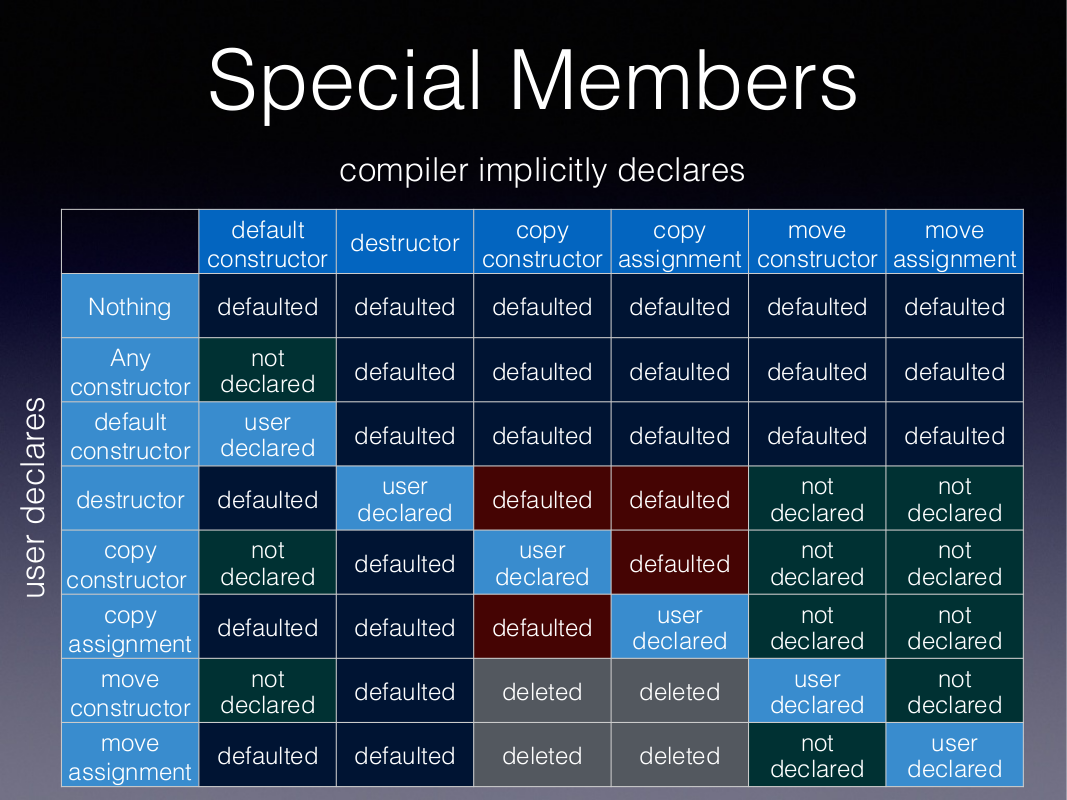
\includegraphics[width=1\textwidth, height=1\textheight, keepaspectratio]{./imgs/rule_of_five.png}
	\caption{Rule of Five}
	\label{fig:rule_of_five}
\end{figure}

%TODO: codice

%TODO: explicit keyword?

% -------------------------- SECTION: MOVE SEMANTICS ---------------------------------

\section{Move Semantics}

\textsf{\small \textbf{Definizione: } Le \textbf{move semantics} permettono, sotto certe condizioni, di trasferire la proprietà delle risorse esterne di qualche oggetto. Questo è importante per due motivi: } \\

\begin{enumerate}
	\item \textsf{\small Trasformare delle costose copie in delle move economiche.}
	\item \textsf{\small Implementare dei tipi di "move-only" sicure; ovvero tipi che per le copie non hanno senso, ma hanno senso per le move.}
	%\item \textsf{\small }
\end{enumerate}

\textsf{\small Per queste è molto importante il concetto di \textbf{lvalue} e di \textbf{rvalue}: } \\

\begin{itemize}
	\item \textsf{\small \textbf{lvalue T\&} : riguardano il copiare.}
	\item \textsf{\small \textbf{rvalue T\&\&} : riguardano il trasferire.}
\end{itemize}

\textsf{\small Per muovere un oggetto useremo \textbf{std::move(oggetto)}. Questa funzione restituisce un \textbf{rvalue} all'oggetto, così che possiamo rubare i dati dall'oggetto in quello nuovo.} \\

\textsf{\small \textbf{std::move(obj)} non cambia il contenuto dell'oggetto, ma \textbf{auto obj2 = std::move(obj)} possibilmente sì.} \\

\subsection{Fallbacks of move semantics}

\begin{enumerate}
	\item \textsf{\small Chiamare la \textbf{std::move()} su un oggetto costante, di solito, non produce effetti.}
	\begin{enumerate}
		\item \textsf{\small Non ha senso rimuovere o muovere/trasferire le risorse di un oggetto costante.}
		%\item \textsf{\small }
	\end{enumerate}
	\item \textsf{\small La semantica della copiatura è un ripiego soltanto se la semantica della copiatura è supportata.}
	\item \textsf{\small Se non c'è implementazione che prenda l'\textbf{rvalue} come argomento allora ci sarà l'ordinario e costante \textbf{lvalue} che verrà usato.}
	\item \textsf{\small Se una funzione non prende un \textbf{rvalue} e \textbf{lvalue} allora un errore a compile-time verrà generato.}
	\item \textsf{\small }
\end{enumerate}

\subsection{syntax vs semantics}

\textsf{\small \textbf{Syntax (Sintassi)}: } \\

\begin{itemize}
	\item \textsf{\small Riguarda le regole per scrivere qualsiasi cosa in un linguaggio di programmazione.}
	\item \textsf{\small Non ha niente a che fare con il significato di ciò che si è scritto.}
	\item \textsf{\small Una dichiarazione è sintatticamente valida se segue tutte le regole.}
	\item \textsf{\small È legata alla grammatica e alla struttura della lingua.}
	\item \textsf{\small Gli errori di sintassi si trovano dopo che il programma è stato eseguito.}
	\item \textsf{\small Alcuni esempi: un punto e virgola mancante. Sono errori semplice da trovare.}
\end{itemize}

\textsf{\small \textbf{Semantics (Semantica)}: } \\

\begin{itemize}
	\item \textsf{\small Riguarda il significato associato alla dichiarazione in una lingua di programmazione.}
	\item \textsf{\small È tutto riguardante il significato della dichiarazione che interpreta il programma.}
	\item \textsf{\small Gli errori sono gestiti a runtime.}
	\item \textsf{\small Si riferisce al significato delle linee di codice associate al linguaggio.}
	\item \textsf{\small Anche se un pezzo di codice ha la sintassi corretta, potrebbe comunque non fare ciò che voleva che facesse. Sono errori un po' più complicati da trovare.}
\end{itemize}

\begin{lstlisting}
	// Codice per dimostrare un errore semantico
	#include <iostream>
	
	int main()
	{
		// Dichiarazione di ritorno prima del cout
		return 0;
		
		std::cout << "Hello World!" << std::endl; // Output: nessun output perché è dopo il return statement.
	}
\end{lstlisting}

\begin{tabular}{|c|c|}
	\hline
	\textbf{Sintassi} & \textbf{Semantica} \\
	\hline
	\textsf{\small Si riferisce alle regole di } & \textsf{\small Si riferisce al significato associato } \\
	\textsf{\small qualsiasi riga di codice.} & \textsf{\small a qualsiasi riga di codice.} \\
	\hline
	\textsf{\small Errori di sintassi. Occorrono a compile time} & \textsf{\small Si riferisce ad un errore semantico. } \\
	\textsf{\small Alcuni esempi: } & \textsf{\small Occorre quando delle righe di codice } \\
	\textsf{\small mancanza di un punto e virgola.} & \textsf{\small sono valide sintatticamente,} \\
	\textsf{\small } & \textsf{\small ma non fanno quello che } \\
	\textsf{\small } & \textsf{\small il programmatore volesse che facessero.} \\
	\hline
\end{tabular}

\subsubsection{Ricapitolando le Move Semantics}

\textsf{\small Ricapitolando: } \\

\begin{itemize}
	\item \textsf{\small Le \textbf{Move Semantics} ci permettono di ottimizzare la copiatura di oggetti. È usato spesso implicitamente (per gli oggetti temporanei) o esplicitamente con \textbf{std::move()}.}
	\item \textsf{\small \textbf{std::move()} significa \emph{non ho più bisogno di questo valore}.}
	\item \textsf{\small Un oggetto segnato con \textbf{std::move()} non è mai parzialmente distrutto. Il distruttore verrà chiamato per distruggere l'oggetto appropriatamente.}
\end{itemize}

% -------------------------- SECTION: CLASSI ASTRATTE --------------------------------

\newpage

%TODO: abstract
%TODO: Pure Virtual

\section{Classi Astratte}

\textsf{\small \textbf{Definizione: } Una \textbf{classe astratta} è una classe generica dove non siamo in grado di implementare tutte le funzioni e che il suo unico scopo è quello di essere ereditata da altre classe che implementeranno le sue funzioni.} \\

\textsf{\small Una classe \textbf{astratta} per essere ritenuta tale deve, almeno, implementare una \textbf{pure virtual function}.} \\

\subsection{Pure Virtual Functions}

\textsf{\small \textbf{Definizione: } Una \textbf{pure virtual function} o \textbf{abstract function} è una funzione virtuale per cui non abbiamo bisogno di scrivere l'implementazione. Le implementazioni verranno poi implementate nelle classe derivate.} \\

\textsf{\small Si dichiara una \textbf{pure virtual function} assegnando 0 alla dichiarazione.} \\

\begin{lstlisting}
	class Test {
		public:
			// Pure Virtual Function
			virtual void show() = 0;
	};
\end{lstlisting}

%TODO: Pure Virtual Destructor

\subsection{Abstract Class}

\textsf{\small \textbf{Definizione: } Proprietà di una \textbf{classe astratta}: } \\

\begin{itemize}
	\item \textsf{\small Possono avere funzioni normali e allo stesso tempo \textbf{pure virtual functions}.}
	\item \textsf{\small Non può essere instanziata, ma si possono creare puntatori e referenze della classe astratta.}
	\item \textsf{\small Le classi astratte sono usate principalmente per \textbf{Upcasting} così che la classe derivata possa usare la sua interfaccia.}
	\item \textsf{\small Se una \textbf{classe astratta} ha una classe derivata, essa deve implementare tutte le \textbf{pure virtual functions} altrimenti diventeranno anch'essi una classe \textbf{astratta}.}
	\item \textsf{\small }
	\item \textsf{\small }
\end{itemize}

\begin{lstlisting}
	#include <iostream>
	
	class Shape {
		public:
			virtual int getArea() = 0;
			void setWidth(int w)
			{
				width = w;
			}
		
			void setHeight(int h)
			{
				height = h;
			}
		
		protected:
			int width;
			int height;
			
	};

	class Rectangle : public Shape {
		public:
			int getArea()
			{
				return width * height;
			}
	};

	class Triangle : public Shape {
		public:
			int getArea()
			{
				return (width * height) / 2;
			}
	};

	int main()
	{
		Rectangle rect;
		Triangle tri;
		
		rect.setWidth(5);
		rect.setHeight(4);
		
		std::cout << "Area rettangolo: " << rect.getArea() << std::endl; // Output: Area Rettangolo: 20
		
		tri.setWidth(5);
		tri.setHeight(4);
		
		std::cout << "Area triangolo: " << tri.getArea() << std::endl; // Output: Area Triangolo: 10
		return 0;
	}
\end{lstlisting}

\subsection{Abstract class vs Interface}

\textsf{\small In un certo senso, possono quasi essere definite come, quelle che in altri linguaggi, si chiamano \textbf{Interfacce}, ovvero un'interfaccia mette semplicemente a disposizione le funzioni, ovvero le loro dichiarazioni e lascia a chi \textbf{implementa} l'interfaccia implementare queste funzioni. Il C++ non ha \textbf{Interfacce}, ma possiamo quasi dire che le \textbf{classi astratte} sono le \textbf{interfacce} del C++.} \break

\textsf{\small Quindi si può simulare un'interfaccia in C++ ponendo tutte le funzioni della classe \textbf{astratta} come \textbf{pure virtual functions}.} \\

% -------------------------- SECTION: ECCEZIONI --------------------------------------

%TODO: try/catch
%TODO: Errori a compile-time ed errori a runtime.
%TODO: throw.
%TODO: std::throw exception

\newpage

\section{Eccezioni}

\textsf{\small \textbf{Definizione: } Cosa sono le \textbf{eccezioni} (in inglese \emph{exceptions})? Le \textbf{eccezioni} sono delle anomalie o condizioni anormali incontrate durante l'esecuzione del programma.} \\

\textsf{\small Il C++ a differenza del C mette a disposizione delle keywords per occuparsi del codice che potrebbe lanciare un'eccezione.} \break

\textsf{\small Durante l'esecuzione del codice diversi errori potrebbero capitare: } \\

\begin{itemize}
	\item \textsf{\small errori nel codice.}
	\item \textsf{\small errori nell'input.}
	\item \textsf{\small altri tipi di errori.}
\end{itemize}

\textsf{\small Quando un errore occorre, C++, di solito, si fermerà e genererà un errore (lancerà un'eccezione).} \\

\subsection{try|catch|throw}

\textsf{\small \textbf{try, catch, throw}: Queste sono le keywords per \emph{Exception Handling} (Gestione delle eccezioni):}

\subsubsection{try}

\textsf{\small Il \textbf{try} ti permette di definire una porzione di codice che verrà testata durante la sua esecuzione. Ovvero se il blocco di codice nel try non lancerà alcuna eccezione allora verrà eseguito il try e poi il codice seguente ad esso, altrimenti verrà eseguito il codice nella clausola \textbf{catch}.} \\

\subsubsection{catch}

\textsf{\small Il \textbf{catch} ti permette di definire un blocco di codice che verrà eseguito se un errore sarà accorso nel \textbf{try}.} \\

\begin{lstlisting}
	try {
		// Blocco di codice del try.
	}catch(NomeEccezione e){
		// Blocco di codice del catch.
	}
\end{lstlisting}

\textsf{\small C'è uno special catch chiamato \emph{catch all} che permette di "catturare" tutte le eccezioni. Si fa in questo modo: \textbf{catch(...) (quindi un catch con l'ellissi, ovvero i tre puntini).}}

\subsubsection{std::throw exception}

\textsf{\small Il \textbf{throw} ti permette di lanciare un'eccezione quando un problema è stato rilevato.} \\

\begin{lstlisting}
	double division(int a, int b)
	{
		if(b == 0)
		{
			std::throw "Divisione per zero!";
		}
		return a/b;
	}

	int main()
	{
		int x = 22;
		int y = 0;
		double z = 0;
		
		try {
			z = division(x,y);
		}catch(const char* msg){
			//std::cerr è lo standard error, lo si può usare per mostrare errori sullo schermo.
			std::cerr << msg << std::endl; //Output: Divisione per zero!
		}
	
		return 0;
	}
\end{lstlisting}

\subsection{Errori a compile time ed errori a runtime}

\textsf{\small Gli errori a \textbf{compile time} sono degli errori che occorrono quando si violano le regole di sintassi del linguaggio, come per esempio: } \\

\begin{itemize}
	\item \textsf{\small Mancanza di una parentesi.}
	\item \textsf{\small Stampare il valore di una variabile senza dichiararla.}
	\item \textsf{\small Mancanza di un punto e virgola.}
\end{itemize}

\textsf{\small Gli errori a \textbf{runtime} sono quegli errori che occorrono durante l'esecuzione del programma dopo che la compilazione sia avvenuta con successo.} \break

\begin{tabular}{|c|c|}
	\hline
	\textbf{Compile-Time Errors} & \textbf{Runtime-Errors} \\
	\hline
	\textsf{\small Errori di sintassi.} & \textsf{\small Non sono rilevati dal compilatore.} \\
	\textsf{\small Prevengono l'esecuzione del codice.} & \textsf{\small Prevengono il codice dalla completa esecuzione.} \\
	\textsf{\small Vengono rilevati dal compilatore } & \textsf{\small Vengono fixati (sistemati) solo dopo} \\
	\textsf{\small e possono essere corretti} & \textsf{\small che il codice viene} \\
	\textsf{\small nel momento della programmazione.} & \textsf{\small eseguito.} \\
	\hline
\end{tabular}

%TODO: Volendo aggiungere immagine "exceptions_recap".
\subsection{Assertions}

\textsf{\small \textbf{Definizione: } Le \textbf{assertions} sono delle dichiarazioni usate per testare delle assunzioni fatte dal programmatore.} \\

\textsf{\small Se la condizione nell'\textbf{assert} fosse valutata falsa, allora il programma fermerebbe l'esecuzione.} \\

\begin{lstlisting}
	#include <assert.h>
	
	int length = 7;
	
	// Un assert per controllare che la variabile length sia maggiore o uguale a 0.
	assert(length >= 0);
	
	// Se l'assert fosse valutato 'false' il programma si fermerebbe e verrebbe mostrato quel messaggio.
	assert(length >= 0 && "La lunghezza non puo' essere negativa");
	
	int x = 0;
	
	// In questo caso verrebbe fermato il programma e verrebbe mostrato il messaggio "x deve essere maggiore di 0"
	assert(x > 0 && "x deve essere maggiore di 0"); 
\end{lstlisting}

% -------------------------- SECTION: OPERAZIONI DI I/O ------------------------------

\newpage

\section{Operazioni di Input/Output}

\textsf{\small \textbf{Definizione: } La libreria standard del C++ mette a disposizioni diverse funzioni per le operazioni di input ed output di dati in streams (flussi di dati), in files, ecc...} \\

\subsection{Input-Output stream}

\textsf{\small \textbf{Definizione: } Le \textbf{stream} sono sequenze, flussi di dati. Quando i dati provengono da dispositivi come tastiere, hard disk, connessioni network sono delle operazioni di \textbf{input}. Quando, invece i dati provengono da dispositivi come schermi, stampanti, disco rigido o una connessione network sono chiamati operazioni di \textbf{output}.} \break

\textsf{\small Il file di intestazione \textbf{<iostream>} definisce le funzioni come \textbf{cin, cout, cerr e clog} che corrispondono allo \emph{standard input}, \emph{standard output}, \emph{un-buffered standard error} e \emph{buffered standard error stream}.} \\

\textsf{\small Per quanto riguarda lo \emph{standard output} i dati vengono inseriti in esso attraverso l'operatore d'inserimento \textbf{<<}.} \break

\textsf{\small È possibile fare questo \emph{chaining} di \textbf{<<} perché l'operatore d'inserzione ritorna una referenza a cout (cout\&).} \\

\begin{lstlisting}
	#include <iostream>
	
	int main()
	{
		int x = 5;
		int y = 8;
		std::cout << "Valore di x: " << x << ", valore di y: " << y << std::endl; // Output: Valore di x: 5, valore di y: 8
		return 0;
	}
\end{lstlisting}

\textsf{\small Tramite \textbf{cin} chiediamo l'input dall'utente. In questa caso usiamo l'operatore di estrazione \textbf{>>}.} \\

\begin{lstlisting}
	#include <iostream>
	
	int main()
	{
		int age;
		
		std::cout << "Inserisci l'età: ";
		std::cin >> age;
		std::cout << "\n La tua età è: " << age << std::endl;
		return 0;
	}
\end{lstlisting}

\textsf{\small \textbf{cerr} è usato per mostrare degli errori sullo schermo. Un-buffered vuol dire che il messaggio non può essere immagazzinato, viene immediatamente mostrato sullo schermo.} \\

\begin{lstlisting}
	#include <iostream>
	
	int main()
	{
		std::cerr << "Si è verificato un errore!";
		return 0;
	}
\end{lstlisting}

\textsf{\small Anche \textbf{clog} come \textbf{cerr} mostra un errore, ma prima lo immagazzina all'interno di un buffer finché non è pieno o viene liberato (usando flush()) e poi verrà mostrato sullo schermo.} \\

\begin{lstlisting}
	#include <iostream>
	
	int main()
	{
		std::clog << "Si è verificato un errore";
		return 0;
	}
\end{lstlisting}

\subsubsection{std::endl vs newline}

\textsf{\small Qual è la differenza tra \textbf{std::endl} ed il carattere di escape newline \textbf{$\backslash$n}?} \\

\textsf{\small \textbf{$\backslash$n} va a capo, mentre \textbf{std::endl} va anch'esso a capo, ma in più ripulisce il buffer, di solito non hai sempre bisogno di farlo e questo ti costerà in termini di \emph{performance}.} \break

\begin{lstlisting}
	#include <iostream>
	
	std::cout << std::endl;
	// std::cout << std::endl è equivalente a:
	std::cout << '\n' << std::flush;
	// Mentre "$\backslash$n" inserisce semplicemente una nuova riga.
	std::cout << "\n";
\end{lstlisting} 

\begin{tabular}{|c|c|}
	\hline
	\textbf{std::endl} & \textbf{\small $\backslash$n} \\
	\hline
	\textsf{\small È un manipolatore.} & \textsf{\small È un carattere.} \\
	\hline
	\textsf{\small Non occupa spazio in memoria.} & \textsf{\small Occupa un byte visto che è un carattere.} \\
	\hline
	\textsf{\small È una keyword e non ha significato } & \textsf{\small Può essere memorizzata } \\
	\textsf{\small se la si memorizza in una stringa.} & \textsf{\small in una stringa e conserva il suo significato.} \\
	\hline
	\textsf{\small Non possiamo scrivere 'endl' in apici.} & \textsf{\small Possiamo scrivere sia '$\backslash$n' sia "$\backslash$n".} \\
	\hline
	\textsf{\small È supportata solo in C++.} & \textsf{\small È supportata sia in C che in C++.} \\
	\hline
	\textsf{\small Continua a ripulire il buffer.} & \textsf{\small Ripulisce il buffer solo alla fine del programma.} \\
	%\textsf{\small } & \textsf{\small } \\
	\hline
\end{tabular}

\textsf{\small Quindi, in conclusione, usare \textbf{$\backslash$n} sembra migliore in termini di prestazioni rispetto \textbf{std::endl} a meno che non sia necessario ripulire il buffer dello stream.} \break

\subsection{Manipolazione degli stream}

%TODO: <iomanip>

\textsf{\small \textbf{Definizione: } I \textbf{manipolatori} sono funzioni che permettono di manipolare \textbf{l'input/output} dello stream. Non vuol dire che modifichiamo la variabile, modifica soltanto lo stream.} \\

\textsf{\small Ci sono diversi tipi di manipolatori: } \\

\begin{enumerate}
	\item \textsf{\small \textbf{Manipolatori senza argomenti}: }
	\begin{itemize}
		\item \textsf{\small \textbf{endl} : serve per andare a capo e dopo averlo fatto ripulisce il buffer dello stream.}
		\item \textsf{\small \textbf{ws} : definito nell'\textbf{istream} e usato per ignorare gli spazi bianchi nella stringa dello stream.}
		\item \textsf{\small \textbf{ends} : inserisce un \emph{null character} nello stream.}
		\item \textsf{\small \textbf{flush} : definito nell'\textbf{ostream} e serve per ripulire l'output stream.}
	\end{itemize}
\end{enumerate}

\begin{lstlisting}
	#include <iostream>
	#include <istream>
	#include <sstream>
	#include <string>
	
	int main()
	{
		// istringstream da <sstream>
		std::istringstream str("   Hello World!");
		
		std::string line;
		
		// Ignora tutti gli spazi bianchi (con std::ws) prima della prima parola.
		std::getline( str >> std::ws, line);
		
		std::cout << line << std::endl;
		
		std::cout << "Test" << std::flush;
		
		std::cout << "A" << "\n";
		std::cout << "B" << std::ends;
		std::cout << "C" << std::endl;
		return 0;
	}
\end{lstlisting}

\begin{enumerate}
	\item \textsf{\small \textbf{Manipolatori con argomenti}: }
	\begin{enumerate}
		\item \textsf{\small \textbf{Alcuni importanti manipolatori in <iomanip>}: }
	\end{enumerate}
		\begin{itemize}
			\item \textsf{\small \textbf{setw(val)} : usato per impostare la larghezza dello spazio negli operatori di output.}
			\item \textsf{\small \textbf{setfill(c)} : usato per riempire lo stream di output con il carattere 'c'.}
			\item \textsf{\small \textbf{setprecision(val)} : Imposta val come nuovo valore di precisione dei valori floating-point.}
			\item \textsf{\small \textbf{setbase(val)} : Per impostare la base dei valori numerici. (es: base 2 (binario), base 16, esadecimale, base 8, ottale, ecc...)}
			\item \textsf{\small \textbf{setioflags(flag)} : Usato per impostare i flag di formato specificati dal parametro di maschera.}
			\item \textsf{\small \textbf{resetiosflags(m)} : Usato per resettare i flags di formato specificati dal parametro di maschera.}
		\end{itemize}
	\begin{enumerate}
		\item[b)] \textsf{\small \textbf{Alcuni manipolatori in <ios>} : }
	\end{enumerate}
		\begin{itemize}
			\item \textsf{\small \textbf{showpos} : Mostra il segno + nei numeri positivi.}
			\item \textsf{\small \textbf{noshowpos} : Non mostra il segno + nei numeri positivi.}
			\item \textsf{\small \textbf{showbase} : Indica la base numerica usati per i valori numerici.}
			\item \textsf{\small \textbf{uppercase} : Mostra le lettere in maiuscolo.}
			\item \textsf{\small \textbf{nouppercase} : Mostra le lettere in minuscolo.}
			\item \textsf{\small \textbf{fixed} : Usa la notazione decimale per i valori floating-point.}
			\item \textsf{\small \textbf{scientific} : Usa la notazione scientifica per i numeri in virgola mobile (floating-point).}
			\item \textsf{\small \textbf{hex} : Legge e scrive valori in esadecimale per i numeri interi e funziona come \emph{setbase(16)}.}
			\item \textsf{\small \textbf{dec} : Legge e scrive valori in decimale per i numeri interi, funziona come \emph{setbase(10)}.}
			\item \textsf{\small \textbf{oct} : Legge e scrive i valori in ottale per i numeri interi, funziona come \emph{setbase(8)}.}
			\item \textsf{\small \textbf{left} : Aggiusta l'output verso sinistra.}
			\item \textsf{\small \textbf{right} : Aggiusta l'output verso destra.}
			%\item \textsf{\small \textbf{} : }
		\end{itemize}
\end{enumerate}

\begin{lstlisting}
	#include <iostream>
	#include <iomanip>
	
	int main()
	{
		int a = 100;
		// Imposto la formattazione.
		std::cout << std::hex << std::left << std::showbase << std::nouppercase;
		
		std::cout << a << std::endl; // Output: 0x64 (esadecimale per 100)
		
		double b = 2001.5251;
		
		// Imposto la formattazione dello stream.
		std::cout << std::setbase(10) << std::right << std::setw(15)
		<< std::setfill('_') << std::showpos
		<< std::fixed << std::setprecision(2);
		
		// Mostro la variabile b
		std::cout << b << std::endl; // Output: \_\_\_\_\_\_\_+2001.53
		
		// Formattazione.
		std::cout << std::scientific << std::uppercase
		<< std::noshowpos << std::setprecision(9);
		
		double c = 201455.2646;
		
		// Stampo la variabile c.
		std::cout << c << std::endl; // Output: 2.014552646E+05
		
		return 0;
	}
\end{lstlisting}

\begin{figure}[ht]
	\centering
	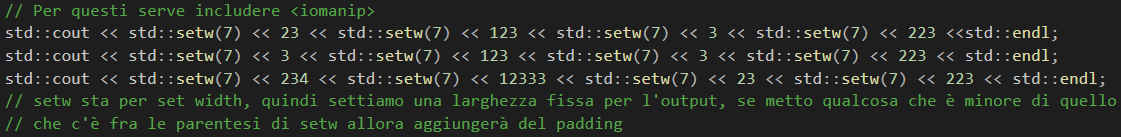
\includegraphics[width=1.2\textwidth, height=1.2\textheight, keepaspectratio]{./imgs/Stream_iomanip_setw.png}
	\caption{Stream iomanip}
	\label{fig:Stream_iomanip_setw}
\end{figure}

\subsection{Operazioni su file}

\textsf{\small \textbf{Definizione: } Per le operazioni di Input/Output sui files avremo bisogno di includere \textbf{fstream}.} \\

\textsf{\small Ci sono diverse modalità di apertura di un file: } \\

\begin{tabular}{|c|c|c|}
	\hline
	\textbf{Costante membra} & \textbf{Significato} & \textbf{Accesso} \\
	\hline
	\textsf{\small \textbf{in*}} & \textsf{\small input} & \textsf{\small File aperto per la lettura: } \\
	\textsf{\small \textbf{}} & \textsf{\small } & \textsf{\small il buffer interno supporta } \\
	\textsf{\small \textbf{}} & \textsf{\small } & \textsf{\small le operazioni di input.} \\
	\hline
	\textsf{\small \textbf{out}} & \textsf{\small output} & \textsf{\small File aperto per la scrittura.} \\
	\hline
	\textsf{\small \textbf{binary}} & \textsf{\small binary} & \textsf{\small Le operazioni vengono eseguite} \\
	\hline
	\textsf{\small \textbf{ate}} & \textsf{\small at end} & \textsf{\small La posizione di output parte dalla fine.} \\
	\hline
	\textsf{\small \textbf{app}} & \textsf{\small append} & \textsf{\small Parte dalla fine e aggiunge contenuti } \\
	\textsf{\small \textbf{}} & \textsf{\small } & \textsf{\small a quelli già presenti.} \\
	\hline
	\textsf{\small \textbf{trunc}} & \textsf{\small truncate} & \textsf{\small Tutti i contenuti } \\
	\textsf{\small \textbf{}} & \textsf{\small } & \textsf{\small che esistevano prima } \\
	\textsf{\small \textbf{}} & \textsf{\small } & \textsf{\small di essere aperto vengono scartati.} \\
	\hline
\end{tabular} \break

\textsf{\small Modalità di apertura di default: } \\

\begin{tabular}{|c|c|}
	\hline
	\textbf{Modalità di apertura di default} & \textbf{} \\
	\hline
	\textsf{\small ifstream} & \textsf{\small ios::in} \\
	\textsf{\small ofstream} & \textsf{\small ios::out} \\
	\textsf{\small fstream} & \textsf{\small ios::in | ios::out} \\
	\hline
\end{tabular}

\begin{lstlisting}
	// Esempio 1
	#include <iostream>
	#include <fstream>
	
	int main()
	{
		std::ofstream myfile;
		myfile.open("nomefile.txt");
		myfile << "Scrivere questa stringa nel file.\n";
		myfile.close();
		return 0;
	}
\end{lstlisting}

\begin{lstlisting}
	// Esempio 2
	#include <iostream>
	#include <fstream>
	
	int main()
	{
		std::string line;
		std::ifstream myfile("nomefile.txt");
		
		if(myfile.is_open())
		{
			while(std::getline(myfile, line))
			{
				std::cout << line << '\n';
			}
		myfile.close();
		} else {
			std::cout << "Impossibile aprire il file" << '\n';
		}
		return 0;
	}
\end{lstlisting}

\textsf{\small P.S. Ricordatevi di chiudere il file una volta che avete finito di utilizzarlo.} \\

\textsf{\small Uno dei modi per ottenere lo spazio occupato da un file: } \\

\begin{figure}[ht]
	\centering
	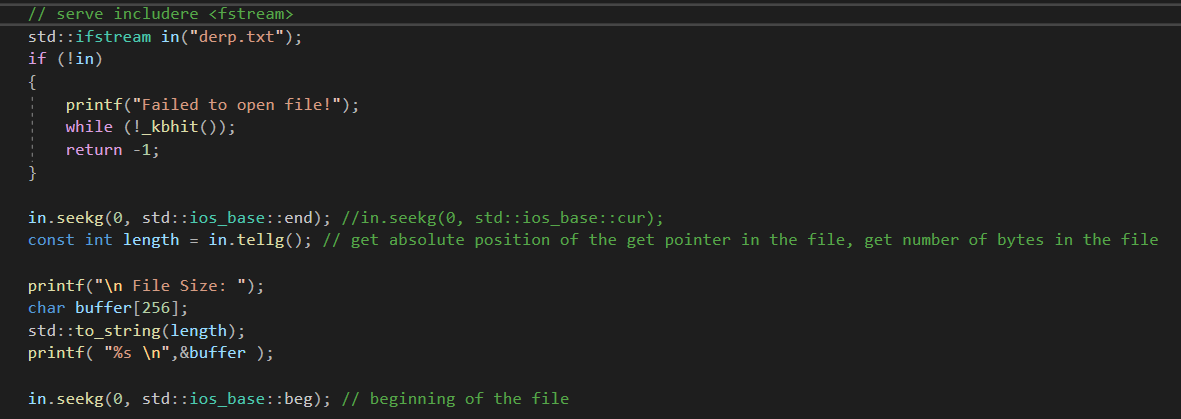
\includegraphics[width=1.2\textwidth, height=1.2\textheight, keepaspectratio]{./imgs/fstream_file_size.png}
	\caption{Ottenere il file size}
	\label{fig:fstream_file_size}
\end{figure}

\begin{figure}[ht]
	\centering
	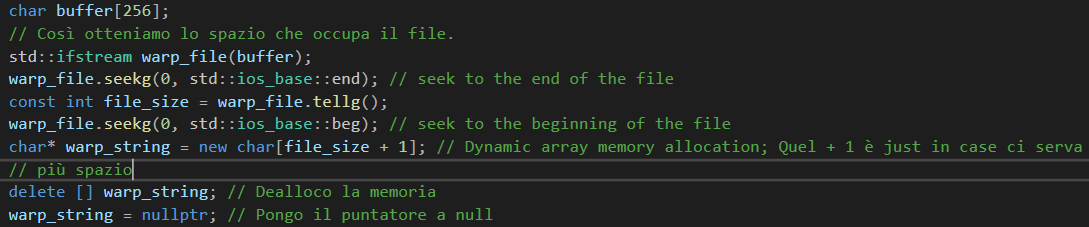
\includegraphics[width=1.2\textwidth, height=1.2\textheight, keepaspectratio]{./imgs/fstream_file_size2.png}
	\caption{Ottenere il file size}
	\label{fig:fstream_file_size2}
\end{figure}

% -------------------------- SECTION: STD::CHRONO ------------------------------------

\newpage

\section{std::chrono}

\textsf{\small \textbf{Definizione: } La libreria \textbf{chrono} è usata per occuparsi delle date e del tempo. Questa libreria è progettata col fatto che i timers e gli orologi potrebbero essere diversi su sistemi operativi differenti.} \\

\textsf{\small Fornisce una \emph{precisione neutrale}, attraverso la separazione le durate e il tempo.} \\

\textsf{\small Tutti gli elementi di questo header non sono definiti sotto il namespace std, ma sotto il \textbf{std::chrono namespace}.} \break

\textsf{\small Si occupa del tempo attraverso principalmente 3 concetti: } \\

\begin{itemize}
	\item \textsf{\small \textbf{Duration (Durata)} : Un oggetto durata esprime un intervallo di tempo come 3 minuti, 3 ore, 3 millisecondi, ecc.. Per esempio 33 secondi potrebbe essere rappresentato dalla durata di 33 ticks ciascuno di 1 secondo.}
	\item \textsf{\small \textbf{Clock (Orologio)} : Un orologio consiste in un punto di partenza (o epoch) e un tick rate.}
	\item \textsf{\small \textbf{Time point (Punto nel tempo)} : Un oggetto di tipo \emph{time\_point} esprime un punto nel tempo relativo ad un epoch di un clock. Internamente, l'oggetto memorizza un oggetto di tipo durata (\emph{duration}) e usa il clock come referenza per via del suo epoch.}
\end{itemize}

\subsection{Duration}

\begin{lstlisting}
	#include <iostream>
	#include <chrono>	
	
	int main ()
	{
		using namespace std::chrono;
		
		// std::chrono::milliseconds è una
		// instanzione di std::chrono::duration: - 1 secondo
		
		milliseconds mil(1000);
		
		mil = mil*60;
		
		std::cout << "durata (in periodi): ";
		std::cout << mil.count() << " millisecondi.\n"; // Output: durata (in periodi): 60000 millisecondi.
		
		std::cout << "durata (in secondi): ";
		std::cout << (mil.count() * milliseconds::period::num /
		milliseconds::period::den);
		std::cout << " secondi.\n"; // Output: durata (in secondi): 60 secondi.
		
		return 0;
	}
\end{lstlisting}

\subsection{Clock}

\textsf{\small Ci sono 3 diversi tipi di clock (orologi): } \\

\begin{itemize}
	\item \textsf{\small \textbf{system\_clock} : È il tempo corrente in base al sistema operativo (quello che vediamo nella barra dei comandi). È scritto come \emph{std::chrono::system\_clock}.}
	\item \textsf{\small \textbf{steady\_clock} : È un orologio monotonic (monotonico, uniforme) che non può essere aggiustato, regolato. Va ad un rate uniforme. È scritto come \emph{std::chrono::steady\_clock}.}
	\item \textsf{\small \textbf{high\_resolution\_clock} : Fornisce il periodo di tick più piccolo possibile. È scritto come \emph{std::chrono::high\_resolution\_clock}.}
\end{itemize}

\subsection{Time point}

\subsubsection{Calcolare il tempo di esecuzione di un blocco di codice}

\begin{lstlisting}
	// Esempio 1 Implementazione 1 per calcolare il tempo che un blocco di codice ci mette per essere eseguito.
	#include <iostream>
	#include <chrono>
	#include <ctime>
	
	long fibonacci(unsigned n)
	{
		if (n < 2) return n;
		return fibonacci(n-1) + fibonacci(n-2);
	}
	
	int main()
	{
		// time point e system\_clock
		std::chrono::time_point<std::chrono::system_clock> start, end;
		
		start = std::chrono::system_clock::now();
		std::cout << "f(42) = " << fibonacci(42) << '\n'; // Output: f(42) = 267914296
		end = std::chrono::system_clock::now();
		
		std::chrono::duration<double> elapsed_seconds = end - start;
		std::time_t end_time = std::chrono::system_clock::to_time_t(end);
		
		std::cout << "Finito di eseguire il " << std::ctime(&end_time)
		<< "tempo passato: " << elapsed_seconds.count() << "s\n"; // Output: Finito di eseguire il Sun Mar 13 22:53:59 2022 elapsed time: 2.71703s
	}
\end{lstlisting}

\textsf{\small Esempio 2 Implementazione 2 per calcolare il tempo di esecuzione di un blocco di codice: } \\

\begin{figure}[ht]
	\centering
	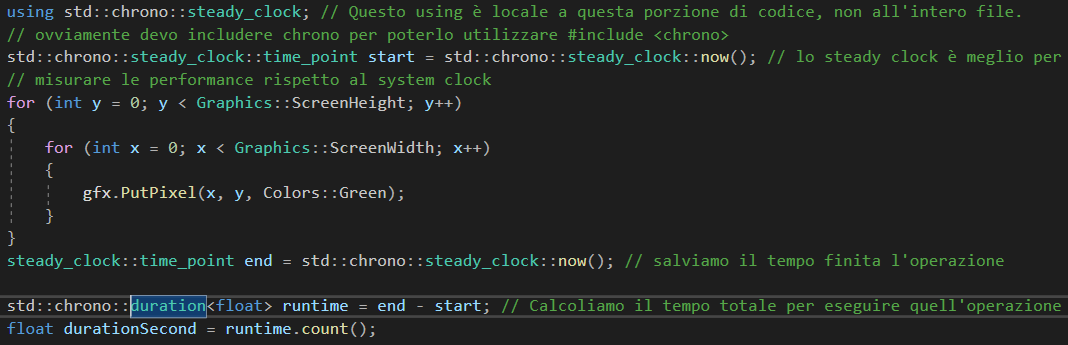
\includegraphics[width=1.2\textwidth, height=1.2\textheight, keepaspectratio]{./imgs/chrono_steady_clock_per_misurare_il_tempo_tra_una_operazione_e_l_altra_col_using.png}
	\caption{Calcolo tempo trascorso per eseguire un blocco di codice}
	\label{fig:chrono_steady_clock_per_misurare_il_tempo_tra_una_operazione_e_l_altra_col_using}
\end{figure}

% --------------------- SECTION: GENERATORI DI NUMERI CASUALI ------------------------

\newpage

\section{Generatori di numeri pseudo-casuali}

\textsf{\small \textbf{Definizione: } I \textbf{generatori di numeri pseudo-casuali} ci permettono di generare dei numeri che sembrano casuali. } \\

\subsection{Numeri casuali come in C}

\textsf{\small In C e di conseguenza in C++ si può utilizzare \textbf{rand()} e \textbf{srand()} importando \textbf{stdlib.h} in C e \textbf{<cstdlib>} in C++.} \\

\begin{lstlisting}
	// Esempio 1
	#include <iostream>
	#include <cstdlib>
	
	// Questo programma genererà sempre la stessa sequenza di numeri ad ogni esecuzione.
	int main()
	{
		int number;
		for(int i = 0; i < 3; i++)
		{
			number = rand();
			std::cout << number << std::endl;
		}
		return 0;
	}
\end{lstlisting}

\textsf{\small Per generare un numero compreso in un range (raggio: tra due numeri) usiamo l'operatore modulo e il numero a cui può arrivare.} \\

\begin{lstlisting}
	// Esempio 2
	#include <iostream>
	#include <cstdlib>
	
	// Questo programma genererà un numero nel range 25 e 50.
	int main()
	{
		int max = 50;
		int min = 25;
		int range = max - min + 1;
		
		int num = rand() % range + min;
		return 0;
	}
\end{lstlisting}

\textsf{\small \textbf{Definizione: } Il \textbf{seed} (seme) è il punto d'inizio della sequenza, può essere cambiato affinché la sequenza di numeri generati sia diversa.} \\

\textsf{\small Nel prossimo esempio usiamo il tempo corrente per generare un \emph{seed} (un seme). Usiamo \textbf{srand} per impostare il seme. } \\

\begin{lstlisting}
	// Esempio 3
	#include <iostream>
	#include <cstdlib>
	#include <time.h>
	
	// Questo programma genererà un numero nel range 25 e 50.
	int main()
	{
		
		constexpr int NUM_OF_NUMBERS = 3;
		
		int number;
		
		// Usiamo srand per settare il seed ed usiamo il tempo corrente in questo caso come parametro del seed.
		std::srand(time(0));
		
		for(int i = 0; i < NUM_OF_NUMBERS; i++)
		{
			number = rand();
			std::cout << number << std::endl;
		}
		return 0;
	}
\end{lstlisting}

\subsection{Cosa vuol dire e perché pseudo-random?}

\textsf{\small Gli \textbf{pseudorandom number generator} (\emph{PRNG}), anche chiamati \textbf{deterministic random bit generator} (\emph{DRBG}, ovvero generatori di bit casuali deterministici) sono degli algoritmi per generare sequenze di numeri le quali proprietà sono simili a quelle delle sequenze di numeri casuali.} \\

\textsf{\small I \emph{PRNG} non generano vere sequenze casuali perché è completamente determinato da un numero di partenza chiamato \emph{seed} (seme).} \break

\textsf{\small Quindi è chiamato "\emph{pseudo}" casuale perché l'algoritmo può ripetere la sequenza e quindi i numeri non sono propriamente casuali.} \\

\subsection{I vari tipi di generatori}

\textsf{\small \textbf{Definizione: } Nell'header \textbf{<random>} sono contenuti diversi generatori di numeri pseudo-casuali e diverse distribuzioni:} \\

\begin{itemize}
	\item \textsf{\small \textbf{Generatori} : oggetti che generano numeri distribuiti uniformemente.}
	\item \textsf{\small \textbf{Distribuzioni} : oggetti che trasformano sequenze di numeri generati da un generatore in sequenze di numeri che seguono una specifica distribuzione variabili e casuale, come: uniforme, normale, binomiale.}
\end{itemize}

\begin{enumerate}[I]
	\item \textsf{\small \textbf{Pseudo-random number engines} : usano un algoritmo per generare numeri casuali basati su un seme iniziale. Questi sono: }
\end{enumerate}

\begin{figure}[ht]
	\centering
	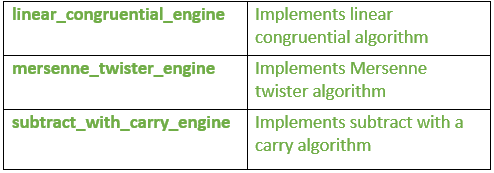
\includegraphics[width=1.2\textwidth, height=1.2\textheight, keepaspectratio]{./imgs/random-number-engines.png}
	\caption{Motori di numeri pseudo-casuali}
	\label{fig:random-number-engines}
\end{figure}

\begin{enumerate}
	\item \textsf{\small \textbf{linear\_congruential\_engine} : è il più semplice nella \textbf{STL} (\emph{Standard Template Library}) che genera numeri interi senza segno.}
\end{enumerate}

\begin{lstlisting}
	#include <iostream>
	#include <chrono>
	#include <random>
	
	int main()
	{
		// Trova il tempo tra il clock del sistema (tempo corrente) e l'epoch del clock (data e tempo relativi quando il timestamp di un clock di un computer sono determinati).
		unsigned seed = std::chrono::system_clock::now().time_since_epoch().count();
		
		std::minstd_rand0 generator(seed);
		
		std::cout << generator() << "è un numero casuale tra ";
		std::cout << generator.min() << " e " << generator.max();
		return 0;
	}
\end{lstlisting}

\begin{enumerate}
	\item[2.] \textsf{\small \textbf{mersenne\_twister\_engine} : È un motore di numeri casuali basati sull'algoritmo \emph{Mersenne Twister}. Produce dei numeri senza segno di alta qualità nell'intervallo [$0, (2^w)-1]$. dove \emph{w = size della parola (word)}.} \\
\end{enumerate}

\begin{lstlisting}
	// Esempio 1
	#include <iostream>
	#include <chrono>
	#include <random>
	
	int main()
	{
		unsigned seed = std::chrono::system_clock::now().time_since_epoch().count();
		
		std::mt19937 generator(seed);
		
		std::cout << generator() << " è un numero casuale tra ";
		
		std::cout << generator.min() << " e " << generator.max();
		return 0;
	}
\end{lstlisting}

\begin{lstlisting}
	// Esempio 2
	#include <iostream>
	#include <chrono>
	#include <random>
	
	int randomNumberGenerator(int limit)
	{
		// generatore di numeri interi casuali con distribuzione uniforme che produce numeri casuali non deterministici.
		std::random_device rd;
		
		// Generatore pseudo-random con l'algoritmo Mersenne Twister di numeri a 32 bit con uno spazio di stato di 19937 bits.
		std::mt19937 rng(rd());
		
		// Distribuzione uniforme
		std::uniform_int_distribution<> dis(1, limit);
		return dis(rng);
	}
	
	int main()
	{
		int limit = 100;
		std::cout << randomNumberGenerator(limit) << std::endl;
		return 0;
	}
\end{lstlisting}

\begin{enumerate}
	\item[3.] \textsf{\small \textbf{subtract\_with\_carry\_engine} : È un motore di generazione di numeri pseudo-casuali che produce numeri interi senza segno. L'algoritmo usato è il \emph{generatore di fibonacci} con una sequenza di stati di r elementi, più uno per il carry (il resto).} \\
\end{enumerate}

\begin{lstlisting}
	#include <iostream>
	#include <chrono>
	#include <random>
	
	int main()
	{
		unsigned seed = std::chrono::system_clock::now().time_since_epoch().count();
		
		std::subtract_with_carry_engine<unsigned, 24, 10, 24> generator(seed);
		
		std::cout << generator() << " è un numero casuale tra ";
		
		std::cout << generator.min() << " e " << generator.max();
		return 0;
	}
\end{lstlisting}

\begin{enumerate}[I]
	\item[II] \textsf{\small \textbf{Random number generator} : È un generatore di numeri casuali che produce numeri casuali non deterministici.} \\
\end{enumerate}

\begin{lstlisting}
	#include <iostream>
	#include <random>
	
	int main ()
	{
		std::random_device rd;
		
		std::cout << "default random_device caratteristiche:" << std::endl;
		
		std::cout << "minimo: " << rd.min() << std::endl;
		
		std::cout << "massimo: " << rd.max() << std::endl;
		
		std::cout << "entropia: " << rd.entropy() << std::endl;
		
		std::cout << "un numero casuale: " << rd() << std::endl;
		
		return 0;
	}
\end{lstlisting}

\begin{enumerate}[I]
	\item[III] \textsf{\small \textbf{Pseudo-random number engines (instantions)} : Questi sono particolari instanzioni di motori di generatori e adattatori: } \\
\end{enumerate}

\begin{figure}[ht]
	\centering
	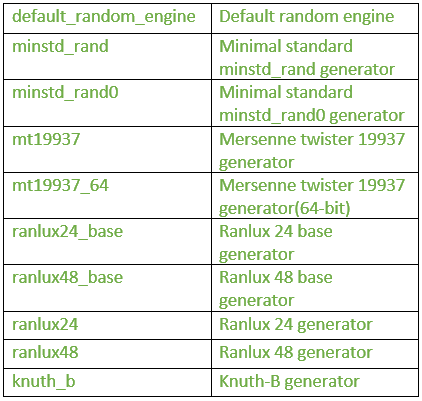
\includegraphics[width=1\textwidth, height=1\textheight, keepaspectratio]{./imgs/pseudo-random-number-engines.png}
	\caption{Motori di numeri pseudo casuali}
	\label{fig:pseudo-random-number-engines}
\end{figure}

\begin{enumerate}
	\item \textsf{\small \textbf{default\_random\_engine} : Questo è una classe che genera numeri pseudo-casuali.} \\
\end{enumerate}

\begin{lstlisting}
	#include <iostream>
	#include <chrono>
	#include <random>
	
	int main()
	{
		
		unsigned seed = std::chrono::system_clock::now().time_since_epoch().count();
		
		// minstd\_rand0 è un standard linear\_congruential\_engine
		std::minstd_rand0 generator(seed);
		
		std::cout << generator() << " è un numero casuale tra ";
		
		std::cout << generator.min() << " e " << generator.max();
		
		return 0;
	}
\end{lstlisting}

\begin{enumerate}
	\item[2.] \textsf{\small \textbf{minstd\_rand} : Genera numeri pseudo casuali. È simile al linear congruential generator.} \\
\end{enumerate}

\begin{lstlisting}
	#include <iostream>
	#include <chrono>
	#include <random>
	
	int main()
	{
		
		unsigned seed = chrono::system_clock::now().time_since_epoch().count();
		
		// minstd\_rand0 è un standard
		//linear\_congruential\_engine
		std::minstd_rand0 generator(seed);
		
		std::cout << generator() << " è un numero casuale tra ";
		
		std::cout << generator.min() << " e " << generator.max();
		
		return 0;
	}
\end{lstlisting}

\begin{enumerate}
	\item[3.] \textsf{\small \textbf{mt19937} : È il generatore \emph{Mersenne Twister} 19937. È un generatore di numeri a 32 bit con uno spazio di stato di 19937 bits.} \\
\end{enumerate}

\begin{enumerate}
	\item[4.] \textsf{\small \textbf{ranlux24\_base} : È un generatore \emph{Ranlux base 24}. È un generatore pseudo casuale che sottrae con il resto di numeri a 24-bit, generalmente usato come base per il generatore \emph{ranlux24}.} \\
\end{enumerate}

\begin{lstlisting}
	#include <iostream>
	#include <chrono>
	#include <random>
	
	int main ()
	{	
		unsigned seed = std::chrono::system_clock::now().time_since_epoch().count();
		std::subtract_with_carry_engine<unsigned,24,10,24> generator(seed);
		
		std::cout << generator() << " è un numero casuale tra ";
		
		std::cout << generator.min() << " e " << generator.max();
		
		return 0;
	}
\end{lstlisting}

\begin{enumerate}[I]
	\item[IV] \textsf{\small \textbf{Engine Adaptors}} \\
\end{enumerate}

\begin{enumerate}
	\item \textsf{\small \textbf{discard\_block\_engine} : È una classe template che adatta un motore di generatore di numeri pseudo-casuali attraverso il solo utilizzo di 'r' elementi di ogni blocco e 'p' elementi dalla sequenza che produce, scartando il resto. L'adattatore tiene un contatore interno per tenere traccia di quanti elementi sono stati prodotti nel blocco corrente.}
\end{enumerate}

\textsf{\small I generatori \textbf{ranlux24} e \textbf{ranlux48} adattano un \textbf{subtract\_with\_carry\_engine} usando questo adattatore.} \\

\begin{lstlisting}
	#include <iostream>
	#include <chrono>
	#include <random>
	
	int main ()
	{
		unsigned seed = std::chrono::system_clock::now().time_since_epoch().count();
		
		// ranlux24 è un standard instantitation
		// del discard\_block\_engine:
		std::ranlux24 generator(seed);
		
		std::cout << generator() << " è un numero casuale tra ";
		
		std::cout << generator.min() << " e " << generator.max();
		
		return 0;
	}
\end{lstlisting}

\begin{enumerate}
	\item[2.] \textsf{\small \textbf{indipendent\_bits\_engine} : È un adattatore che adatta un motore di generatore di numeri casuali per produrre numeri con uno specifico numero di bits (w).}
\end{enumerate}

\begin{lstlisting}
	#include <iostream>
	#include <chrono>
	#include <cstdint>
	#include <random>
	
	int main ()
	{
		unsigned seed = std::chrono::system_clock::now().time_since_epoch().count();
		
		// independent\_bits\_engine
		std::independent_bits_engine<mt19937,64,uint_fast64_t> generator(seed);
		
		std::cout << generator() << " è un numero casuale tra ";
		
		std::cout << generator.min() << " e " << generator.max();
		
		return 0;
	}
\end{lstlisting}

\begin{enumerate}
	\item[3.] \textsf{\small \textbf{shuffle\_order\_engine} : È un adattatore che adatta un motore di generatore di numeri pseudo-casuali così che i numeri siano ottenuti in una sequenza differente.}
\end{enumerate}

\textsf{\small L'oggetto mantiene un buffer di k numeri generati internamente e quando richiesti restituisce alcuni selezionati casualmente nel buffer, rimpiazzandolo con un valore ottenuto dalla base del motore.} \\

\begin{lstlisting}
	#include <iostream>
	#include <chrono>
	#include <random>
	
	int main ()
	{
		unsigned seed = std::chrono::system_clock::now().time_since_epoch().count();
		
		// ranlux24 è un standard instantitation
		// del discard\_block\_engine:
		ranlux24 generator (seed);
		
		std::cout << generator() << " è un numero casuale tra ";
		
		std::cout << generator.min() << " e " << generator.max();
		
		return 0;
	}
\end{lstlisting}

% ------------------------ SECTION: MAP, SET, PAIR, HASH TABLE -----------------------

\newpage

\section{Map | Set | Pair | Hash Table}

\textsf{\small \textbf{Definizione: } Ora tratteremo delle \textbf{map, set, pair, hash table} che sono contenitori molto utili per poter eseguire delle operazioni sui loro elementi.} \\

\subsection{Map}

\textsf{\small \textbf{Definizione: } Le \textbf{mappe} sono dei contenitori associativi, ovvero che ogni elemento ha una chiave e un valore mappato. Non ci possono essere due valori con la stessa chiave.} \\

\textsf{\small Per poter utilizzare le \textbf{mappe} includiamo l'header \textbf{<map>}.} \\

\textsf{\small Quindi ricapitolando in una mappa ci sono una sequenza di (chiave, valore) \{\{\textbf{chiave}:\textbf{valore}\}, \{\textbf{chiave}:\textbf{valore}\}, \{\textbf{chiave}:\textbf{valore}\}, \{\textbf{chiave}:\textbf{valore}.\}\}} \\

\begin{lstlisting}
	#include <iostream>
	#include <map>
	
	int main()
	{
		std::map<char, int> map;
		
		map.insert('a', 0);
		map.insert('b', 1);
		map.insert('c', 2);
		
		std::cout << "map size: " << map.size() << std::endl; // Output: map size: 3
		
		map.clear();
		
		std::cout << "map size dopo clear: " << map.size() << std::endl; // Output: map size dopo clear: 0
		
		std::map<std::string, int> myMap = {
			{"one", 1}, {"two", 2}, {"three", 3}
		};
	
		for(auto& i : myMap)
		{
			std::cout << i.first << ": " << i.second << std::endl;
			// Output: one: 1
			// Output: two: 2
			// Output: three: 3
		}
		
		return 0;
	}
\end{lstlisting}

\subsubsection{unordered\_map} 

\textsf{\small \textbf{Definizione: } Una \textbf{unordered\_map} è una mappa non ordinata, quindi i suoi elementi sono memorizzati in nessun tipo di ordine particolare, ma sono piazzati a caso.} \\

\textsf{\small Una \textbf{unordered\_map} è implementata usando una \emph{Hash Table}, quindi le performance della struttura dati dipendono dalla funzione hash.} \\

\textsf{\small Per poter utilizzare l'\textbf{unordered\_map} è necessario includere il file di intestazione: \textbf{<unordered\_map>}.} \\

\begin{figure}[ht]
	\centering
	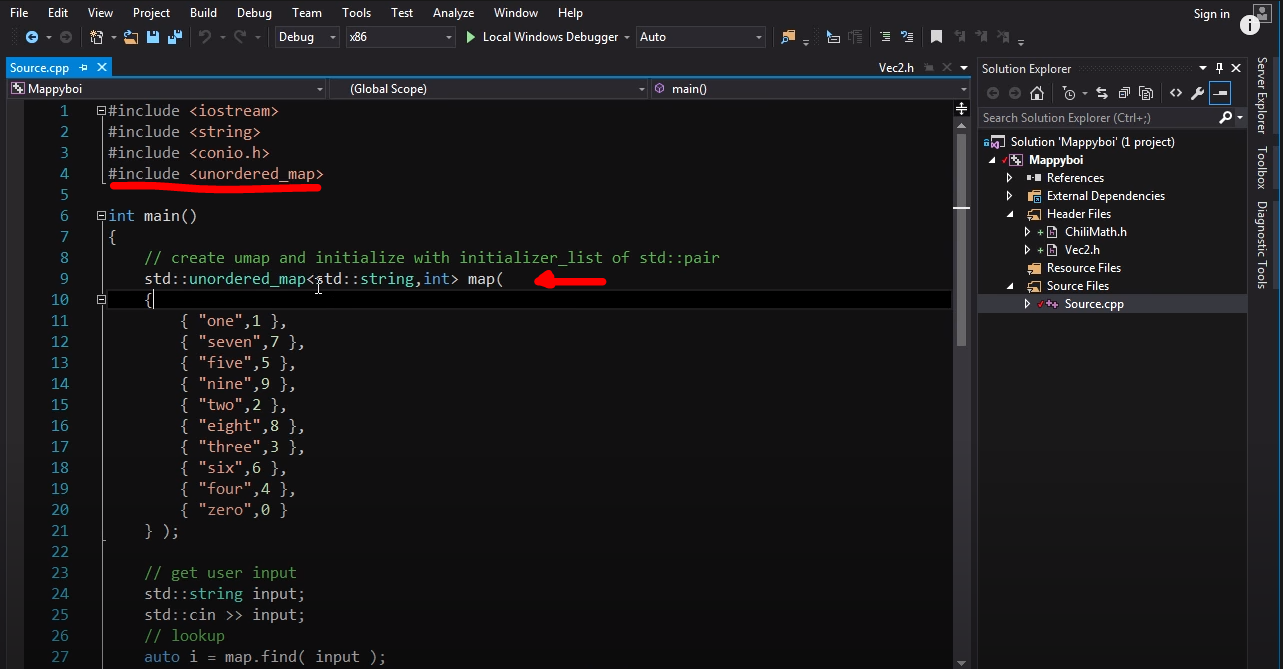
\includegraphics[width=1.2\textwidth, height=1.2\textheight, keepaspectratio]{./imgs/unordered_map_include_unordered_map_initialize_it.png}
	\caption{unordered\_map}
	\label{fig:unordered_map_include_unordered_map_initialize_it}
\end{figure}

\begin{figure}[ht]
	\centering
	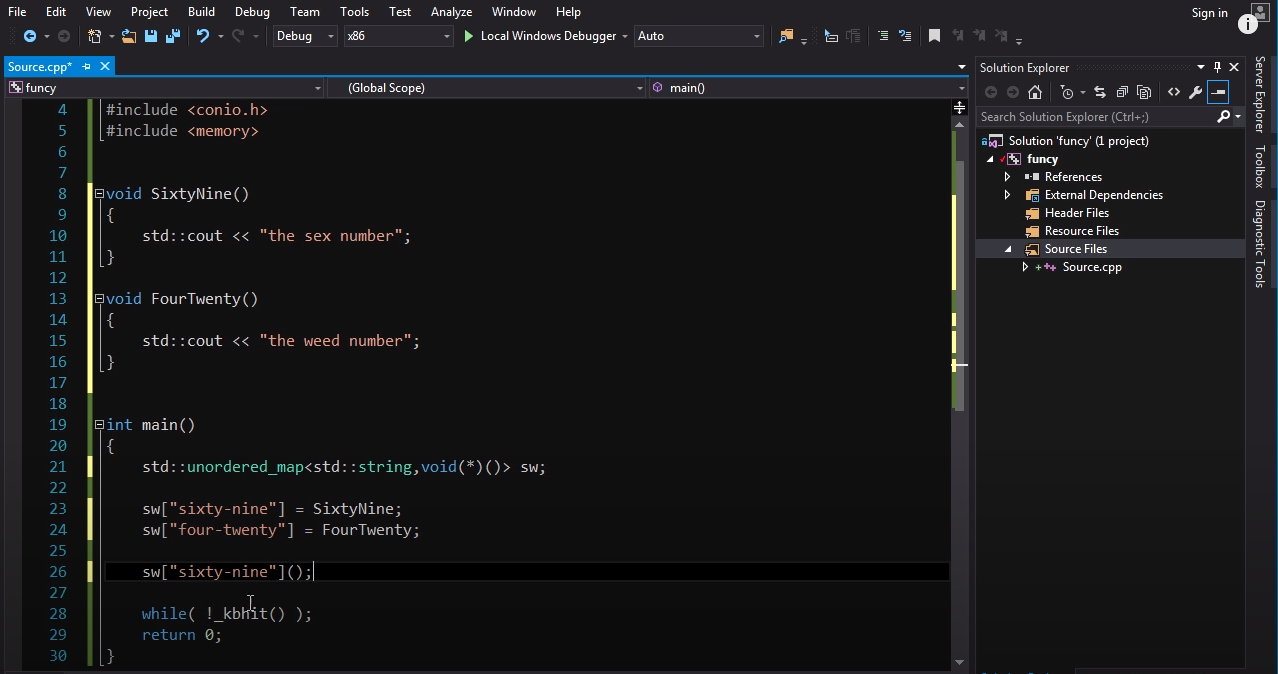
\includegraphics[width=1.2\textwidth, height=1.2\textheight, keepaspectratio]{./imgs/function_pointers_unordered_map_pointer_to_a_function.png}
	\caption{unordered\_map function pointer}
	\label{fig:function_pointers_unordered_map_pointer_to_a_function}
\end{figure}

\subsection{unordered\_map function pointer}

\begin{figure}[H]
	\centering
	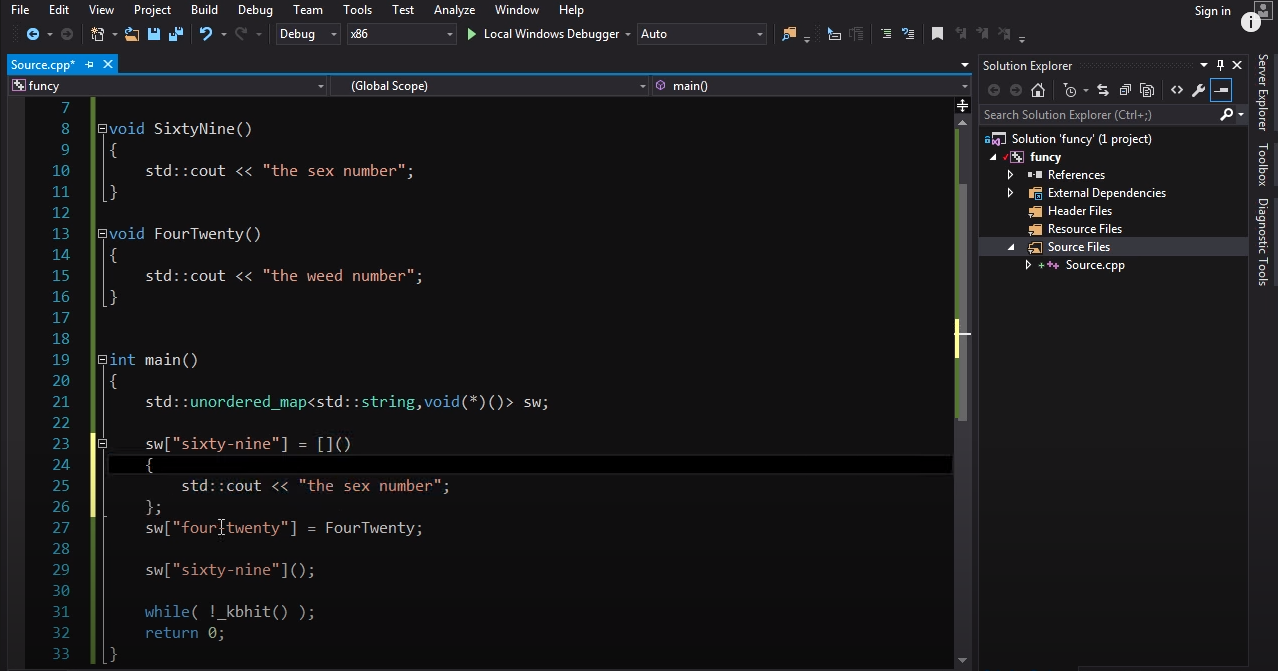
\includegraphics[width=1.2\textwidth, height=1.2\textheight, keepaspectratio]{./imgs/function_pointers_unordered_map_pointer_to_a_function_lambda_function.png}
	\caption{unordered\_map function pointer}
	\label{fig:function_pointers_unordered_map_pointer_to_a_function_lambda_function}
\end{figure}

\begin{figure}[H]
	\centering
	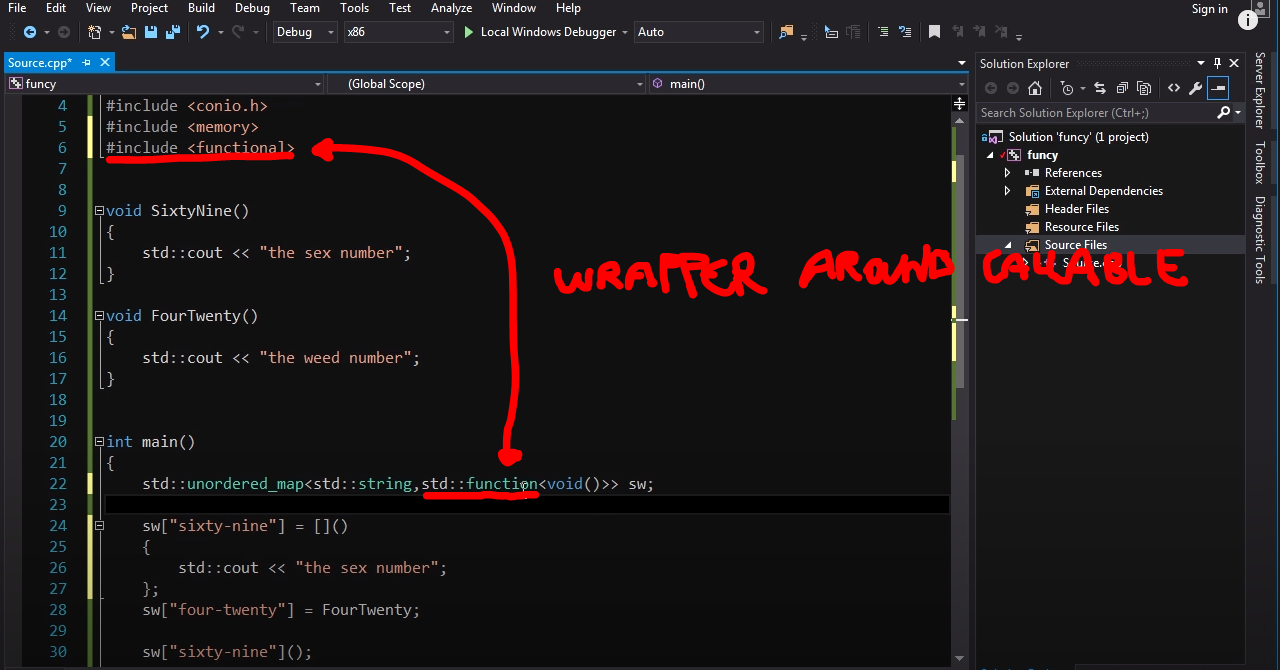
\includegraphics[width=1.2\textwidth, height=1.2\textheight, keepaspectratio]{./imgs/function_pointers_unordered_map_functional_std_function.png}
	\caption{unordered\_map function pointer}
	\label{fig:function_pointers_unordered_map_functional_std_function}
\end{figure}


\begin{figure}[H]
	\centering
	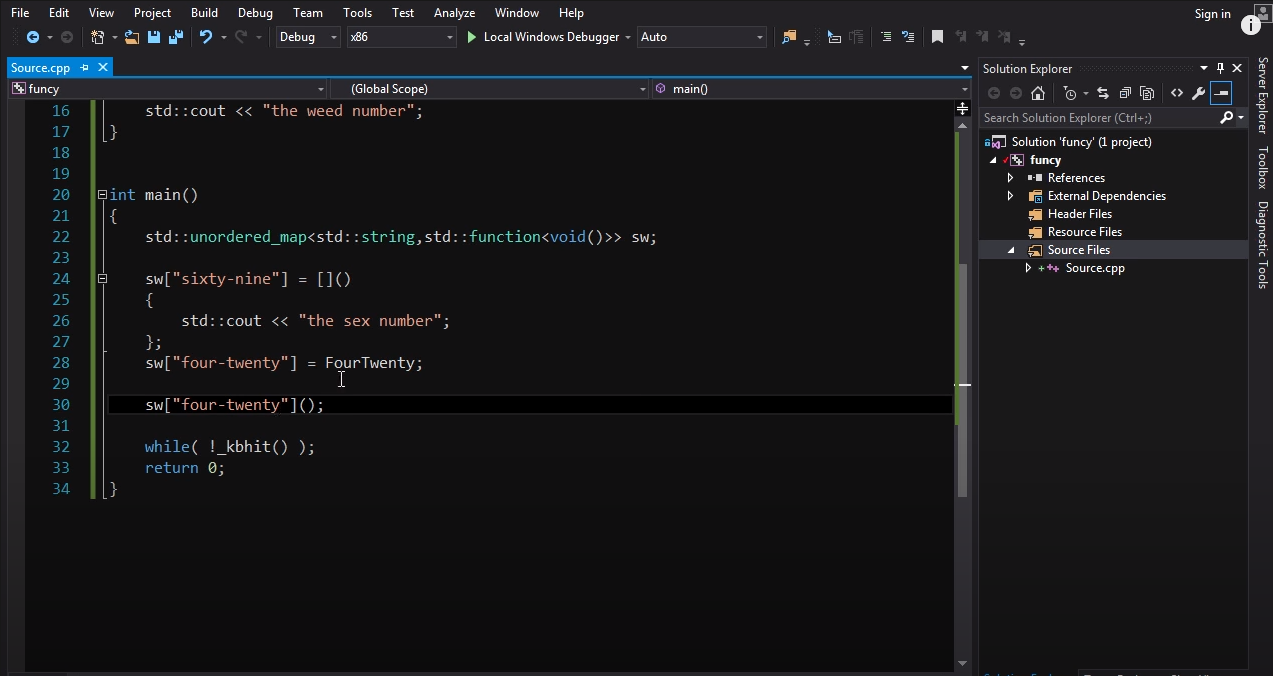
\includegraphics[width=1.2\textwidth, height=1.2\textheight, keepaspectratio]{./imgs/function_pointers_unordered_map_functional_std_function2.png}
	\caption{unordered\_map function pointer}
	\label{fig:function_pointers_unordered_map_functional_std_function2}
\end{figure}

\begin{figure}[H]
	\centering
	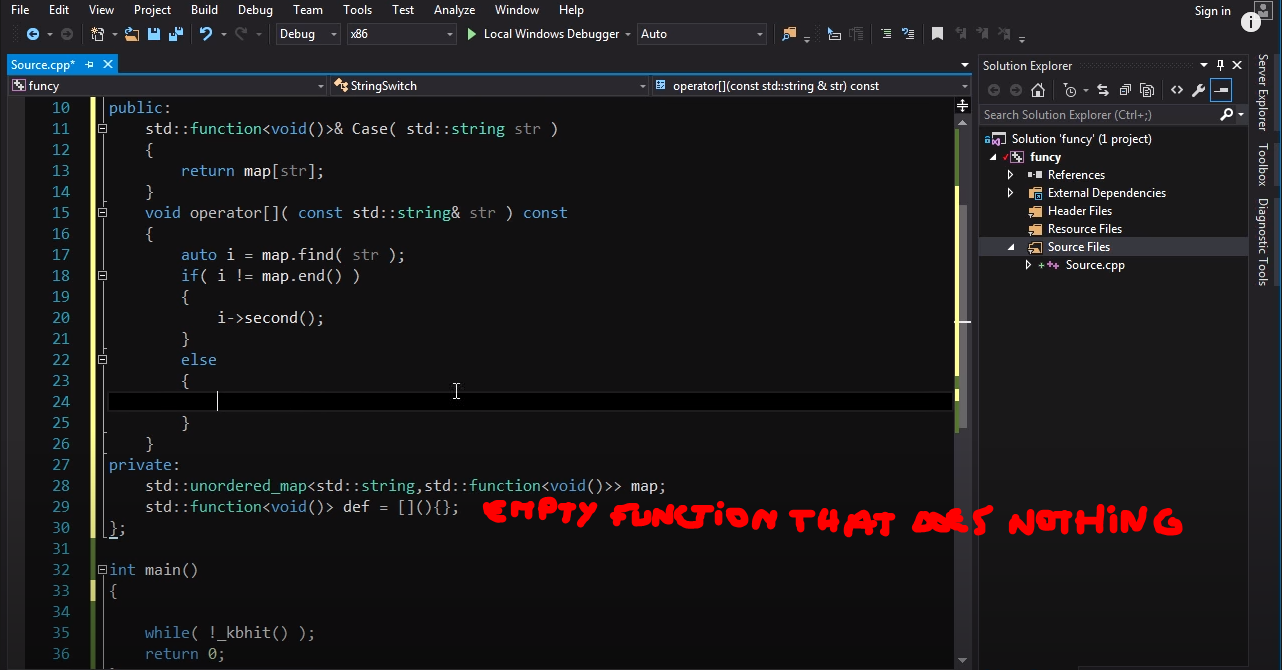
\includegraphics[width=1.2\textwidth, height=1.2\textheight, keepaspectratio]{./imgs/function_pointers_unordered_map_functional_std_function3.png}
	\caption{unordered\_map function pointer}
	\label{fig:function_pointers_unordered_map_functional_std_function3}
\end{figure}

\subsubsection{multimap}

\textsf{\small \textbf{Definizione: } Una \textbf{multimap} è simile ad una \textbf{mappa}, ma con l'aggiunta che molteplici elementi possono avere le stesse chiavi. Inoltre, in questo caso, le coppie chiave-valore non devono essere per forza uniche. Inoltre, nelle \textbf{multimap} le chiavi sono sempre memorizzate in ordine.} \\

\begin{lstlisting}
	#include <iostream>
	#include <map>
	
	int main()
	{
		std::multimap<char, int> m1 = {
			{'a', 1},
			{'a', 2},
			{'b', 3},
			{'c', 4},
			{'c', 5},
		};
		
		std::multimap<char, int>m2(m1.begin(), m1.end());
		
		std::cout << "La Multimap contiene i seguenti elementi:" << std::endl;
		for (auto it = m2.begin(); it != m2.end(); ++it)
		std::cout << it->first << " = " << it->second << std::endl;
		
		//Output: La multimap contiene i seguenti elementi: 
		//Output: a = 1
		//Output: a = 2
		//Output: b = 3
		//Output: c = 4
		//Output: c = 5
		
		return 0;
	}
\end{lstlisting}

\subsection{Set}

\textsf{\small \textbf{Definizione: } I \textbf{set} (insiemi in italiano) è un contenitore associativo nel quale gli elementi devono essere unici. Gli elementi dell'insieme non possono essere modificati una volta nel container, quindi sono sempre \textbf{const}.} \\

\textsf{\small Per usare gli insieme è necessario includere l'header \textbf{<set>}.} \\

\textbf{Proprietà: } \\

\begin{enumerate}
	\item \textsf{\small Il \textbf{set} memorizza gli elementi in ordine.}
	\item \textsf{\small Tutti gli elementi in un \textbf{set} hanno valori unici.}
	\item \textsf{\small I valori del \textbf{set} non possono essere modificati, quindi sono \textbf{immutable} (immutabili).}
	\item \textsf{\small I \textbf{set} utilizzano la \textbf{Binary search tree}.}
	\item \textsf{\small I valori in un set sono \textbf{non indicizzati}.}
\end{enumerate}

\textsf{\small Per memorizzare gli elementi in maniera non ordinata c'è \textbf{unordered\_set()}.} \\

\begin{figure}[H]
	\centering
	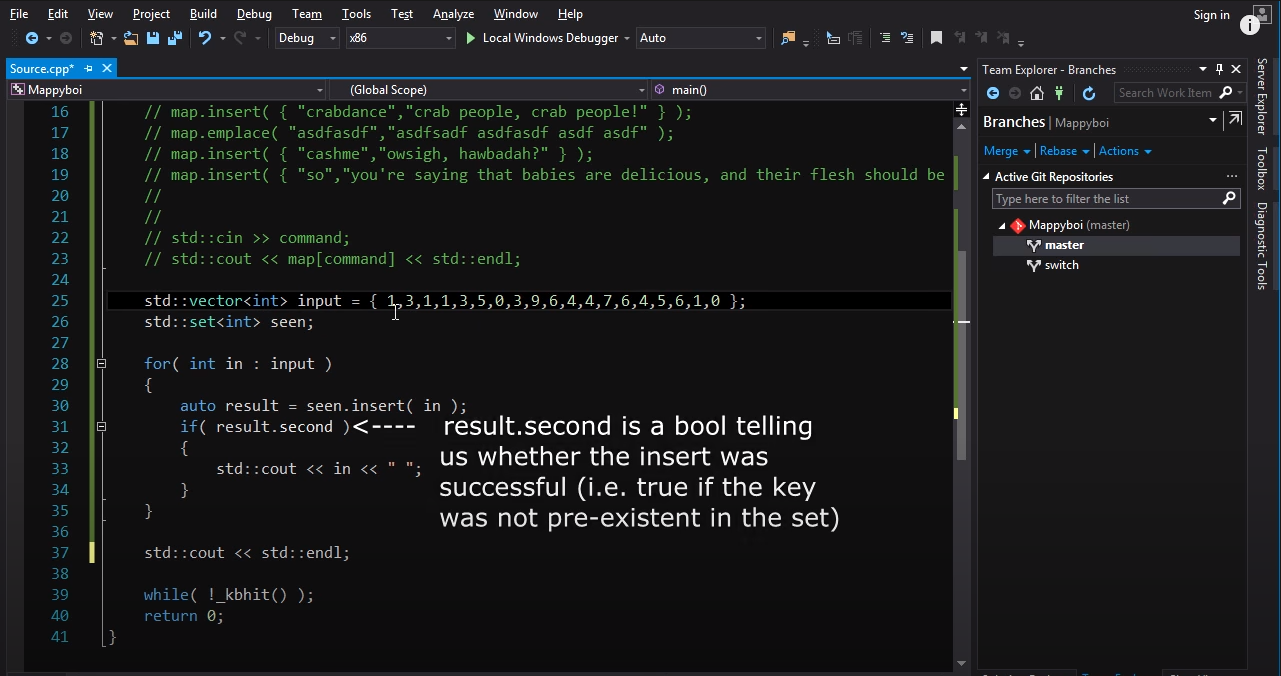
\includegraphics[width=1.2\textwidth, height=1.2\textheight, keepaspectratio]{./imgs/set_insert_second_operations.png}
	\caption{set}
	\label{fig:set_insert_second_operations}
\end{figure}

\subsubsection{multiset}

\textsf{\small \textbf{Definizione: } I \textbf{multiset} sono dei container associativi simili ai \textbf{set}, ma con un eccezione che molteplici elementi possono avere gli stessi valori.} \\

\begin{lstlisting}
	#include <iostream>
	#include <set>
	
	int main()
	{
		std::multiset<int> multiSet;
		
		multiSet.insert(9);
		multiSet.insert(9);
		multiSet.insert(9);
		
		std::cout << multiSet.count(9) << std::endl; //Output: 3
		
		multiSet.erase(multiSet.find(9)); // Rimuoverà solo uno dei tre 9.
		
		std::cout << multiSet.count(9) << std::endl; //Output: 2
		
		multiSet.erase(9); // Rimuoverà tutte le occorrenze del valore 9.
		
		std::cout << multiSet.count(9) << std::endl; //Output: 0
		
		return 0;
	}
\end{lstlisting}

\subsection{Pair}

\textsf{\small \textbf{Definizione: } Il \textbf{pair} (paio, coppia) serve per combinare due valori anche di tipi diversi. È praticamente usato per memorizzare delle \textbf{tuple} (sequenza di n elementi).} \break

\textsf{\small I \textbf{pair} sono contenuti nell'header \textbf{<utility>}.} \\

\textsf{\small Alcune proprietà del \textbf{pair}: } \\

\begin{itemize}
	\item \textsf{\small Il primo elemento viene referenziato come \emph{first} ed il secondo come \emph{second}.}
	\item \textsf{\small I \textbf{pair} possono essere assegnati, copiati, paragonati. Gli elementi in una mappa o hash\_map sono di tipo \textbf{pair} per default, dove \emph{first} è la chiave associata con il suo valore da \emph{second}.}
	\item \textsf{\small Per accedere agli elementi, usiamo il nome della variabile seguita dall'operatore \textbf{.} (punto) seguito dalla keyword \emph{first} o \emph{second}.}
\end{itemize}

\begin{lstlisting}
	#include <iostream>
	#include <utility> // Per i pair
	
	int main()
	{
		std::pair<char, int> pair;
		pair.first = 'L';
		pair.second = 1;
		
		std::cout << pair.first << " " << pair.second << std::endl; //Output: L 1
		
		std::pair<std::string, double> pair2("Ciao a tutti", 2.22);
		
		std::cout << pair2.first << " " << pair2.second << std::endl; //Output: Ciao a tutti 2.22
		
		std::pair<int, int> coords = {3, 2}; // Un'altra sintassi valida per dichiarare un pair.
		
		std::cout << coords.first << " " << coords.second << std::endl; //Output: 3 2
		
		return 0;
	}
\end{lstlisting}

\textsf{\small Alcune funzioni membro di \textbf{pair}: } \\

\begin{itemize}
	\item \textsf{\small \textbf{make\_pair()} : permette di creare un \textbf{pair} anche senza passare i parametri esplicitamente.}
	\item \textsf{\small \textbf{swap()} : scambia i contenuti di un pair con un altro.}
	\item \textsf{\small \textbf{tie()} : crea una tupla di referenze lvalues come argomento, per disimballare, spacchettare il pair in variabili separate. Ci sono anche alcune varianti al tie, con o senza \emph{ignore} che permette di ignorare un dato elemento dall'essere spacchettato.}
\end{itemize}

\begin{lstlisting}
	#include <iostream>
	#include <utility>
	
	int main()
	{
		// Esempio make\_pair
		std::pair<int, int> pair = std::make_pair(8, 2);
		std::cout << pair.first << " " << pair.second << std::endl; //Output: 8 2
		
		// Esempio swap
		std::pair<char, int> pair1 = std::make_pair('A', 0);
		std::pair<char, int> pair2 = std::make_pair('B', 1);
		
		std::cout << "Prima dello swap: " << pair1.first << " " << pair1.second << std::endl; //Output: Prima dello swap: A 0
		
		pair1.swap(pair2);
		
		std::cout << "Dopo lo swap: " << pair1.first << " " << pair1.second << std::endl; //Output: Dopo lo swap: B 1
		
		// Esempio tie
		std::pair<int, int> p1 = { 1, 2 };
		int a, b;
		std::tie(a, b) = p1;
		std::cout << a << " " << b << "\n"; // Output: 1 2
		
		std::pair<int, int> p2 = { 3, 4 };
		std::tie(a, ignore) = p2;
		
		std::cout << a << " " << b << "\n"; // Output: 3 2 (b è rimasto al valore precedente perché abbiamo messo ignore)
		return 0;
	}
\end{lstlisting}

\textsf{\small Possiamo usare gli operatori anche con i \textbf{pair}: } \\

\begin{enumerate}
	\item \textsf{\small \textbf{=} : implementato in questo modo: std::pair\& operator=(const std::pair\& pr).}
	\item \textsf{\small \textbf{==} per comparare due pair.}
	\item \textsf{\small \textbf{!=} per controllare se non sono uguali.}
	\item \textsf{\small \textbf{>=}, \textbf{<=} per controllare se è maggiore uguale o minore uguale.}
\end{enumerate}

\subsection{Tuple}

\textsf{\small \textbf{Definizione: } Una \textbf{tuple} (tupla) è un oggetto che può tenere un numero di elementi. Gli elementi possono essere di vari tipi.} \\

\textsf{\small Per poter usufruire delle tuple occorre importare \textbf{<tuple>}.} \break

\textsf{\small Varie operazioni che si possono fare sulle tuple: } \\

\begin{itemize}
	\item \textsf{\small \textbf{get()} : è usato per accedere ai valori della tupla e per poterli modificare. Accetta sia l'indice sia il nome come argomento per accedere ad un particolare elemento.}
	\item \textsf{\small \textbf{make\_tuple()} : usato per assegnare valori alla tupla.}
	\item \textsf{\small \textbf{tuple\_size} : restituisce il numero di elementi presenti nella tupla.}
	\item \textsf{\small \textbf{swap()} : scambia gli elementi di due tuple.}
	\item \textsf{\small \textbf{tie()} : spacchetta le tuple in variabili separate. Ci sono due varianti con e senza \textbf{ignore} per ignorare un particolare elemento della tupla e per non farlo spacchettare.}
	\item \textsf{\small \textbf{tuple\_cat()} : concatena due tuple e ne restituisce una nuova.}
\end{itemize}

\begin{lstlisting}
	#include <iostream>
	#include <tuple>
	
	int main()
	{
		std::tuple<char, int, float> tupla;
		tupla = std::make_tuple('S', 33, 52.6);
		
		std::cout << "Prima della modifica: " << std::get<0>(tupla) << " " << std::get<1>(tupla) << std::get<2>(tupla) << std::endl; //Output: Prima dela modifica: S 33 52.6
		
		// Usare get() per modificare i valori:
		std::get<0>(tupla) = 'T';
		std::get<2>(tupla) = 21.9;
		
		std::cout << "Dopo la modifica: " << std::get<0>(tupla) << " " << std::get<1>(tupla) << std::get<2>(tupla) << std::endl; //Output: Dopo la modifica: T 33 21.9
		
		// tuple\_size
		std::cout << "Il size della tupla è: " << std::tuple_size<decltype(tupla)>::value << std::endl; //Output: Il size della tupla è: 3
		
		// swap()
		
		std::tuple<char, int, float> tupla2('R', 54, 61.7);
		std::cout << "Elementi prima dello scambio: " << std::get<0>(tupla) << " " << std::get<1>(tupla) << " " << std::get<2>(tupla) << std::endl; //Output: Elementi prima dello scambio: T 33 21.9
		
		tupla.swap(tupla2);
		
		std::cout << "Elementi dopo lo scambio: " << std::get<0>(tupla) << " " << std::get<1>(tupla) << " " << std::get<2>(tupla) << std::endl; //Output: Elementi dopo lo scambio: R 54 61.7
		
		std::get<0>(tupla) = 'T';
		std::get<1>(tupla) = 33;
		std::get<2>(tupla) = 21.9;
		
		// tie()
		char c;
		int x;
		float f;
		
		std::tie(c, x, f) = tupla;
		
		std::cout << "I valori spacchettati della tupla sono: " << c << " " << x << " " << f << std::endl; //Output: I valori spacchettati della tupla sono: R 54 61.7
		
		// tuple\_cat()
		auto tupla3 = std::tuple_cat(tupla, tupla2);
		
		std::cout << "Gli elementi della nuova tupla sono: " << std::get<0>(tupla3) << " " << std::get<1>(tupla3) << " " << std::get<2>(tupla3) << " " << std::get<3>(tupla3) << " " << std::get<4>(tupla3) << " " << std::get<5>(tupla3) << " " << std::endl; //Output: Gli elementi della nuova tupla sono: T 33 21.9 R 54 61.7
		return 0;
	}
\end{lstlisting}

\subsection{Pair vs Tuple}

\textsf{\small Quali sono le differenze tra \textbf{pair} e \textbf{tuple}?} \\

\begin{tabular}{|c|c|}
	\hline
	\textbf{Pair} & \textbf{Tuple} \\
	\hline
	\textsf{\small Può contenere soltanto una coppia di valori.} & \textsf{\small Può contenere molteplici valori.} \\
	\hline
	\textsf{\small Un Pair è una specifico } & \textsf{\small È una classe template } \\
	\textsf{\small caso di tuple a due elementi.} & \textsf{\small con size fisso di valori eterogenei.} \\
	\hline
	\textsf{\small Non è difficile ottenere } & \textsf{\small È un po' più complicato } \\
	\textsf{\small i suoi elementi.} & \textsf{\small ottenere i suoi elementi.} \\
	\hline
	\textsf{\small Dovrebbe essere un po' più veloce di tuple.} & \textsf{\small È un po' più lenta se non ottimizzata.} \\
	\hline
\end{tabular}

\subsection{Hash Table}

\textsf{\small \textbf{Definizione: } L'\textbf{hashing} è una tecnica o processo di mappatura di chiavi e valori in una \textbf{hash table} attraverso una \textbf{hash function}.} \\

\textsf{\small Queste \textbf{hash function} potrebbero portare ad una collisione, ovvero quando due o più chiavi sono mappate allo stesso valore. Il \textbf{Chain Hashing} evita le collisioni: Ogni cella dell'\textbf{hash table} punta ad una \emph{lista linkata} di records che hanno lo stesso valore di \textbf{hash function}.} \\

%TODO: forse questo non è corretto?
\begin{figure}[H]
	\centering
	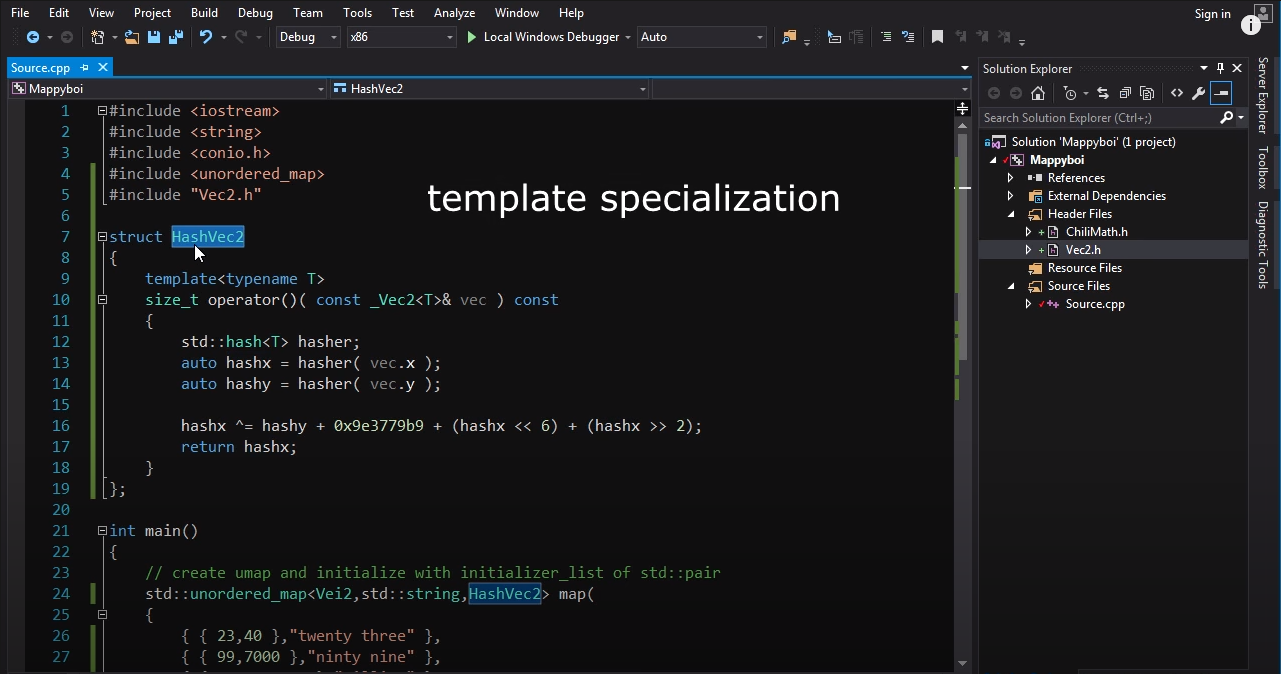
\includegraphics[width=1.2\textwidth, height=1.2\textheight, keepaspectratio]{./imgs/hash_table_template_specialization.png}
	\caption{Hash Table Template Specialization}
	\label{fig:hash_table_template_specialization}
\end{figure}

%TODO: sttrutture dati.

% -------------------------- SECTION: TYPE TRAITS ------------------------------------

\newpage

\section{Type Traits}

\textsf{\small \textbf{Definizione: } L'header \textbf{<type\_traits>} contiene un insieme di classi template per trasformare e controllare le proprietà dei tipi a compile-time.} \\

\textsf{\small Sono di solito usati per controllare gli errori dell'utente, sviluppo della programmazione generale e permettere ottimizzazioni.} \\

\textsf{\small La maggior parte dei \textbf{type traits} sono usati per controllare se un tipo soddisfa il criterio.} \\

\subsection{decltype}

\textsf{\small \textbf{Definizione: } \textbf{decltype} è un modo per specificare il  tipo: gli dai un'espressione e \textbf{decltype} ti restituisce il tipo (la tipologia della variabile) dell'espressione che gli hai passato.} \\

\textsf{\small Per esempio: se passi a \textbf{decltype(a)}, dove \emph{a} è il nome di una variabile (\emph{id-expression}) di tipo \textbf{int} allora \textbf{decltype} restituirà la tipologia di quella variabile che in questo caso è \textbf{int}. Se, invece, \emph{a} è un \textbf{lvalue} di tipo \emph{T} allora restituirà \emph{T \&} e se \emph{a} è un \textbf{rvalue} allora restituirà il tipo \emph{T}.} \\

\begin{lstlisting}
	int foo();
	int n = 9;
	
	// Usiamo decltype per ottenere la tipologia e la usiamo per assegnarla alle variabili.
	decltype(n) x = 18; // la variabile x è di tipo int. (id-expression)
	
	decltype((n)) y = x; // y è un int\& (n è un lvalue)
	
	decltype(foo()) z = foo(); // z è un int (rvalue)
	
	decltype(foo()) && w = foo(); // w è un int\&\&
	
	decltype((n)) && k = n; // k è int\& (\& \&\& collassa in \&)
\end{lstlisting}

\textsf{\small La forma speciale \textbf{decltype(auto)} deduce la tipologia della variabile dalla sua inizializzazione.} \\

\begin{lstlisting}
	const int a = 99;
	auto b = a;  // b ha tipo int
	decltype(auto) c = a; // c ha tipologia const int, ciò che è stato ritornato da decltype.
\end{lstlisting}

\textsf{\small Alcuni esempi su type\_traits: } \\

\begin{lstlisting}
	#include <iostream>
	#include <type_traits>
	
	// is\_function
	void f(){};
	int x(int a){return a};
	int(*y)(int)=x;
	
	// is\_class
	class MyClass{};
	
	int main()
	{
		// is\_function
		std::cout << std::boolalpha << "is_function<x>: " << std::is_function<decltype(x)>::value << " is_function<y>: " << std::is_function<decltype(y)>::value << std::endl; //Output: is\_function<x>: true is\_function<y>: false
		
		// is\_class
		std::cout << std::boolalpha << "is_class<MyClass>: " << std::is_class<MyClass>::value << std::endl; //Output: is\_class<MyClass>: true
		return 0;
	}
\end{lstlisting}

\begin{lstlisting}
	#include <iostream>
	#include <type_traits>
	
	template <typename T>
	void miServeUnPuntatore(T t) {
		std::static_assert(std::is_pointer<T>::value, "T deve essere di tipo puntatore");
	}
	
	//Overload per quando T non è un puntatore.
	template<typename T>
	typename std::enable_if<!std::is_pointer<T>::value>::type
	faccioQualcosaColPuntatore(T t) {
		//Corpo della funzione
	}
	
	//Overload per quando T è un puntatore
	template<typename T>
	typename std::enable_if<std::is_pointer<T>::value>::type 
	faccioQualcosaColPuntatore (T t) {
		//Corpo della funzione
	}
\end{lstlisting}

\textsf{\small Oltre a queste sono presenti tante altre funzioni.} \\

% ------------------ SECTION: RUN-TIME TYPE INFORMATION (RTTI) -----------------------

%TODO: spostare questa sezione dove ci sono i casts o lasciarla qui? Penso di lasciarla qui, credo.

\section{RTTI | Run-Time Type Information}

\textsf{\small \textbf{Definizione: } Il \textbf{Run-Time Type Information} (\emph{RTTI}) è un meccanismo che espone le informazioni del tipo di un oggetto a runtime ed è disponibile solo per le classi che hanno almeno una \textbf{funzione virtuale}. Permette di determinare la tipologia di un oggetto durante l'esecuzione del programma.} \\

\subsection{Runtime Casts}

\textsf{\small Il cast a runtime che controlla che il cast sia valido è l'approccio più semplice per verificare il tipo dell'oggetto a runtime usando un puntatore o una referenza. È utile quando abbiamo bisogno di fare un cast da un puntatore ad una classe base a una classe derivata.} \\

\textsf{\small Quando abbiamo a che fare con una gerarchia di classi, il casting degli oggetti è richiesto, di solito.} \\

\textsf{\small Ci sono due tipi di casting: } \\

\begin{itemize}
	\item \textsf{\small \textbf{Upcasting} : Quando un puntatore o referenza di una classe derivata è trattata come un puntatore a una classe base.}
	\item \textsf{\small \textbf{Downcasting} : Quando un puntatore o referenza a una classe base è convertito a puntatore di una classe derivata.}
\end{itemize}

\textsf{\small \textbf{dynamic\_cast} : in una gerarchia di ereditarietà è usato per il \emph{downcasting} di un puntatore di una classe base a una classe figlia.} \\

\textsf{\small Se riesce ritorna un puntatore al tipo convertito, altrimenti, fallisce se proviamo a fare un cast ad un tipo invalido come un puntatore che non è del tipo desiderato della classe derivata. Per esempio: \textbf{dynamic\_cast} non riesce a fare un cast ad un' altra classe se questa non ha almeno una funzione virtuale.} \\

\begin{lstlisting}
	#include <iostream>
	class B {
	};
	class D : public B {
	};
	
	int main()
	{
		B* b = new D;
		D* d = std::dynamic_cast<D*>(b); // Da errore perché B non ha nemmeno una funzione virtuale.
		return 0;
	}
	
\end{lstlisting}

% -------------------------- SECTION: TYPE INFO --------------------------------------

\section{Typeinfo}

\textsf{\small \textbf{Definizione: } Il file di intestazione \textbf{<typeinfo>} contiene implementazioni riguardo l'ottenere informazioni di un tipo, incluso il nome del tipo e modi per compararlo con altri tipi.} \\

\subsection{typeid}

\textsf{\small È usato quando servono le informazioni del tipo dinamico o a runtime di un oggetto.} \\
\textsf{\small È un'espressione lvalue.} \\

\begin{figure}[H]
	\centering
	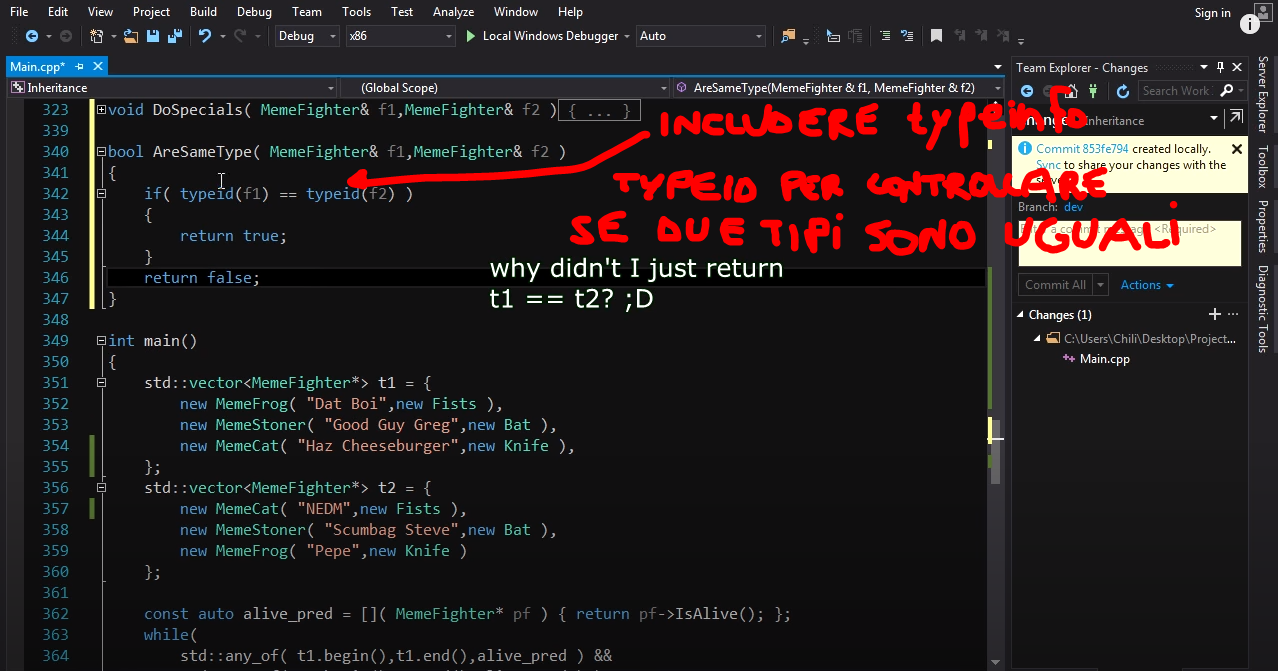
\includegraphics[width=1.2\textwidth, height=1.2\textheight, keepaspectratio]{./imgs/typeinfo_typeid.png}
	\caption{typeid}
	\label{fig:typeinfo_typeid}
\end{figure}

\begin{figure}[H]
	\centering
	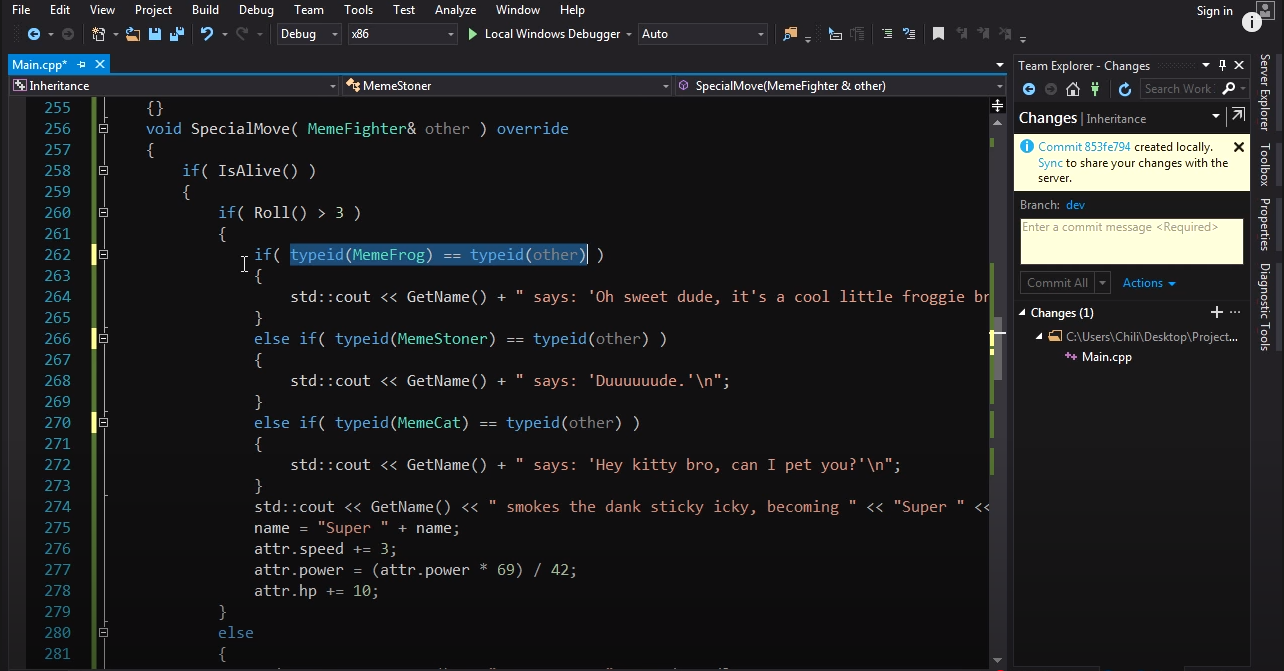
\includegraphics[width=1.2\textwidth, height=1.2\textheight, keepaspectratio]{./imgs/typeinfo_typeid_if.png}
	\caption{typeid}
	\label{fig:typeinfo_typeid_if}
\end{figure}

\textsf{\small In alcuni casi, \textbf{typeid} potrebbe essere più veloce di \textbf{dynamic cast}.} \\

\subsection{typeinfo}

\textsf{\small La funzione \textbf{typeinfo()} è un costrutto del compilatore GCC, non esiste (al momento) nel linguaggio e fa la stessa cosa di \textbf{decltype}, ovvero restituisce la tipologia di una variabile.} \\

% -------------------------- SECTION: ELLISSI ----------------------------------------

\newpage

\section{Ellissi}

\textsf{\small \textbf{Definizione: } Le \textbf{Ellissi}, ovvero i \textbf{...} (tre puntini) permettono ad una funzione di accettare un numero variabile di argomenti. È anche conosciuta come \emph{variable argument list}. } \\

\textsf{\small Di solito, le funzioni possono prendere solo un numero fisso di parametri, ma con le \textbf{ellissi} (\emph{ellipsis} in inglese) si possono passare tanti argomenti quanti se ne vuole. } \\

\textsf{\small Le \textbf{ellissi} sono definite nel file di intestazione \textbf{cstdarg}.} \\

\begin{lstlisting}
	#include <iostream>
	#include <cstdarg>
	
	double average(int count, ...)
	{
		// va\_list è usata per iterare sull'ellissi.
		va_list list;
		
		// Inizializza la posizione di va\_list.
		va_start(list, count);
		
		double average = 0.0;
		
		// Itera su ogni argomento passato.
		for(int i = 0; i < count; i++)
		{
			average += static_cast<double>(va_arg(list, int)) / count;
		}
	
		// Finisce l'utilizzo di va\_list.
		va_end(list);
		
		return average;
	}

	int main()
	{
		double avg = average(6, 3, 6, 9, 10, 7, 1);
		
		std::cout << "La media è: " << avg << std::endl; //Output: La media è: 6.0 ((3 + 6 + 9 + 10 + 7 + 1) / 6 = 36 / 6 = 6.0)
		return 0;
	}
\end{lstlisting}

\textsf{\small \textbf{Come funziona?}} \\

\begin{itemize}
	\item \textsf{\small \textbf{va\_list} : usato per accedere ai valori dell'ellissi.}
	\item \textsf{\small \textbf{va\_start} : punta alla \textbf{va\_list} all'inizio dell'ellissi.}
	\item \textsf{\small \textbf{va\_arg} : restituisce il valore a cui \textbf{va\_list} si sta riferendo e muove \textbf{va\_list} al prossimo parametro.}
	\item \textsf{\small \textbf{va\_end} : prende soltanto un argomento \textbf{va\_list} stessa. È usato per pulire la \textbf{va\_list}.}
\end{itemize}

\textsf{\small Non è molto usata in C++, perché al posto di usare l'\textbf{ellissi} possiamo passare come argomento un contenitore, come un \textbf{std::vector}, eccetera..} \\

% ------------------------ SECTION: INLINE FUNCTIONS ---------------------------------

\newpage

\section{Inline Functions}

\textsf{\small \textbf{Definizione: } Le \textbf{inline functions} (\emph{funzioni in linea}) sono un concetto molto potente. Se una funzione è \textbf{inline} il compilatore piazzerà una copia del codice di quella funzione ad ogni punto dove essa è chiamata.} \\

\textsf{\small Per le funzioni grandi, lunghe e/o che eseguono complesse tasks,	l'\emph{overhead} (sovrastante, sopra la testa, risorse in sovrappiù rispetto a quelle strettamente necessarie) è di solito insignificante comparato all'ammontare di tempo che la funzione ci mette per essere eseguita. Mentre, per quelle più piccole, le funzioni usate comunemente, il tempo necessario per fare la chiamata alla funzione è spesso molto di più rispetto a quello necessario per eseguirla.} \\

\textsf{\small Questo occorre per le piccole funzioni, perché il tempo di esecuzione è minore del tempo di cambio. (\emph{switching time}).} \break

\textsf{\small Quindi, la keyword \textbf{inline} nelle funzioni serve per ridurre l'\emph{overhead} nella chiamata alla funzione. È una funzione che viene espansa in linea quando viene chiamata. Quando la funzione \textbf{inline} viene chiamata, l'intero codice viene sostituito o inserito al momento della chiamata.} \\

\textsf{\small Il compilatore può ignorare il qualificato \textbf{inline} nel caso che la funzione definita \textbf{inline} sia più di una riga di codice.} \\

\textsf{\small È comune usarlo nelle funzioni delle classi. } \\

%TODO: è sbagliato questo esempio? Solo per le inline void?
\begin{lstlisting}
	#include <iostream>
	
	inline int max(int x, int y)
	{
		return x > y ? x : y;
	}

	int main()
	{
		std::cout << "max(3,9): " << max(3,9) << std::endl; //Output: 9
		std::cout << "max(21, 0): " << max(21, 0) << std::endl; //Output: 21
		std::cout << "max(4, 12): " << max(4, 12) << std::endl; //Output: 12
	}
\end{lstlisting}

\textsf{\small Inoltre il compilatore non la eseguirà \textbf{inline} se: } \\

\begin{itemize}
	\item \textsf{\small Se una funzione contiene un loop.}
	\item \textsf{\small Se una funzione contiene variabili statiche.}
	\item \textsf{\small Se una funzione è ricorsiva.}
	\item \textsf{\small Se il tipo di ritorno non è void e il return non esiste nel corpo della funzione.}
	\item \textsf{\small Se la funzione contiene switch o goto.}
\end{itemize}

\textsf{\small Le funzioni \textbf{inline} hanno i seguenti vantaggi: } \\

%TODO: "Questo non è possibile nelle funzioni normali" forse è da contestualizzare, argomentare, aggiungere spiegazioni e anche per la parte del flusso delle chiamate.

\begin{itemize}
	\item \textsf{\small Non occorre l'\emph{overhead} della funzione.}
	\item \textsf{\small Risparmia l'\emph{overhead} della push/pop di variabili nello stack quando è chiamata.}
	\item \textsf{\small Risparmia l'\emph{overhead} di una chiamata \textbf{return} da una funzione.}
	\item \textsf{\small Il compilatore potrebbe eseguire delle ottimizzazioni sul corpo della funzione. Questo non è possibile per le chiamate alle funzioni normali. Inoltre potrebbe ottimizzare anche il flusso delle chiamate.}  
	\item \textsf{\small Possono essere utili per gli \emph{embedded systems} perché possono produrre meno codice.}
\end{itemize}

\textsf{\small Gli svantaggi delle funzioni \textbf{inline}: } \\

\begin{itemize}
	\item \textsf{\small Le variabili aggiunte consumano più registri, il che potrebbe causare \emph{overhead} sul \emph{register variable resource utilization}.}
	\item \textsf{\small Se utilizzi troppe funzioni \textbf{inline} allora lo spazio del file binario eseguibile sarà molto grosso per via della duplicazione dello stesso codice.}
	\item \textsf{\small Troppe \textbf{inline} può anche ridurre le \emph{cache hit} (quando il contenuto che ti serve si trova nella cache e quindi viene caricato direttamente da lì al posto di richiederla dalla memoria primaria), riducendo la velocità di fetch dalla cache alla memoria primaria.}
	\item \textsf{\small Potrebbero aumentare l'\emph{overhead} del compilatore, perché se uno modifica una funzione \textbf{inline} allora il compilatore dovrebbe rimpiazzare tutto il codice un'altra volta, altrimenti continuerebbe ad essere eseguita con le vecchie funzionalità.}
	\item \textsf{\small Potrebbero non essere utili per gli \emph{embedded systems}, perché in essi lo spazio del codice è più importante della velocità.}
	\item \textsf{\small Potrebbero causare \emph{thrashing} (quando l'hard disk è in sovraccarico per via dello spostamento di informazioni tra memoria di sistema e memoria virtuale eccessivamente, portando a continui \emph{page faults}), perché l'\textbf{inline} potrebbe incrementare lo spazio del file eseguibile.}
\end{itemize}

\begin{lstlisting}
	#include <iostream>
	
	// Bad practice
	class A {
		public:
			inline int square(int s) // è ridondante
			{
				// Questa funzione è automaticamente inline.
			}
	};

	// Good practice
	clas A {
		public:
			int square(int s); // Dichiarazione prototipo della funzione
	};

	inline A::square(int s) // Definizione della funzione.
	{
		// Corpo della funzione.
	}
\end{lstlisting}

\textsf{\small Altre curiosità sulle funzioni \textbf{inline}: } \\

\textsf{\small È raccomandato di usare sempre le funzioni \textbf{inline} al posto delle macro. Le macros (in C++) non sono quasi mai necessarie e portano ad errori. Ci sono alcuni problemi con le macro: non possono accedere ai membri privati di una classe, sembrano delle funzioni, ma non lo sono, ed altro..} \\

\textsf{\small Tendenzialmente le funzioni che fanno I/O (input/output) non dovrebbero essere definite come \textbf{inline} perché spenderebbero un considerevole ammontare di tempo. Il tempo del codice di I/0 supera l'\emph{overhead} della chiamata alla funzione.} \break

\textsf{\small Un buon utilizzo delle funzioni \textbf{inline} possono essere di ottimo valore, ma un uso inappropriato non porterà a risultati migliori. Non porre tutte le funzioni \textbf{inline}. È meglio avere il minor numero di funzioni \textbf{inline} possibili.} \\

% ------------------------------------------------------------------------------------

%TODO: C++20 oppure in un capitolo a parte?

%TODO: Algorithm library: 

%TODO: C++20:
%TODO: ranges, concepts, constrained algorithms

%TODO: execution policies
%TODO: optionals
%TODO: heap, set, queue, priority_queue
%TODO: std::accumulate, std::any_of, find, search
%TODO: copy_if, copy_n_code
%TODO: std_count, count_if
%TODO: scan, equal code, fill_if, fill_n_code
%TODO: std_generate, inner product, iota, permutations
%TODO: sort
%TODO: lexicographic compare
%TODO: minmax, max, min
%TODO: mismatch
%TODO: std_transform
%TODO: std_unique_code
%TODO: SFINAE e concepts % oppure Le Classi, oppure boh.
	
	% ----------------------------- CONCETTI AVANZATI ------------------------------------

\chapter{Concetti Avanzati}

% Argomenti di questo capitolo:

% unique pointers
% smart pointers
% shared pointer
% weak pointers
% friend functions
% e make unique

%TODO: Copy-and-Swap Idiom?
%TODO: Signal Handling? (magari in un capitolo sul multithreading)
%TODO: Prevent Object Copy?
%TODO: Command Line Arguments?

%TODO: tecniche per debuggare codice?
%TODO: Writing C++ code efficiently in Competitive Programming?

%TODO: 7 Advance C++ Concepts: RAII, Return Type Resolver, Type Erasure, CRTP, Virtual Constructor, SFINAE, Proxy.

%TODO: pointer to function?

% std uniform real distribution

% C++ 20: Concepts, ranges, coroutines, template parameter list, modules, ecc.. (non qui, ma in Le gemme della libreria degli Algoritmi)

%TODO: Dependency Injection
%TODO: std::static_pointer_cast
%TODO: std::enable_share_from_this
%TODO: allocate_shared
%TODO: Allocator
%TODO: std::bad_alloc

%TODO: std::clamp (non è chi sa che cosa di avanzato, comunque).
%TODO: normal_distribution

% -------------------------- SECTION: INTRODUZIONE -----------------------------------

\section{Introduzione}

\textsf{\small In questo capitolo "finale" tratterò argomenti un po' più complessi o che almeno non mi verrebbe da mettere negli altri due capitoli precedenti.} \\

\textsf{\small Verranno trattati argomenti come gli smart pointers e quindi unique pointers, share pointers, weak pointers, le friend function, uniform real distribution e altri importanti concetti avanzati.} \\

% -------------------------- SECTION: FRIEND KEYWORD ---------------------------------

\newpage

\section{Friend Keyword}

\subsection{Friend Class}

\textsf{\small \textbf{Definizione: } La keyword \textbf{friend} è usata per accedere ai membri privati e protetti di una classe nella quale è dichiarata \textbf{friend}.} \\

\begin{lstlisting}
	#include <iostream>
	
	class A {
		public:
			A() { a = 0 };
			friend class B; // Classe amica.
			
		private:
			int a;
	};

	class B {
		public:
			void showA(A& x)
			{
				// Visto che B è un'amica di A, può accedere ai membri privati di A.
				std::cout << "A::a : " << x.a; 
			}
	};

	int main()
	{
		A a;
		B b;
		b.showA(); //Output: A::a : 0
		return 0;
	}
\end{lstlisting}

\subsection{Friend Function}

\textsf{\small \textbf{Definizione: } Come per le \textbf{classi friend}, una \textbf{funzione friend} ha accesso speciale ai membri privati e protetti.} \\

\textsf{\small Una \textbf{friend function} può essere: } \\

\begin{itemize}
	\item \textsf{\small Un membro di un'altra classe.}
	\item \textsf{\small Una funzione globale.}
\end{itemize}

\textsf{\small Alcuni importanti punti riguardo alle \textbf{friend} functions e classes: } \\

\begin{itemize}
	\item \textsf{\small Dovrebbero essere usate solo in maniera limitata. Troppe funzioni o classi \textbf{friend} diminuiscono l'encapsulazione.}
	\item \textsf{\small L'amicizia non è reciproca. Se la classe A è amica della classe B, allora B non è automaticamente amica di A.}
	\item \textsf{\small L'amicizia non è ereditata.}
	%\item \textsf{\small }
\end{itemize}

\begin{lstlisting}
	#include <iostream>
	
	class A {
		public:
			friend void printWidth( A a);
			void setWidth(double w);
			
		private:
			double width;
	};

	// Definizione della funzione membro di A.
	void A::setWidth(double w)
	{
		width = w;
	}

	// printWidth non è una funzione membra di nessuna classe.
	void printWidth( A a )
	{
		// Visto che la funzione printWidth è amica di A, può accedere direttamente a qualsiasi membro di A.
		std::cout << "Width di A: " << a.width << std::endl;
	}

	int main()
	{
		A a;
		
		a.setWidth(11.1);
		
		// Uso la funzione amica per stampare la width di a.
		printWidth( a ) ; //Output: Width di A: 11.1
		return 0;
	}
\end{lstlisting}

% -------------------------- SECTION: SMART POINTERS ---------------------------------

\newpage

\section{Smart Pointers}

\textsf{\small \textbf{Definizione: } } \\

%TODO: unique, share, weak, 
%TODO: std::make_unique vs std::unique_ptr
%TODO: std::make_shared

%TODO: problemi dei vecchi puntatori.

%TODO: std::static_pointer_cast
%TODO: std::enable_share_from_this
%TODO: allocate_shared
%TODO: Allocator
%TODO: std::bad_alloc

\subsection{unique pointers}

\textsf{\small \textbf{Definizione: } } \\

\subsection{share pointers}

\textsf{\small \textbf{Definizione: } } \\

\subsection{weak pointers}

\textsf{\small \textbf{Definizione: } } \\

% -------------------------- SECTION: UNIFORM REAL DISTRIBUTION ----------------------

\newpage

\section{Uniform Real Distribution}

\textsf{\small \textbf{Definizione: } } \\

%TODO: Dependency Injection

% -------------------------- SECTION: 7 CONCETTI AVANZATI ----------------------------

\newpage

%TODO: Questo come ultimo argomento del capitolo!

%TODO: Come prima cosa qui aggiungere quell'immagine sui 7 concetti avanzati.

%TODO: RAII, Return Type Resolver, Type Erasure, CRTP, Virtual Constructor, SFINAE, Proxy.

\section{7 Concetti Avanzati}

\subsection{RAII}

\textsf{\small \textbf{Definizione: } } \\ %TODO: scrivere che abbiamo già trattato questo argomento nel precedente capitolo oppure nel capitolo Concetti Intermedi, ma voglio comunque ripassarlo qui.

\subsection{Return Type Resolver}

\subsection{Type Erasure}

\subsection{CRTP}

\subsection{Virtual Constructor}

\subsection{SFINAE}

%TODO: tratterò questo argomento anche nel capitolo Le gemme della libreria degli Algoritmi.

\subsection{Proxy}

% ------------------------------------------------------------------------------------ % Concetti avanzati del linguaggio, C++20, concepts, ranges, ec..
	
\end{document}

% ----------------------------- END DOCUMENT -----------------------------------------